%   % !TEX root = ../../VIII,3_Rahmen-TeX_8-1.tex
%
%
%   Band VIII, 3 N.~??S01.08 ((\ref{dcc_06-2}))
%   Signatur/Tex-Datei: LH_35_09_23_015-020,37_04_059-060,37_05_091
%   RK-Nr. 41208 /8 + 57265 + 60235
%   Überschrift: De corporum concursus scheda secundo-sexta
%   Modul: Mechanik / Stoß ()
%   Datierung: Januar 1678
%   WZ: (Bl. 17; 19; 20; 60; 91) LEd-WZ 803017 = RK-WZ 1264 (insgesamt: fünf)
%   SZ: \pleibdashv \pleibvdash bzw. \leibdashv \leibvdash (insgesamt zwei in zweifacher Fassung)
%   Bilddateien (PDF): LH_35_09_23_015-020_d ((ex: lh0350923_017v-d2)) (insgesamt: eine)
%   Verzeichniseinträge: vollständig
%   \textls{} statt \textso{} (Ausnahme: Personenverzeichnis)
%
%
\selectlanguage{ngerman}%
\frenchspacing%
%
\begin{ledgroupsized}[r]{121mm}%
\footnotesize%
\pstart%
\noindent\textbf{Überlieferung:}
\pend%
\end{ledgroupsized}%
\begin{ledgroupsized}[r]{114mm}%
\footnotesize
\pstart%
\parindent -6,5mm%
\makebox[6,5mm][l]{\textit{L,\,A}}%
Konzept:
LH~XXXV~9,~23~Bl.~15\textendash20,
LH~XXXVII~4~Bl.~59\textendash60 und
LH~XXXVII~5~Bl.~91. 
Vier Bogen 2\textsuperscript{o}
(Bl.~15, 20; 16, 19; 17\textendash18; 59\textendash60)
und ein Blatt 2\textsuperscript{o}
(Bl.~91);
gleiches Wasserzeichen auf Bl.~17, 19, 20, 60 und 91;
Textverlust an den Rändern von Bl. 59
(der verlorene Text ist z.T. noch lesbar in dem 1967 aufgenommenen S-Film Nr.~116 der GWLB Hannover);
Papiererhaltungsmaßnahmen bei Bl.~59\textendash60 und 91.
%
Etwa zehneinhalb Seiten, % und zwei Zeilen,
die den Text von N.~\ref{dcc_06-1} %??S01\textsubscript{7} 
fortsetzen;
Bl.~%
15~r\textsuperscript{o}, % + 1 S.
15~v\textsuperscript{o}, % + 1 S.
17~v\textsuperscript{o}, % + 1 S.
18~r\textsuperscript{o}, % + 1 S.
18~v\textsuperscript{o}, % + 1 S.
19~r\textsuperscript{o}, % + 1 S.
59~r\textsuperscript{o}, % + 1 S.
59~v\textsuperscript{o} und % + 1 S.
91~r\textsuperscript{o} % + 1 S. = 9 S.
sind vollständig und zumeist ganzseitig beschrieben;
Bl.~%
16~v\textsuperscript{o}, % + 0,5 S.
20~r\textsuperscript{o} und % + 0,5 S. 
60~r\textsuperscript{o} % + 0,5 S. = 1,5 S.
halbseitig;
Bl.~%
17~r\textsuperscript{o}
um zwei Zeilen; % + 2 Z.
Bl.~%
16~r\textsuperscript{o}, % + 0 S.
19~v\textsuperscript{o}, % + 0 S.
20~v\textsuperscript{o} und % + 0 S.
60~v\textsuperscript{o} % + 0 S. = 10,5 S. + 2 Z.
sind leer;
Bl.~%
91~v\textsuperscript{o}
überliefert den Schlussteil von N.~\ref{dcc_10}. %??S01\textsubscript{12}.
% ((DCC Scheda decima = LH037_05_90-91))
%
Textfolge (nicht von Leibniz eindeutig festgelegt):
Bl.~%
15~r\textsuperscript{o},
15~v\textsuperscript{o},
20~r\textsuperscript{o},
% 16~v\textsuperscript{o},
59~r\textsuperscript{o},
59~v\textsuperscript{o},
60~r\textsuperscript{o},
(59~r\textsuperscript{o}),
(60~r\textsuperscript{o}),
% 16~v\textsuperscript{o},
% 17~r\textsuperscript{o},
91~r\textsuperscript{o},
17~r\textsuperscript{o},
17~v\textsuperscript{o},
18~r\textsuperscript{o},
(17~v\textsuperscript{o}),
(18~r\textsuperscript{o}),
18~v\textsuperscript{o}, % und
19~r\textsuperscript{o} und
16~v\textsuperscript{o}.
Die Tabellen auf Bl.~%
19~r\textsuperscript{o} (S.~\pageref{LH_35_09_23_019r_tab3}) und
Bl.~59~r\textsuperscript{o} bis
60~r\textsuperscript{o} (S.~\pageref{LH_37_04_059r_tabelle1in16}\textendash\pageref{LH_37_04_060r_tabelle1in1})
sind z.T. von Schreiberhand
% (wohl J.\,D. Brandshagen)\protect\index{Namensregister}{\textso{Brandshagen} (Brondhaguen), Jobst Dietrich 1659\textendash nach 1716}
mit Ergänzungen und Änderungen von Leibnizens Hand (\textit{LiA});
die in den Tabellen wiedergegebenen experimentellen Werte stammen von
\protect\index{Namensregister}{\textso{Regnauld} (Regnaud; Regnaldus), Fran\c{c}ois de 1626\textendash1689}%
\textsc{F.~Regnauld},
\cite{02021}Brief an B.~de Monconys vom 21.~Dezember 1655,
in
\protect\index{Namensregister}{\textso{Monconys} (Monconisius), Balthasar de 1611\textendash1665}%
\textsc{B.~de Monconys,}
\cite{00118}\title{Journal des voyages},
Teil III: \glqq Lettres escrittes à Monsieur de Monconys\grqq\
(Lyon 1666, S.~52\textendash55, getrennte Paginierung).
%Einige Randbemerkungen zu N.~\ref{dcc_06-2} %??S01\textsubscript{8} 
%sind von Leibniz erst \textit{post reformationem} hinzugefügt worden (siehe die Vorbemerkung, S.~\refpassage{dcc_Vorbemerkung_reform-1}{dcc_Vorbemerkung_reform-2}).
Siehe zur Textgenese von N.~\ref{dcc_06-2} %??S01\textsubscript{8} 
die editorische Vorbemerkung, S.~\refpassage{dcc_intro_VI-II_fzr-1}{dcc_intro_VI-II_fzr-2}.
\pend%
\end{ledgroupsized}%
%
\begin{ledgroupsized}[r]{114mm}
\footnotesize 
\pstart%
\parindent -6,5mm
\makebox[6,5mm][l]{\textit{E}}%
\textsc{Fichant} 1994, S.~125\textendash144\cite{01056}
(mit kommentierter französischer Übersetzung, S.~257\textendash277).
\pend
\end{ledgroupsized}
%
\selectlanguage{latin}%
\frenchspacing%
%
%
\count\Bfootins=1000%
\count\Afootins=1200%
\count\Cfootins=1000
%
\vspace{8mm}%
\normalsize%
\pstart%
\noindent%
%
\lbrack15~r\textsuperscript{o}\rbrack%    %    %    %    Blatt 15r
\hspace{40mm}
Scheda secundo-sexta%
\protect\index{Sachverzeichnis}{scheda}%
\edlabel{LH_35_09_23_015r_anfang_fhg}%
\hspace{30mm}
Januar. 1678
\pend%
\vspace{0.5em}%

\pstart%
\noindent%
\edtext{Ex his}{%
\lemma{Ex his}\Cfootnote{%
Der Text knüpft unmittelbar an das Ende von N.~\ref{dcc_06-1}, %??S01\textsubscript{7},
S.~\refpassage{LH_35_09_23_014v_ende}{LH_35_09_23_014v_ende} an.}}
concluditur universaliter,
corpore aliquo in aliud incurrente,%
\protect\index{Sachverzeichnis}{corpus incurrens}
fieri ex consideratione percussionis%
\protect\index{Sachverzeichnis}{percussio}
celeritatem excipientis%
\protect\index{Sachverzeichnis}{celeritas corporis excipientis}%
\rule[-2,5mm]{0mm}{0mm}
\pend%
%
\pstart%
\noindent%
\centering%
\edlabel{LH_35_09_23_015r_Ergebnis_gje-1}%
$\frac{\begin{array}{lll} +5 \smallfrown a^2 & +1 \smallfrown b^2 & +2ab\\ 
 \leibvdash\, 2 & \leibdashv\, 1 & \leibdashv\, 1 \end{array}}
 {\begin{array}{lll} +2a^2 & +2b^2 & +4ab
\end{array}}\; e,$%
\edlabel{LH_35_09_23_015r_Ergebnis_gje-2}%
\pend%
%
\pstart%
\noindent%
ubi patet
\rule[-0mm]{0mm}{4mm}%
posito \textit{b} aequ. \textit{a}
fieri hanc celeritatem aequ. \textit{e}.
\pend%
%
\pstart%
Breviter ergo,
et ut tutiores simus,
repetendus est calculus:%
\protect\index{Sachverzeichnis}{calculus}
tantum pro \textit{y}
%
\edtext{adhibendo \textit{w},}{%
\lemma{adhibendo \textit{w}}\Cfootnote{%
Die Setzung bleibt im Folgenden unbeachtet.
Siehe \textsc{Fichant} 1994, S.~125.\cite{01056}%
}}
%
quia alioqui litera \textit{y} uti soleo
pro celeritate excipientis.%
\protect\index{Sachverzeichnis}{celeritas corporis excipientis}%
\protect\index{Sachverzeichnis}{corpus excipiens}
\pend%
\newpage%
%
\pstart%
Corpus \textit{a},%
\protect\index{Sachverzeichnis}{corpus incurrens}
ejus celeritas \textit{e}.%
\protect\index{Sachverzeichnis}{celeritas corporis incurrentis}
Corpus \textit{b},%
\protect\index{Sachverzeichnis}{corpus excipiens}%
\protect\index{Sachverzeichnis}{corpus quiescens}
ejus celeritas 0.%
\protect\index{Sachverzeichnis}{celeritas corporis excipientis}
%
\edtext{Vis $v^2$ erit aequ. \textit{ae}.}{%
\lemma{\textit{Am Rand:}}\Afootnote{%
$v^2$ aequ. \textit{ae}
\newline%
}}
%
Si corpus \textit{a} abripiat%
\protect\index{Sachverzeichnis}{corpus abripiens}
secum corpus \textit{b},%
\protect\index{Sachverzeichnis}{corpus abreptum}
fiet celeritas abreptionis%
\protect\index{Sachverzeichnis}{abreptio}%
\protect\index{Sachverzeichnis}{celeritas abreptionis}
\rule[-4mm]{0pt}{9,5mm}%
$\displaystyle\frac{a}{a+b}e$
quam
%
\edtext{vocabimus \textit{s},%
\edtext{}{%
\lemma{\textit{Am Rand:}}\Afootnote{%
\textit{s} aequ. $\displaystyle\frac{a}{a+b}e$
\newline%
}}
%
quia ita}{%
\lemma{vocabimus}\Bfootnote{%
\textit{(1)}~\textit{t}, quia ita
\textit{(2)}~\textit{s}, quia ita%
~\textit{L}}}
%
simul moventur corpora,%
\protect\index{Sachverzeichnis}{corpora simul moventia}
quod fit,
cum nulla percussio contingit,%
\protect\index{Sachverzeichnis}{percussio nulla}
seu cum corpora sunt mollia%
\protect\index{Sachverzeichnis}{corpus molle}
et elastro carentia.%
\protect\index{Sachverzeichnis}{corpus elastro carens}
Porro vis percussionis tanta est,%
\protect\index{Sachverzeichnis}{vis percussionis}
quanta est vis%
\protect\index{Sachverzeichnis}{vis incurrentis perdita}
quam perdit incurrens per motum,%
\protect\index{Sachverzeichnis}{corpus incurrens}
quae utique est illa
quam daret excipienti,%
\protect\index{Sachverzeichnis}{corpus excipiens}
si simul progrederentur,
quae erit \textit{bs}.%
%
%\edtext{}{%
%\lemma{erit}\Bfootnote{%
%\textit{(1)}~\textit{sb}
%\textit{(2)}~\textit{bs}.%
%~\textit{L}}}%
%
\edtext{}{%
\lemma{\textit{Am Rand:}}\Afootnote{%
$p^2$ aequ. \textit{bs}
\newline%
}}
%
Hanc vim%
\protect\index{Sachverzeichnis}{vis incurrentis perdita}
potius elastro corporum dabit,%
\protect\index{Sachverzeichnis}{elastrum corporum concurrentium}
quia facilius est elastrum superare eousque
donec tensio elastri%
\protect\index{Sachverzeichnis}{tensio elastri}
aequalis fiat isti vi,%
\protect\index{Sachverzeichnis}{vis incurrentis perdita}
quia tunc quod supra
%
\edtext{addi deberet}{%
\lemma{addi}\Bfootnote{%
\textit{(1)}~posse
\textit{(2)}~deberet%
~\textit{L}}}
%
elastro,%
\protect\index{Sachverzeichnis}{elastrum corporum concurrentium}
%
\edtext{id}{%
\lemma{id}\Bfootnote{%
\textit{erg.~L}}}
%
potius corpori datur,%
\protect\index{Sachverzeichnis}{corpus excipiens}
quod minus resistet%
\protect\index{Sachverzeichnis}{resistentia corporis excipientis}
quam elastrum jam ita%
\protect\index{Sachverzeichnis}{resistentia elastri}
%
\edtext{tensum.%
\protect\index{Sachverzeichnis}{elastrum tensum}
Interea}{%
\lemma{tensum.}\Bfootnote{%
\textit{(1)}~Si
\textit{(2)}~Interea%
~\textit{L}}}
%
autem
%
\edtext{\lbrack tam\rbrack}{%
\lemma{tum}\Bfootnote{%
\textit{L~ändert Hrsg.}}}
%
vis%
\protect\index{Sachverzeichnis}{vis corporis incurrentis}
datur elastro,%
\protect\index{Sachverzeichnis}{elastrum corporis excipientis}
nihilominus residua vi%
\protect\index{Sachverzeichnis}{vis incurrentis residua}%
\protect\index{Sachverzeichnis}{vis residua}
\rule[-2mm]{0pt}{0mm}%
corpora simul pergere conabuntur,
ea residua vis erat%
\protect\index{Sachverzeichnis}{vis incurrentis residua}%
\protect\index{Sachverzeichnis}{vis residua}
%
\edtext{\textit{as}.
Vocabimus vim percussionis $p^2,$%
\protect\index{Sachverzeichnis}{vis percussionis}
fiet $p^2$}{%
\lemma{\textit{as}.}\Bfootnote{%
\textit{(1)}~Erit ergo $p^2$
\textit{(2)}~Vocabimus vim % percussionis $p^2,$ 
\lbrack...\rbrack\ fiet $p^2.$%
~\textit{L}}}
%
aequ. \textit{bs} vel $p^2$ aequ.
\rule[-3mm]{0pt}{7mm}%
$\displaystyle\frac{ab}{a+b}e.$%
%
\edtext{}{%
\lemma{\textit{Am Rand:}}\Afootnote{%
$p^2$ aequ. $\displaystyle\frac{ab}{a+b}e$
\newline%
}}
Ubi notandum
%
\edtext{%
percussionem eodem modo componi
\protect\rule[-3mm]{0pt}{7mm}%
ex utroque corpore.%
\protect\index{Sachverzeichnis}{percussio composita}%
}{%
\lemma{\textit{Am Rand:}}\Afootnote{%
Conclusio%
\protect\index{Sachverzeichnis}{conclusio}
verior quam modus probandi,%
\protect\index{Sachverzeichnis}{modus probandi}
ob errorem%
\protect\index{Sachverzeichnis}{error circa quantitatem motus}
circa quantitatem motus.%
\protect\index{Sachverzeichnis}{quantitas motus}%
%\newline%
}}
%
Vis autem in corpore \makebox[1.0\textwidth][s]{residua%
\protect\index{Sachverzeichnis}{vis incurrentis residua}
ademta vi percussionis,%
\protect\index{Sachverzeichnis}{vis percussionis ademta}
seu \textit{as},
\rule[-3mm]{0pt}{7mm}%
si dividatur per summam corporum%
\protect\index{Sachverzeichnis}{summa corporum concurrentium}
habebitur}%
\pend
\newpage
\pstart
\noindent celeritas%
\protect\index{Sachverzeichnis}{celeritas post percussionem}
qua corpora post percussionem pergere conantur,
\edtext{%
nempe
\protect\rule[-3mm]{0pt}{0mm}%
$\displaystyle\frac{as}{a+b}$ aequ.~$\pi,$%
}{%
\lemma{\textit{Am Rand:}}\Afootnote{%
$\pi$ aequ. $\displaystyle\frac{as}{a+b}$
\quad
$\pi$ aequ. $\displaystyle\frac{a}{a+b}\protect\fbox{2}\, ,e$%
\newline%
}}
%
id est
explicando \textit{s}
erit ipsum
$\displaystyle\frac{a^2}{a^2+2ab+b^2}e$
%
\edtext{}{%
{\xxref{LH_35_09_23_015r1}{LH_35_09_23_015r2}}%
{\lemma{aequ. $\pi.$}\Bfootnote{%
\textit{(1)}~Hinc \textlangle in\textrangle\ corpore incurren
\textit{(2)}~Porro percussio corpora%
~\textit{L}}}}%
%
\edlabel{LH_35_09_23_015r1}%
aequ. $\pi.$%
\protect\rule[-5mm]{0pt}{0mm}%
%
\edtext{}{%
\lemma{\textit{Am Ende des Absatzes:}}\Afootnote{Error puto.\newline%
}}
%
\pend%
%
\pstart%
Porro percussio corpora%
\edlabel{LH_35_09_23_015r2}
%
disjicere ac separare conatur,%
\protect\index{Sachverzeichnis}{percussio disjiciens}%
\protect\index{Sachverzeichnis}{percussio separans}
\rule[-3mm]{0pt}{5mm}%
vimque inter ipsa suam dividit.%
\protect\index{Sachverzeichnis}{vis percussionis divisa}
Ideo corpus incurrens \textit{a}%
\protect\index{Sachverzeichnis}{corpus incurrens}
duos habebit conatus,%
\protect\index{Sachverzeichnis}{conatus duplex}
unum pergendi celeritate $\pi,$%
\protect\index{Sachverzeichnis}{conatus pergendi}
alterum regrediendi vi%
\protect\index{Sachverzeichnis}{conatus regrediendi}%
\protect\index{Sachverzeichnis}{vis corporis incurrentis}
\rule[-3mm]{0pt}{7mm}%
$\displaystyle\frac{p^2}{2},$
id
%
\edtext{est celeritate%
\protect\index{Sachverzeichnis}{celeritas corporis incurrentis}%
}{%
\lemma{est}\Bfootnote{%
\textit{(1)}~vi
\textit{(2)}~celeritate%
~\textit{L}}}
%
\rule[-3mm]{0pt}{7mm}%
%
$\displaystyle\frac{p^2}{2a},$
quam vocemus \textit{r}.%
%
\edtext{}{%
\lemma{\textit{Am Rand:}}\Afootnote{%
\textit{r} aequ.
$\displaystyle\frac{p^2}{2a}$
aequ.
$\displaystyle\frac{b}{2a}s$ aequ.
$\displaystyle\frac{b}{2,\, a+b}e$
\newline%
}}
%
Et proinde movebitur eorum differentia,%
\protect\index{Sachverzeichnis}{differentia conatuum}
quae erit
$\pleibdashv\,\pi\;\pleibvdash\,r$
aequ.~$\epsilon.$%
%
\edtext{}{%
\lemma{\textit{Am Rand:}}\Afootnote{%
$\epsilon$ aequ. $\pleibdashv\,\pi\; \pleibvdash\,r,$
perget autem corpus \textit{a}%
\protect\index{Sachverzeichnis}{corpus pergens}
si $\pi$ major,
repelletur%
\protect\index{Sachverzeichnis}{corpus repulsum}
si \textit{r} major
ex his duabus.}}
%
Ex his autem minor quantitas,
id est $\pi$ vel \textit{r},
prout alterutra major fuerit,
%
\edtext{destruetur.%
\protect\index{Sachverzeichnis}{vis incurrentis destructa}
Minor quantitas,
ut generaliter exprimamus,
est
$\displaystyle\frac{\leibvdash\,\pi\; \leibdashv\,r + \pi + r}{2},$
id est}{%
\lemma{destruetur.}\Bfootnote{%
\textit{(1)}~Quod
\textit{(2)}~Id est % generaliter exprimamus 
\textit{(3)}~Minor quantitas ut generaliter exprimamus 
\textit{(a)}~destruetur: $\displaystyle\frac{\leibdashv\,\pi\; \leibvdash\,r + \pi\; \leibdashv\,r}{2},$ quae
\textit{(b)}~est $\displaystyle\frac{\leibvdash\,\pi\; \leibdashv\,r + \pi +r}{2},$ id est%
~\textit{L}}}
%
\rule[-3mm]{0pt}{7mm}%
differentia summae et differentiae dimidiata,
quae est quantitas minor.
\edlabel{LH_35_09_23_015r_notabiletheorema-1}%
(\protect\vphantom)%
Nam
%
\edtext{summa summae et differentiae dimidiata}{%
\lemma{summa}\Bfootnote{%
\textit{(1)}~earum
\textit{(2)}~summae et differentiae dimidiata%
~\textit{L}}}
%
est quantitas major.%
\protect\vphantom()%
\edlabel{LH_35_09_23_015r_notabiletheorema-2}
Destruetur ergo quantitas illa minor duplicata,%
\protect\index{Sachverzeichnis}{vis incurrentis destructa}
nempe:
$\pleibvdash\,\pi\; \pleibdashv\,r+\pi +r,$
id est vis
$\overline{\leibvdash\,\pi\,\leibdashv\, r+\pi +r}\; a,$
quae proinde transferenda est in corpus excipiens \textit{b},%
\protect\index{Sachverzeichnis}{vis incurrentis translata}
id est divisa per \textit{b}
dabit ipsi conatum%
\protect\index{Sachverzeichnis}{conatus corporis excipientis}
qui fiat celeritate%
\protect\index{Sachverzeichnis}{celeritas corporis excipientis}
\rule[-3mm]{0pt}{7mm}%
$\displaystyle\frac{a}{b}, \overline{\leibvdash\,\pi\; \leibdashv\,r+\pi +r}.$
%
Porro idem corpus \textit{b} excipiens%
\protect\index{Sachverzeichnis}{corpus excipiens}
jam habet celeritatem pergendi cum toto,%
\protect\index{Sachverzeichnis}{celeritas corporis excipientis}
nempe $\pi,$
item dimidiam vim percussionis,%
\protect\index{Sachverzeichnis}{vis percussionis dimidia}
seu conatum pergendi%
\protect\index{Sachverzeichnis}{conatus pergendi}
di-%
\makebox[1.0\textwidth][s]{midia vi percussionis%
\protect\index{Sachverzeichnis}{vis percussionis dimidia}
per ipsius magnitudinem divisa,%
\protect\index{Sachverzeichnis}{magnitudo corporis excipientis}
% \rule[-3mm]{0pt}{0mm}%
\edtext{$\displaystyle\frac{p^2}{2b},$
seu $\displaystyle\frac{s}{2},$
seu $\displaystyle\frac{a}{b}r.$}{%
\lemma{$\displaystyle\frac{p^2}{2b},$}\Bfootnote{%
\textit{(1)}~seu $\displaystyle\frac{s}{2}$
\textit{(2)}~seu $\displaystyle\frac{s}{2},$ seu $\displaystyle\frac{a}{b}r.$%
~\textit{L}}}
%
Habemus ergo}
\pend
\newpage
\pstart
\noindent summam celeritatis%
\protect\index{Sachverzeichnis}{summa celeritatum}
%
\edtext{qua progredietur}{%
\lemma{qua}\Bfootnote{%
\textit{(1)}~conatur
\textit{(2)}~progredietur%
~\textit{L}}}
%
excipiens%
\protect\index{Sachverzeichnis}{corpus excipiens}
\rule[-3mm]{0pt}{0mm}%
$\displaystyle\frac{a}{b},\,\overline{\leibvdash\,\pi\; \leibdashv\,r + \pi + r},\!, +\,\pi + \underset{\displaystyle\text{seu} +\frac{a}{b}r}{\displaystyle\frac{a}{2,\, a+b}e,}$
% \rule[-3mm]{0pt}{0mm}%
ergo
%
\edtext{fiet celeritas}{%
\lemma{fiet}\Bfootnote{%
\textit{(1)}~vis
\textit{(2)}~celeritas%
~\textit{L}}}
%
excipientis%
\protect\index{Sachverzeichnis}{celeritas corporis excipientis}
\rule[-3mm]{0pt}{7mm}%
$\displaystyle\frac{a}{b}\,\overline{\leibvdash\,\pi\; \leibdashv\,r+\pi +2r}+\pi$
\rule[-3mm]{0pt}{7mm}%
et celeritas incurrentis $\epsilon$ aequ. $\pleibdashv\,\pi\; \pleibvdash\,r.$
Id
%
\edtext{est si $\pi$ majus quam \textit{r},
tunc corpus}{%
\lemma{est}\Bfootnote{%
\textit{(1)}~corpus
\textit{(2)}~si $\pi$ % majus quam \textit{r}, 
\lbrack...\rbrack\ tunc corpus%
~\textit{L}}}
%
\textit{a} perget
\rule[-3mm]{0pt}{7mm}%
celeritate $+\,\pi -r,$
et corpus \textit{b} perget celeritate
\rule[-3mm]{0pt}{7mm}%
$\displaystyle\frac{3ar}{b}+\pi.$
\rule[-3mm]{0pt}{7mm}%
Si vero \textit{r} majus quam $\pi,$
tunc corpus \textit{a} repelletur%
\protect\index{Sachverzeichnis}{corpus repulsum}%
\protect\index{Sachverzeichnis}{corpus incurrens}
celeritate $r-\pi,$%
\protect\index{Sachverzeichnis}{celeritas repulsae}
at
%
\edtext{corpus \textit{b} perget}{%
\lemma{corpus \textit{b}}\Bfootnote{%
\textit{(1)}~repelletur
\textit{(2)}~perget%
~\textit{L}}}
%
celeritate%
\protect\index{Sachverzeichnis}{celeritas corporis excipientis}
\rule[-3mm]{0pt}{7mm}%
$\displaystyle\frac{a}{b}\,\overline{2\pi +r},\, +\pi.$
%
\lbrack15~v\textsuperscript{o}\rbrack%    %    %    %    Blatt 15v
%
\pend%
%
\pstart%
Ut vero literas $\pi,$ \textit{r} explicemus,%
\protect\index{Sachverzeichnis}{litera}
retenta signorum ambiguitate,%
\protect\index{Sachverzeichnis}{ambiguitas signorum}
substituemus pro $\pi,$
\rule[-3mm]{0pt}{7mm}%
$\displaystyle\frac{a^2}{a^2 + b^2 + 2ab}e,$
et pro \textit{r}
ponemus
\rule[-3mm]{0pt}{7mm}%
$\displaystyle\frac{b}{2a+2b}e.$
%\pend%
%%
%\pstart%
Itaque pro $\pleibdashv\,\pi\; \pleibvdash\,r$
fiet:
\newline%
\rule[-4mm]{0pt}{10,5mm}%
$\displaystyle\frac{\leibdashv\,2a^2\, \leibvdash\,ab \;\leibvdash\,b^2}{2a^2 + 4ab + 2b^2}e$
aequ. $\epsilon,$
%\newline%
et pro
\rule[-4mm]{0pt}{10mm}%
$\displaystyle\frac{a}{b}\,\overline{%
\leibvdash\,\pi\; \leibdashv\,r + \pi + 2r} + \pi$
fiet
\newline%
\rule[-4mm]{0pt}{10mm}%
$\displaystyle\frac{%
\begin{array}{lll}\leibvdash\,1 \smallfrown 2a^3 & \leibdashv\,1 \smallfrown a^2b & +\,2a^2b\\ +\,1 & +\,2 \; \ ab^2 &\end{array}%
}{+\,2a^2b +4ab^2 +2b^3}\,e,$
% \newline%
%
\edtext{vel}{%
\lemma{vel}\Cfootnote{%
Im linken Ausdruck fehlen im Nenner eigentlich die Summanden $\, \pleibdashv ab^2$ und $+\, 2a^2b.$
Der rechte Ausdruck ist hingegen richtig.}}
%
$\displaystyle\frac{%
\begin{array}{lll}\leibvdash\,1 \smallfrown 2a^3 & \leibdashv\,1\smallfrown a^2b & \leibdashv\,1 \smallfrown ab^2\\ +\,1 & +\,4 & +\,2 \end{array}%
}{+\,2a^2b + 4ab^2 + 2b^3}\,e.$%
\rule[-2mm]{0pt}{10mm}
%
\pend%
%
\pstart%
Porro in valore ipsius $\epsilon$ invento patet,%
\protect\index{Sachverzeichnis}{valor inventus}
\rule[-0mm]{0pt}{5mm}%
%
\newline%
\edtext{si corpus \textit{a} sit majus}{%
\lemma{si}\Bfootnote{%
\textit{(1)}~\textit{a} sit
\textit{(2)}~corpus \textit{a} sit majus%
~\textit{L}}}
%
corpore \textit{b},
etiam
%
\edtext{quantitatem}{%
\lemma{quantitatem}\Bfootnote{%
\textit{erg.~L}}}
%
$2a^2$ esse majorem quantitate
%
\edtext{}{%
{\xxref{LH_35_09_23_015v1}{LH_35_09_23_015v2}}%
{\lemma{$ab+b^2$}\Bfootnote{%
\textit{(1)}~nam $a^2+$
\textit{(2)}~et contra % si \textit{b} sit majus quam \textit{a}, esse 
\lbrack...\rbrack\ minorem nam
\textbar~si \textit{a} % \protect\begin{tabular}[t]{c} majus\\ minus \protect\end{tabular} quam 
\lbrack...\rbrack\ \textit{b} erit \textit{erg.}~%
\textbar\ $a^2+a^2$%
~\textit{L}}}}%
%
\edlabel{LH_35_09_23_015v1}%
$ab+b^2,$
\newline%
et contra
si \textit{b} sit majus quam \textit{a},
esse minorem,
\newline%
nam si \textit{a}%
\hspace{-0,75mm}%
\begin{tabular}[t]{l}%
majus\\ minus%
\end{tabular}%
\hspace{-0,75mm}%
quam \textit{b},
erit $a^2+ a^2$%
\edlabel{LH_35_09_23_015v2}%
%
\hspace{-0,75mm}%
\begin{tabular}[t]{l}%
majus\\ minus%
\end{tabular}%
\hspace{-0,75mm}%
%\advanceline{1}
quam $ab+b^2,$
\newline%
quia $a^2$%
\hspace{-0,75mm}%
\begin{tabular}[t]{l}%
majus\\ minus%
\end{tabular}%
\hspace{-0,75mm}%
quam $b^2,$
et $a^2$%
\hspace{-0,75mm}%
\begin{tabular}[t]{l}%
majus\\ minus%
\end{tabular}%
\hspace{-0,75mm}%
quam \textit{ab}.
\pend%
%
\pstart%
Quod si \textit{a}, \textit{b} corpora sint aequalia,%
\protect\index{Sachverzeichnis}{corpora aequalia}
erunt et hae duae quantitates aequales,
fietque $\epsilon$ aequ. 0,
%
\edtext{quod aliunde notum
%
%\edtext{}{%
%{\xxref{LH_35_09_23_015v5}{LH_35_09_23_015v6}}%
%{\lemma{est.}\Bfootnote{%
%\textit{(1)}~Hinc patet si corpus \textit{a} sit \protect\begin{tabular}[t]{c} majus\\ minus \protect\end{tabular} corpore \textit{b} tunc $\pleibdashv$ significare
%\textit{(2)}~Hinc si % corpus \textit{a} \protect\begin{tabular}[t]{c} majus\\ minus \protect\end{tabular} corpore \textit{b} fiet $\leibdashv$ aequ. \protect\begin{tabular}[t]{c} $+$ \\ $-$ \protect\end{tabular} $\leibvdash$ 
%\lbrack...\rbrack\ aequ. \protect\begin{tabular}[t]{c} $-$ \\ $+$ \protect\end{tabular}.%
%~\textit{L}}}}%
%
\edlabel{LH_35_09_23_015v5}%
est.}{%
\lemma{quod \lbrack...\rbrack\ est}\Cfootnote{%
Vgl. N.~\ref{dcc_01}, %??S01\textsubscript{1}, 
S.~\refpassage{LH_35_09_23_001r_incurr-in-aequ-quiesc-1}{LH_35_09_23_001r_incurr-in-aequ-quiesc-2}.%
}}
%
\pend%
\newpage%
%
\pstart%
%
%%%%%%%%%%%%%%%%    Nebenrechnungen: Anfang
%
\edtext{}{%
{\xxref{LH_35_09_23_015v_nebenrechnungen-1}{LH_35_09_23_015v_nebenrechnungen-2}}%
{\lemma{\textit{Am Rand verstreut, wohl Hilfsrechnungen zu Bl.~91~r\textsuperscript{o}:}}%
\Afootnote{\newline%
\newline%
%
%
\protect\begin{array}[b]{r}
15,\smallfrown 15\phantom{5}\\
75\phantom{5}\\
15\phantom{55}\\
\overline{225}\phantom{5}\\
225\\
\overline{\phantom{2255}}
\protect\end{array}
%
\hspace*{15mm}
%
$\protect\begin{array}[b]{r}
16\\16\\ \overline{\phantom{2}96}\\16\phantom{6}\\ \overline{256}\\3\\\overline{768}\\-18\\\overline{750}
\protect\end{array}
%
\hspace*{10mm}
%
\protect\begin{array}[b]{r}
750\\ 375\\ \cancel{1}\stackrel{\displaystyle 8}{9}6\\ \cancel{3}\cancel{7}\cancel{5}\\ \cancel{2}\cancel{8}\cancel{9}
\protect\end{array}
%
\protect\begin{array}[b]{r}
17\\ 17\\ \overline{119}\\ 17\phantom{9}\\ \overline{289}\\ \\ f\;1\displaystyle\frac{86}{289}\\
\protect\end{array}
%
\hspace*{20mm}
%
\protect\begin{array}[b]{r}
578\\
16\\
\overline{3468}\\
578\phantom{8}\\
\overline{9248}
\protect\end{array}\\
%
\hspace*{68mm}\text{circiter}\;1\frac{1}{3}$%
}}}%
%
%%%%%%%%%%%%%%%%%%%    Nebenrechnungen: Ende
%
Hinc%
\edlabel{LH_35_09_23_015v_nebenrechnungen-1}
si corpus \textit{a}%
\hspace{-0,75mm}%
\begin{tabular}[t]{l}%
majus\\ minus%
\end{tabular}%
\hspace{-0,75mm}%
corpore \textit{b},
fiet:
\quad
$\leibdashv\ $ aequ.%
\hspace{-0,75mm}%
\begin{tabular}[t]{l}%
$+$\\
$-$%
\end{tabular}%
\hspace{-0,75mm}%
\quad
$\leibvdash\ $ aequ.%
\hspace{-0,75mm}%
\begin{tabular}[t]{l}%
$-$\\
$+$%
\end{tabular}.%
\edlabel{LH_35_09_23_015v6}
%
\pend%
%
\pstart%
Ergo si corpus%
\hspace{-0,5mm}%
\begin{tabular}[t]{l}%
majus\\ minus\\ aequale%
% \reversemarginpar\marginnote{{\scriptsize 10}}
\end{tabular}%
\hspace{-2,5mm}%
incurrit in%
\hspace{-0,5mm}%
\begin{tabular}[t]{l}%
minus\\ majus\\ aequale%
\end{tabular}%
\hspace{-2,5mm}%
% \advanceline{2}
semper%
\hspace{-0,5mm}%
\begin{tabular}[t]{l}%
progreditur\\ repellitur\\ quiescit%
\end{tabular}%
\hspace{-1,5mm}%
%\advanceline{3}
post concursum.%
\protect\index{Sachverzeichnis}{corpus incurrens majus}%
\protect\index{Sachverzeichnis}{corpus excipiens majus}%
\protect\index{Sachverzeichnis}{corpus incurrens minus}%
\protect\index{Sachverzeichnis}{corpus excipiens minus}%
\protect\index{Sachverzeichnis}{corpus majus in minus}%
\protect\index{Sachverzeichnis}{corpus minus in majus}%
\protect\index{Sachverzeichnis}{corpus progrediens}%
\protect\index{Sachverzeichnis}{corpus repulsum}%
\protect\index{Sachverzeichnis}{corpus quiescens}%
\protect\index{Sachverzeichnis}{concursus corporum}
\pend%
%
\pstart%
Hinc si corpus majus incurrit in minus fiet $\epsilon,$%
\rule[-2mm]{0pt}{6mm}
% \newline%
seu celeritas incurrentis%
\protect\index{Sachverzeichnis}{celeritas corporis incurrentis}
qua pergit
\rule[-3mm]{0pt}{3mm}%
\edlabel{LH_35_09_23_015v_Gleichung_1-1}%
$\displaystyle\frac{+2a^2-ab-b^2}{2,\, a^2+2ab+b^2}e,$%
\edlabel{LH_35_09_23_015v_Gleichung_1-2}
%
\edtext{\lbrack seu\rbrack}{%
\lemma{seu}\Bfootnote{%
\textit{erg. Hrsg. nach~E, S.~127}}}
%
\edtext{erit
$\displaystyle\frac{a}{a+b}\,\protect\fbox{2}\,,e,\!,\, -\,\displaystyle\frac{b}{2,\, a+b}e,$}{%
\lemma{erit}\Bfootnote{%
\hspace{-0,5mm}%
$\displaystyle\frac{a}{a+b}\,\protect\fbox{2}\,,e,\!,\, -\,\displaystyle\frac{b}{2,\, a+b}e,$
\textit{erg.~L}}}
%
% \newline%
\rule[-4mm]{0pt}{7,5mm}%
et celeritas impulsi%
\protect\index{Sachverzeichnis}{celeritas corporis impulsi}
seu excipientis%
\protect\index{Sachverzeichnis}{celeritas corporis excipientis}
\rule[-4mm]{0pt}{7,5mm}%
\edlabel{LH_35_09_23_015v_Gleichung_2-1}%
$\displaystyle\frac{5a^2 + 3ab}{2,\, a^2 + b^2 + 2ab} e$%
\edlabel{LH_35_09_23_015v_Gleichung_2-2}
% \hspace{-0,5mm}%
% $\protect\begin{array}[t]{l}$
seu
$\overline{\displaystyle\frac{3a}{2,\, a+b},\!, +\,\displaystyle\frac{a}{a+b}\,\protect\fbox{2}}\; e$ aequ.
%
\edtext{$\upsilon,$}{%
\lemma{$\upsilon$}\Cfootnote{%
In N.~\ref{dcc_06-2} %??S01\textsubscript{8}
wird statt \textit{y} das griechische Ypsilon verwendet.}}
%
seu
$\displaystyle\frac{3ra}{b} + \pi,$
est enim \textit{r} \mbox{aequ.}
\rule[-4mm]{0pt}{0mm}%
$\displaystyle\frac{b}{2,\, a+b}e,$
seu
$\displaystyle\frac{3p^2}{2b} + \pi,$
% \advanceline{2}
% \reversemarginpar\marginnote{{\scriptsize 15}}
% \newline%
\edtext{seu
\lbrack conatus\rbrack%
\protect\index{Sachverzeichnis}{conatus pergendi}%
\protect\index{Sachverzeichnis}{conatus communis}
%
pergendi
\lbrack communis\rbrack\
cum sesquialtera}{%
\lemma{seu}\Bfootnote{\hspace{-0,5mm}%
\textbar~conatum \textit{ändert Hrsg.}~%
\textbar\ pergendi
\textit{(1)}~corporis incurrentis
\textit{(2)}~\textbar~communem \textit{ändert Hrsg.}~\textbar\ 
\textit{(a)}~triplo
\textit{(b)}~cum sesquialtera%
~\textit{L}}}
%
vi percussionis.%
\protect\index{Sachverzeichnis}{vis percussionis}
\rule[-3mm]{0pt}{6mm}%
Quod etiam facile patet ex positis,
\rule[-3mm]{0pt}{6mm}%
quia tum dimidiam habet vim percussionis statim receptam,%
\protect\index{Sachverzeichnis}{vis percussionis dimidia}%
\protect\index{Sachverzeichnis}{vis percussionis recepta}
tum alteram dimidiam una cum alia 
\edlabel{LH_35_09_23_015v3}%
in incurrente%
\protect\index{Sachverzeichnis}{corpus incurrens}
%
\edtext{}{%
{\xxref{LH_35_09_23_015v3}{LH_35_09_23_015v4}}%
{\lemma{in}\Bfootnote{%
\textit{(1)}~excipiente de
\textit{(2)}~incurrente destructam.
\textit{(a)}~Si vero minus incurrit in majus
\textit{(b)}~Ubi illud % notandum, si ab $\upsilon$ 
\lbrack...\rbrack\ auferatur $\epsilon$%
~\textit{L}}}}%
%
\rule[-3mm]{0pt}{6mm}%
destructam.%
\protect\index{Sachverzeichnis}{vis incurrentis destructa}%
\protect\index{Sachverzeichnis}{vis destructa}
\pend%
\newpage%
%
\pstart%
Ubi illud notandum,
% \rule[-0mm]{0pt}{6mm}%
si ab $\upsilon$ auferatur $\epsilon$%
\edlabel{LH_35_09_23_015v4}
fieri
$\upsilon - \epsilon$
distantiam corporum post concursum%
\protect\index{Sachverzeichnis}{distantia corporum post concursum}
\rule[-3mm]{0pt}{7mm}%
%
$\displaystyle\frac{3a+b}{2,\,a+b}e$
sive
$e+\displaystyle\frac{a-b}{2,\,a+b}\edtext{[e].$}{%
\lemma{\textit{e}}\Bfootnote{%
\textit{erg. Hrsg. nach~E, s.~128}}}%
%
\rule[-3mm]{0pt}{7mm}
%
\edtext{%
Est ergo $\delta$
seu distantia corporum
major quam \textit{e}
distantia prior.%
\protect\index{Sachverzeichnis}{distantia corporum ante concursum}%
}{%
\lemma{\textit{Am Rand:}}\Afootnote{%
$\delta$ aequ. $e+\displaystyle\frac{a-b}{2,a+b}$}}
%
\pend%
%
\pstart%
Quaeramus et quanto sit $\upsilon$ major quam
%
\edtext{[\textit{e}],}{%
\lemma{$\upsilon$}\Bfootnote{%
\textit{L~ändert Hrsg. nach~E, S.~128}}}
%
seu quaeramus $\upsilon -e,$
fiet:\\
%\rule[-3mm]{0pt}{7mm}%
\rule[-4mm]{0pt}{10mm}%
$\displaystyle\frac{5a^2+3ab-2a^2-2b^2-4ab}{2,\, a^2+b^2+2ab}\, e$ aequ.
\rule[-3mm]{0pt}{7mm}%
$\displaystyle\frac{3a^2-ab-2b^2}{2,\, a^2+b^2+2ab}\, e,$
%\newline%
qui est excessus celeritatis excipientis%
\protect\index{Sachverzeichnis}{excessus celeritatis excipientis}
supra celeritatem incursus,%
\protect\index{Sachverzeichnis}{celeritas incursus}
nam $3a^2$ semper major quam $ab+2b^2,$
quamdiu \textit{a} major quam \textit{b},
ut patet.
Eritque tanto major,
quanto major est celeritas \textit{e},%
\protect\index{Sachverzeichnis}{celeritas incursus}
tantoque minor
quanto magis corpora accedunt%
\protect\index{Sachverzeichnis}{corpora concurrentia}%
\protect\index{Sachverzeichnis}{aequalitas corporum concurrentium}
%
\edlabel{LH_35_09_23_015v_dftks-1}%
ad \lbrack aequalitatem\rbrack.%
\edtext{}{%
{\xxref{LH_35_09_23_015v_dftks-1}{LH_35_09_23_020r_dftks-2}}%
{\lemma{ad}\Bfootnote{\hspace{-0,5mm}%
\textbar~celeritatem \textit{ändert Hrsg. nach~E, S.~128}~\textbar~%
\textit{(1)}~Sit \textit{e} si ad $\epsilon$ addatur $e+\displaystyle\frac{a^2-b^2}{2,\overline{a+b}^2}\,e,$ seu $\displaystyle\frac{a-b}{2,\, a+b}\, e$ fit $\upsilon,$ seu $\displaystyle\frac{2ae+2be+ae-be}{}$
\textit{(2)}~\lbrack20~r\textsuperscript{o}\rbrack\ Addantur in
\lbrack...\rbrack\ prodire \textit{ae}
~\textit{L}}}}%
\edlabel{LH_35_09_23_015v_nebenrechnungen-2}
%
\lbrack20~r\textsuperscript{o}\rbrack%    %    %    %    Blatt 20v
%
\pend%
%
\pstart%
Addantur in unum $a\epsilon$ et $b\upsilon,$%
\edlabel{LH_35_09_23_020r_dftks-2}
debet prodire \textit{ae},
quae est proba calculi:%
\protect\index{Sachverzeichnis}{proba calculi}%
\protect\index{Sachverzeichnis}{calculus}
\newline%
\rule[-4mm]{0pt}{12mm}%
$\displaystyle\frac{2a^3-a^2b-ab^2+5a^2b+3ab^2}{2a^2+4ab+2b^2}\,e,$
% \newline%
sive
$\displaystyle\frac{%
2a^2 \raisebox{-2.2mm}
{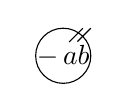
\begin{tikzpicture} \draw (0,0) circle (0.35cm) node at (0,0) {$-\,ab$}; \draw (.18,.18) -- (.35,.35); \draw (.075,.175) -- (.25,.35); \end{tikzpicture}}\;
\ovalbox{$-\,b^2$} + 
\overset{4}{\raisebox{-1.5mm}{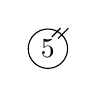
\begin{tikzpicture} \draw (0,0) circle (0.25cm) node at (0,0) {5}; \draw (.13,.13) -- (.26,.26); \draw (.05,.15) -- (.16,.26); \end{tikzpicture}}}\;ab + 
\overset{2}{\ovalbox{3}}\;b^2%
}{2a^2+4ab+2b^2}\,ae,$
\newline%
sive
\rule[-3mm]{0pt}{7mm}%
$\displaystyle\frac{2a^2+4ab+2b^2}{2a^2+4ab+2b^2}\,ae,$
sive \textit{ae}.
\pend%
%
\pstart%
Quando incurrens%
\protect\index{Sachverzeichnis}{corpus incurrens}
est minus excipiente%
\protect\index{Sachverzeichnis}{corpus excipiens}
\rule[-2mm]{0pt}{6mm}%
fiet:
\newline%
$\upsilon$ aequ.
\rule[-2mm]{0pt}{5mm}%
$\displaystyle\frac{4a^3 + 3a^2b + ab^2}{2a^2b + 4ab^2 + 2b^3}\,e$
et $\epsilon$ aequ.
\rule[-2mm]{0pt}{5mm}%
$\displaystyle\frac{+\,b^2 + ab - 2a^2}{2a^2 + 4ab + 2b^2}\,e.$
\pend%
%
\pstart%
Multiplicetur $\upsilon$ per \textit{b},
\rule[-0mm]{0pt}{5mm}%
et $\epsilon$ per \textit{a},
et producta addantur
fiet:
\newline%
$\displaystyle\frac{%
\overset{2}{\ovalbox{4}}%
\,a^3\;%
\overset{4}{\raisebox{-2.0mm}%
{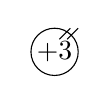
\begin{tikzpicture} \draw (0,0) circle (0.30cm) node {$+3$}; \draw (.16,.16) -- (.30,.30); \draw(.06,.16) -- (.20,.30); \end{tikzpicture}}%
}\,a^2b\
\overset{2}{\raisebox{-1,8mm}%
{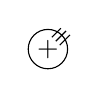
\begin{tikzpicture} \draw (0,0) circle (0.25cm) node {$+$}; \draw (.1,.1) -- (.23,.23); \draw (.05,.15) -- (.165,.265); \draw (.15,.05) -- (.28,.18); \end{tikzpicture}}%
}ab^2,\
\raisebox{-2,5mm}%
{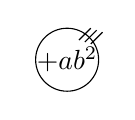
\begin{tikzpicture} \draw (0,0) circle (0.40cm) node {$+ab^2$}; \draw (.225,.225) -- (.375,.375); \draw (.15,.25) -- (.300,.400); \draw (.3,.2) -- (.45,.35); \end{tikzpicture}}\,%
\raisebox{-2,5mm}%
{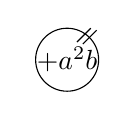
\begin{tikzpicture} \draw (0,0) circle (0.40cm) node {$+a^2b$}; \draw (.20,.20) -- (.375,.375); \draw (.125,.225) -- (.300,.400); \end{tikzpicture}}%
\,\ovalbox{$-2a^3$}%
}{2a^2+4ab+2b^2}$
aequ.
\rule[-3mm]{0pt}{7mm}%
$\displaystyle\frac{2a^2+4ab+2b^2}{2a^2+4ab+2b^2}\;ae$
aequ. \textit{ae}.%
\edlabel{LH_35_09_23_020r_ende_fhg}
\pend%
% \vspace{0.5em}%
\newpage%
%
\pstart%
\noindent%
\lbrack\textit{Nachträglich hinzugefügt und einzeln umrandet:}\rbrack\
\pend%
\vspace{0.5em}%
%
\pstart%
\noindent%
Verum in his errorem esse patet ex reformatione,%
\protect\index{Sachverzeichnis}{reformatio}%
\protect\index{Sachverzeichnis}{error patens ex reformatione}
postquam scilicet deprehendimus aliud esse vim,
aliud quantitatem motus.%
\protect\index{Sachverzeichnis}{quantitas motus}%
\protect\index{Sachverzeichnis}{vis alia a quantitate motus}
\pend%
\vspace{0.5em}%
%
\pstart%
\noindent%
Adjectae hic 
%
\edtext{Tabulae}{%
\lemma{Tabulae}\Cfootnote{%
Die tabellarischen Darstellungen auf
S.~\pageref{LH_35_09_23_017v_tab1}\,f. und
S.~\pageref{LH_35_09_23_018r_tab2}\,f.%
% bzw. \pageref{LH_35_09_23_019r_tab3}f.
}}
%
ex hoc calculo deductae,%
\protect\index{Sachverzeichnis}{tabula a calculo deducta}%
\protect\index{Sachverzeichnis}{calculus}
et experimentis collatae,%
\protect\index{Sachverzeichnis}{tabula experimentis collata}%
\protect\index{Sachverzeichnis}{experimentum}
sed hae nunc aliter
%
\edtext{calculandae.}{%
\lemma{calculandae}\Bfootnote{%
\textit{(1)}~sunt Tabulae 4.
\textit{(2)}~.%
~\textit{L}}}
%
\lbrack59~r\textsuperscript{o}\rbrack\ %    %    %    %    Blatt 59r
%
\pend%
\vspace{2.5em}%
%
%
%%%%    #############################################################
%
%
\pstart%
\noindent%
\lbrack\textit{Nachfolgender Text
(bis zu S.~\refpassage{LH_37_04_060r_tabellenende}{LH_37_04_060r_tabellenende})
ist eine Vorarbeit zu den tabellarischen Darstellungen auf
S.~\pageref{LH_37_05_091r_gestrtab}\,f.,
\pageref{LH_35_09_23_017v_tab1}\,f.,
\pageref{LH_35_09_23_018r_tab2} und
\pageref{LH_35_09_23_019r_tab3}.
% die Bestandteile von N.~\ref{dcc_06-2} %??S01\textsubscript{8} sind.
Der in serifenloser Schrift gesetzte Text ist von Schreiberhand:}\rbrack\
\pend%
\vspace{1.0em}%
% \newpage%
%
\pstart%
\noindent%
\edtext{}{%
{\xxref{LH_059r_ueberschrift_sjw-1}{LH_059r_ueberschrift_sjw-2}}%
\lemma{\textit{Unter der Überschrift:% , umrandet:
}}\Afootnote{\hspace{-1,0mm}%
Experimenta hic proba,%
\protect\index{Sachverzeichnis}{experimentum}
sed non adjectae ratiocinationes.%
\protect\index{Sachverzeichnis}{ratiocinatio}%
% \newline%
}}%
%
\label{37_04_059r_Regnauld_Anfang}%
\hspace{41mm}Schedae%
\protect\index{Sachverzeichnis}{scheda}%
\edlabel{LH_059r_ueberschrift_sjw-1}
secundo-sextae Tabula%
\protect\index{Sachverzeichnis}{tabula}
\textlangle I\textrangle%
%
\hspace{21mm}
Januar. 1678
\pend%
\pstart%
\noindent%
\centering%
\edtext{Experimenta%
\protect\index{Sachverzeichnis}{experimentum}
percussionis%
\protect\index{Sachverzeichnis}{percussio}%
\edlabel{LH_059r_ueberschrift_sjw-2}%
}{%
\lemma{Experimenta percussionis}%
\Cfootnote{%
Siehe
\protect\index{Namensregister}{\textso{Regnauld} (Regnaud; Regnaldus), Fran\c{c}ois de 1626\textendash1689}%
\textsc{F.~Regnauld}, \cite{02021}Brief an B.~de Monconys vom 21.\ Dezember 1655, in: \protect\index{Namensregister}{\textso{Monconys} (Monconisius), Balthasar de 1611\textendash1665}\textsc{B.~de Monconys,} \cite{00118}\title{Journal des voyages}, Teil III: \glqq Lettres escrittes à Monsieur de Monconys\grqq\ (Lyon 1666, S.~52\textendash55, getrennte Paginierung).}}
%
\pend%
\vspace{0.5em}%
%
\pstart%
\noindent%
\edtext{Funependula%
\protect\index{Sachverzeichnis}{funependulum}
duo in diversa ratione.
\newline%
Unum motum alterum
%
\edtext{quiescens.
\newline%
Pondera}{%
\lemma{quiescens.}\Bfootnote{%
\textit{(1)}~ex quibus duo pendebant
\textit{(2)}~. Pondera%
~\textit{L}}}
%
erant globi%
\protect\index{Sachverzeichnis}{globus}
ex ligno%
\protect\index{Sachverzeichnis}{lignum}
duro.%
\edlabel{LH_37_04_059r_regulaeabstr_fnjc-1}%
}{%
\lemma{Funependula \lbrack...\rbrack\ duro}%
\Cfootnote{%
Siehe zu den Versuchsbedingungen a.a.O. (S.~52\,f.).%
\cite{02021}\cite{00118}}}%
%
\edtext{}{%
{\xxref{LH_37_04_059r_regulaeabstr_fnjc-1}{LH_37_04_059r_regulaeabstr_fnjc-2}}%
{\lemma{duro.}\Bfootnote{%
\textit{(1)}~Regulae abstractae
\textit{(a)}~corpus majus incurrens in corpus
\textit{(b)}~Si minus in majus quiescens
\textit{(2)}~Regulae abstractae%
~\textit{L}}}}%
%
%
\pend%
\vspace*{0.5em}%
%
\pstart%
\noindent%
Regulae abstractae%
\protect\index{Sachverzeichnis}{regula abstracta}%
\protect\index{Sachverzeichnis}{regulae concursus corporum}%
\lbrack:\rbrack%
\edlabel{LH_37_04_059r_regulaeabstr_fnjc-2}
% \newline%
$\displaystyle\frac{\epsilon}{e}\ \text{aequ}\ \pleibdashv \displaystyle\frac{b-a}{b}.$\rule[-3mm]{0mm}{0mm}
\newline%
\textit{b} majus,%
\protect\index{Sachverzeichnis}{corpus majus}
% \newline%
\textit{a} minus.%
\protect\index{Sachverzeichnis}{corpus minus}
\newline%
\textit{e} celeritas incursus.%
\protect\index{Sachverzeichnis}{celeritas incursus}
\newline%
$\epsilon$ celeritas incurrentis post concursum.%
\protect\index{Sachverzeichnis}{celeritas incurrentis post concursum}%
\protect\index{Sachverzeichnis}{concursus corporum}
\newline%
Quando majus est incurrens fit \textit{y} aequ. \textit{e}.
\pend%
\vspace{1.0em}%
%
%
\newpage%
%
\pstart%
\noindent%
%
%%%%    Tabelle (16) in (1)%
\label{LH_37_04_059r_tabelle16in1}%
%
\protect\index{Sachverzeichnis}{pendulum descendens}%
\protect\index{Sachverzeichnis}{agens}%
\protect\index{Sachverzeichnis}{patiens}%%
\protect\index{Sachverzeichnis}{descensus penduli}%
\protect\index{Sachverzeichnis}{continuatio penduli}%
\protect\index{Sachverzeichnis}{ascensus penduli}%
\protect\index{Sachverzeichnis}{velocitas descensus}%
\protect\index{Sachverzeichnis}{momentum descensus}%
\protect\index{Sachverzeichnis}{velocitas continuationis}%
\protect\index{Sachverzeichnis}{momentum continuationis}%
\protect\index{Sachverzeichnis}{velocitas ascensus}%
\protect\index{Sachverzeichnis}{momentum ascensus}%
\protect\index{Sachverzeichnis}{vis perdita}%
%
\edtext{%
\hspace*{25mm}(16)\hspace*{27,25mm}descendens in\hspace*{28mm}(1)%
}{\lemma{(16) descendens in (1)}\Cfootnote{%
Vgl. a.a.O. (S.~53).\cite{02021}\cite{00118}
Bei dieser sowie den folgenden tabellarischen Darstellungen sind die jeweiligen Werte der \textit{velocitates} (\textit{descensus}, \textit{continuationis} und \textit{ascensus}) der exzerpierten Vorlage % (Regnaulds Brief an Monconys) 
entnommen.
Die \textit{momenta}, d.h. die Werte der entsprechenden Bewegungsgrößen, sind hingegen von Leibniz bzw. dem Schreiber hinzugerechnet worden.}}%
\newline%
\hspace*{25mm}Agens\hspace*{66,5mm}patiens%
\newline%
\hspace*{25mm}\hspace*{18mm}
velocitates et sub ipsis momenta% \\
% \hspace*{25mm}\hspace*{35mm}momenta%
\newline%
\hspace*{25mm}Descensus\protect\index{Sachverzeichnis}{descensus}\hspace*{5,25mm}Continuationis\protect\index{Sachverzeichnis}{continuatio}\hspace*{5,25mm}Ascensus\protect\index{Sachverzeichnis}{ascensus}\hspace*{7,25mm}Vis perdita\protect\index{Sachverzeichnis}{vis perdita}%
\newline%
\hspace*{25mm}1\hspace*{19mm}$\frac{3}{4}$ fere\hspace*{4,5mm}$(\frac{15}{16})$\hspace*{7,75mm}1$\frac{1}{2}$\hspace{8,75mm}(1)%
\newline%
\scriptsize%
\hspace*{25mm}\hspace*{3mm}16\hspace*{18mm}12\hspace*{26mm}$1\frac{1}{2}$\hspace*{15mm}$2\frac{1}{2}$%
\newline%
\normalsize%
\edtext{%
\hspace*{25mm}2\hspace*{19mm}$1\frac{1}{2}$ plus\hspace*{2mm}$(\frac{30}{16})$\hspace*{8.0mm}3\hspace{10,75mm}(2)%
\newline%
\scriptsize%
\hspace*{25mm}\hspace*{3mm}32\hspace*{18mm}24\hspace*{26mm}3\hspace*{17mm}5%
}{%
\lemma{\textit{Auf der rechten Spalte:}}\Afootnote{%
Nota duplum\textsuperscript{[a]} praecedentis.
\newline\vspace{-0.4em}%
\newline%
{\footnotesize%
\textsuperscript{[a]}~duplum
\textbar~ubique \textit{gestr.}~%
\textbar\ praecedentis%
~\textit{L}}}}%
\newline%
\normalsize%
\hspace*{25mm}3\hspace*{19mm}$2\frac{1}{2}\hspace*{9,5mm}(\frac{45}{16})$\hspace*{8,0mm}4$\frac{1}{5}$\hspace{8,5mm}(3)%
\newline%
\scriptsize%
\hspace*{25mm}\hspace*{3mm}48\hspace*{18mm}40\hspace*{26mm}$4\frac{1}{5}$\hspace*{15mm}$3\frac{4}{5}$%
\newline%
\normalsize%
\hspace*{25mm}4\hspace*{19mm}$3\frac{1}{2}\hspace*{9,5mm}(\frac{60}{16})$\hspace*{8,0mm}6\hspace{10,75mm}(4)%
\newline%
\scriptsize%
\hspace*{25mm}\hspace*{3mm}64\hspace*{18mm}56\hspace*{26mm}6\hspace*{17,125mm}2%
\newline%
\normalsize%
\hspace*{25mm}5\hspace*{19mm}4 plus\hspace*{4,25mm}$(\frac{75}{16})$\hspace*{8,0mm}7 plus\hspace{3,375mm}(5)%
\newline%
\scriptsize%
\hspace*{25mm}\hspace*{3mm}80\hspace*{18mm}64\hspace*{26mm}7\hspace*{17,25mm}9%
\newline%
\normalsize%
\hspace*{25mm}6\hspace*{19mm}5 plus\hspace*{4,25mm}$(\frac{90}{16})$\hspace*{8,125mm}8 plus\hspace{3,363mm}(6)%
\newline%
\scriptsize
\hspace*{25mm}\hspace*{3mm}96\hspace*{18mm}80\hspace*{26mm}8\hspace*{17,25mm}8%
\newline%
\normalsize%
\hspace*{25mm}7\hspace*{19mm}6 plus\hspace*{4,25mm}$(\frac{105}{16})$\hspace*{6,5mm}10 plus\hspace{1,825mm}(7)%
\newline%
\scriptsize%
\hspace*{25mm}\hspace*{2,75mm}112\hspace*{17,0mm}96\hspace*{26mm}10\hspace*{15,75mm}6%
\newline%
\normalsize%
\hspace*{25mm}8\hspace*{19mm}7 plus\hspace*{4,25mm}$(\frac{120}{16})$\hspace*{6,75mm}omissa\hspace{2,375mm}(8)%
\newline%
\scriptsize%
\hspace*{25mm}\hspace*{3,0mm}128\hspace*{17,5mm}112
\pend%
\vspace*{1.5em}
%
\pstart%
\noindent%
\lbrack\textit{Auf der rechten Spalte, neben der vorstehenden Tabelle:}\rbrack\
\pend%
\vspace*{0.5em}
%
\pstart%
\noindent%
Irregularitas%
\protect\index{Sachverzeichnis}{irregularitas progressus virium perditarum}
apparens progressus%
\protect\index{Sachverzeichnis}{progressus virium perditarum}
virium perditarum%
\protect\index{Sachverzeichnis}{vis perdita}
videtur ex eo oriri,
quod
ubi velocitas continuationis%
\protect\index{Sachverzeichnis}{velocitas continuationis}
posita est cum voce\textls{ plus,}
significatur fuisse continuationem%
\protect\index{Sachverzeichnis}{continuatio penduli}
majorem
quam ibi ponitur\lbrack;\rbrack\
quando autem excessus fuit minor dimidio,%
\protect\index{Sachverzeichnis}{excessus continuationis}
tunc notatus non est.
Et \makebox[1.0\textwidth][s]{tamen ob magnitudinem agentis%
\protect\index{Sachverzeichnis}{magnitudo agentis}%
\protect\index{Sachverzeichnis}{agens}%
\lbrack,\rbrack\
magni est momenti% ,
\lbrack:\rbrack\
nam si ponatur fuisse $\displaystyle\frac{1}{4},$
tunc}
\pend
\newpage
\pstart
\noindent vis neglecta%
\protect\index{Sachverzeichnis}{vis neglecta}
erit 4,
ac proinde vis perdita%
\protect\index{Sachverzeichnis}{vis perdita}
revera minor est
quam calculus%
\protect\index{Sachverzeichnis}{calculus}
ostendit.
Nota%
\lbrack:\rbrack\
cum descensus%
\protect\index{Sachverzeichnis}{descensus penduli}
fuit ex 1
tunc continuationem%
\protect\index{Sachverzeichnis}{continuatio penduli}
fuisse%
\textls{ fere }qualis ponitur,
id est paulo minorem:
tunc ergo exceptio paulo ante dicta locum non habet\lbrack,\rbrack\
imo contra deberet vis perdita%
\protect\index{Sachverzeichnis}{vis perdita}
augeri.
Quaeritur,
unde perdita.
Puto
id fieri a parte ictus%
\protect\index{Sachverzeichnis}{ictus receptus}
quam interiores pilae partes%
\protect\index{Sachverzeichnis}{pila penduli}%
\protect\index{Sachverzeichnis}{partes pilae interiores}
in se recipiunt,
item clavus ex quo pendet
\edtext{\lbrack pendulum\rbrack.}{%
\lemma{pendulum}\Bfootnote{\textit{gestr.~L, erg. Hrsg.}}}%
\protect\index{Sachverzeichnis}{pendulum}
\pend%
% \newpage%
\vspace{2.0em}%
%
%
\pstart%
\noindent%
%
%%%%    Tabelle (1) in (16)
%
\label{LH_37_04_059r_tabelle1in16}%
%
\protect\index{Sachverzeichnis}{pendulum descendens}%
\protect\index{Sachverzeichnis}{descensus penduli}%
\protect\index{Sachverzeichnis}{reflexio penduli}%
\protect\index{Sachverzeichnis}{ascensus penduli}%
\protect\index{Sachverzeichnis}{velocitas descensus}%
\protect\index{Sachverzeichnis}{momentum descensus}%
\protect\index{Sachverzeichnis}{velocitas reflexionis}%
\protect\index{Sachverzeichnis}{momentum reflexionis}%
\protect\index{Sachverzeichnis}{velocitas ascensus}%
\protect\index{Sachverzeichnis}{momentum ascensus}%
%
\edtext{%
\hspace*{25mm}(1)\hspace*{12,625mm}descendens in\hspace*{12,5mm}(16)%
}{\lemma{(1) descendens in (16)}\Cfootnote{%
Vgl. a.a.O. (S.~53).\cite{02021}\cite{00118}}}%
\newline%
\hspace*{25mm}Descensus\hspace*{5,25mm}Reflexionis\hspace*{5,625mm}Ascensus%
\newline%
\hspace*{25mm}1\hspace*{18,5mm}$\frac{1}{2}$ plus\hspace*{2,375mm}$(\frac{15}{16})$\hspace*{4,5mm}omissa%
\newline%
\scriptsize%
\hspace*{25mm}\hspace*{3mm}1\hspace*{20mm}$\frac{1}{2}$%
\newline%
\normalsize%
\hspace*{25mm}2\hspace*{19mm}1 plus\hspace*{2,375mm}$(\frac{30}{16})$\hspace*{4,5mm}omissa%
\newline%
\scriptsize%
\hspace*{25mm}\hspace*{3mm}2\hspace*{20mm}1%
\newline%
\normalsize%
\hspace*{25mm}3\hspace*{19mm}$1\frac{1}{2}$\hspace*{7,5mm}$(\frac{45}{16})$\hspace*{4,5mm}\textsf{omissa}%
\newline%
\scriptsize%
\hspace*{25mm}\hspace*{3mm}3\hspace*{20mm}$1\frac{1}{2}$%
\newline%
\normalsize%
\hspace*{25mm}\textsf{4}\hspace*{19,0mm}\textsf{2}\hspace*{9,75mm}$(\frac{60}{16})$\hspace*{4,5mm}\textsf{omissa}%
\newline%
\scriptsize%
\hspace*{25mm}\hspace*{3mm}\textsf{4}\hspace*{20,0mm}\textsf{2}%
\newline%
\normalsize%
\hspace*{25mm}\textsf{5}\hspace*{19mm}\textsf{$\textsf{2}\frac{\textsf{1}}{\textsf{2}}$}\hspace*{7,625mm}$(\frac{75}{16})$\hspace*{4,5mm}\textsf{omissa}%
\newline%
\scriptsize%
\hspace*{25mm}\hspace*{3mm}\textsf{5}\hspace*{20mm}\textsf{2$\frac{1}{2}$}%
\newline%
\normalsize%
\hspace*{25mm}\textsf{6}\hspace*{19mm}\textsf{3}\hspace*{9,75mm}$(\frac{90}{16})$\hspace*{4,5mm}\textsf{omissa}%
\newline%
\scriptsize%
\hspace*{25mm}\hspace*{3mm}\textsf{6}\hspace*{20mm}\textsf{3}%
\newline%
\normalsize%
\hspace*{25mm}\textsf{8}\hspace*{19mm}\textsf{4}\hspace*{9,75mm}$(\frac{120}{16})$\hspace*{3,0mm}\textsf{1}%
\newline%
\scriptsize%
\hspace*{25mm}\hspace*{3mm}\textsf{8}\hspace*{20mm}\textsf{4}%
\normalsize%
% \vspace{0.5em}
\pend%
% \newpage%
%
\vspace*{1.5em}
%
\pstart%
\noindent%
\lbrack\textit{Auf der rechten Spalte, neben der vorstehenden Tabelle:}\rbrack\
\pend%
\vspace*{0.5em}
%
\pstart%
\noindent%
Secundum regulas nostras abstractas%
\protect\index{Sachverzeichnis}{regula abstracta}%
\protect\index{Sachverzeichnis}{regula concursus corporum}
%
\edtext{celeritates continuationis%
\protect\index{Sachverzeichnis}{celeritas continuationis}%
\protect\index{Sachverzeichnis}{continuatio penduli}%
}{%
\lemma{celeritates}\Bfootnote{%
\textit{(1)}~reflexionis
\textit{(2)}~continuationis%
~\textit{L}}}
%
in (16)\,(1)
deberent esse eaedem
cum celeritatibus reflexionis%
\protect\index{Sachverzeichnis}{celeritas reflexionis}%
\protect\index{Sachverzeichnis}{reflexio penduli}
in (1)\,(16).
A quo tamen multum absunt.
\pend%

\pstart%
Item in (16)\,(1)
debet ascensus celeritas%
\protect\index{Sachverzeichnis}{celeritas ascensus}%
\protect\index{Sachverzeichnis}{ascensus penduli}
aequalis esse celeritati descensus.%
\protect\index{Sachverzeichnis}{celeritas descensus}%
\protect\index{Sachverzeichnis}{descensus penduli}
Sed reperitur major.
Semper reperitur.
\pend%
\newpage%
%
%
\pstart%
\noindent%
%
%%%%    Tabelle (8) in (1)
%
\protect\index{Sachverzeichnis}{pendulum descendens}%
\protect\index{Sachverzeichnis}{descensus penduli}%
\protect\index{Sachverzeichnis}{continuatio penduli}%
\protect\index{Sachverzeichnis}{ascensus penduli}%
\protect\index{Sachverzeichnis}{velocitas descensus}%
\protect\index{Sachverzeichnis}{momentum descensus}%
\protect\index{Sachverzeichnis}{velocitas continuationis}%
\protect\index{Sachverzeichnis}{momentum continuationis}%
\protect\index{Sachverzeichnis}{velocitas ascensus}%
\protect\index{Sachverzeichnis}{momentum ascensus}%
%
\edtext{%
\hspace*{25mm}(8)\hspace*{16mm}descendens in\hspace*{16mm}(1)}{%
\lemma{(8) descendens in (1)}\Cfootnote{%
Vgl. a.a.O. (S.~54).\cite{02021}\cite{00118}
Leibniz hat an mehreren Stellen die (der exzerpierten Vorlage getreue) Abschrift des Schreibers durch Streichungen vereinfacht.
Die einzelnen Änderungen von Leibniz werden im textkritischen Variantenapparat nicht ausgewiesen.
Lediglich der endgültige Text wird wiedergegeben.}}%
\label{LH_37_04_059r_tabelle8in1}
\newline%
\textsf{%
\hspace*{25mm}Descensus\hspace*{6,0mm}Continuationis\hspace*{6,75mm}Ascensus%
\newline%
\hspace*{25mm}1}\hspace*{19mm}$(\frac{7}{8})$\hspace{2,5mm}\textsf{0}\hspace*{18,125mm}\textsf{1}\textsf{$\frac{\textsf{1}}{\textsf{2}}$}\hspace{8,75mm}(1)%
\newline%
\scriptsize%
\hspace*{25mm}\hspace*{3mm}\textsf{8}\hspace*{27,5mm}\textsf{0}\hspace*{18,75mm}$ 1 \frac{1}{2}$%
%
\newline%
\normalsize%
\hspace*{25mm}\textsf{2}\hspace*{19mm}$(\frac{14}{8})$\ \textsf{1$\frac{\textsf{1}}{\textsf{2}}$ plus}\hspace*{9mm}\textsf{3 plus}\hspace{3,75mm}(2)%
\newline%
\scriptsize%
\hspace*{25mm}\hspace*{3mm}\textsf{16}\hspace*{26,0mm}\textsf{12}\hspace*{18,0mm}\textsf{3}%
\newline%
\normalsize%
\hspace*{25mm}\textsf{3}\hspace*{19mm}$(\frac{21}{8})$\ \textsf{2$\frac{\textsf{1}}{\textsf{4}}$} % plus
\hspace*{14,75mm}\textsf{5 minus} (3)%
\newline%
\scriptsize%
\hspace*{25mm}\hspace*{3mm}\textsf{24}\hspace*{26,0mm}\textsf{18}\hspace*{18,0mm}\textsf{5}%
\newline%
\normalsize%
\hspace*{25mm}\textsf{4}\hspace*{19mm}$(\frac{28}{8})$\ \textsf{3}\hspace*{18,25mm}\textsf{6 plus}\hspace{3,75mm}(4)%
\newline%
\scriptsize%
\hspace*{25mm}\hspace*{3mm}\textsf{32}\hspace*{26mm}\textsf{24}\hspace*{18,0mm}\textsf{6}%
\newline%
\normalsize%
\hspace*{25mm}\textsf{5}\hspace*{19mm}$(\frac{35}{8})$\ \textsf{4}\hspace*{18,25mm}\textsf{7}\hspace*{3mm}\hspace{7,685mm}(5)%
\newline%
\scriptsize%
\hspace*{25mm}\hspace*{3mm}\textsf{40}\hspace*{26mm}\textsf{32}\hspace*{18,0mm}\textsf{7}%
\newline%
\normalsize%
\hspace*{25mm}\textsf{6}\hspace*{19mm}$(\frac{42}{8})$\ \textsf{$\textsf{4}\frac{\textsf{4}}{\textsf{5}}$} \textsf{plus}\hspace*{9,05mm}\textsf{8 plus}\hspace{3,875mm}(6)%
\newline%
\scriptsize%
\hspace*{25mm}\hspace*{3mm}\textsf{48}\hspace*{26mm}\textsf{$\textsf{38}\frac{\textsf{2}}{\textsf{[5]}}$}\hspace*{15,0mm}\textsf{8}%
\edtext{}{\lemma{\textsf{$\textsf{38}\frac{\textsf{2}}{\textsf{9}}$}}\Bfootnote{\textit{A~ändert Hrsg.}}}%
\newline%
\normalsize%
\hspace*{25mm}\textsf{7}\hspace*{19mm}$(\frac{49}{8})$\ \textsf{$\textsf{5}\frac{\textsf{1}}{\textsf{2}}$} % plus
\hspace*{15mm}\textsf{$\textsf{9}\frac{\textsf{1}}{\textsf{2}}$}\hspace{8,625mm}(7)%
\newline%
\scriptsize%
\hspace*{25mm}\hspace*{3mm}\textsf{56}\hspace*{26,125mm}\textsf{44}\hspace*{18,0mm}\textsf{$\textsf{9}\frac{\textsf{1}}{\textsf{2}}$}%
% }%
\pend%
\newpage%
%
%
\pstart%
\noindent%
%
\lbrack59~v\textsuperscript{o}\rbrack\ %    %    %    %    Blatt 59v
%
\pend%
\vspace{0.5em}%
%
%\pstart%
%\noindent%
%Regulae abstractae\lbrack:\rbrack%
%\edlabel{LH_37_04_059r_regulaeabstr_fnjc-2}
%% \newline%
%$\displaystyle\frac{\epsilon}{e}\ \text{aequ}\ \pleibdashv \displaystyle\frac{b-a}{b}.$\rule[-3mm]{0mm}{0mm}
%\newline%
%\textit{b} majus.
%% \newline%
%\textit{a} minus.
%% \newline%
%\textit{e} celeritas incursus
%% \newline%
%$\epsilon$ celeritas incurrentis post concursum.%
%\protect\index{Sachverzeichnis}{concursus corporum}
%\newline%
%Quando majus est incurrens fit \textit{y} aequ. \textit{e}.
%\pend%
%\vspace{1.0em}%
%%
%\pstart%
%\noindent%
%Irregularitas%
%\protect\index{Sachverzeichnis}{irregularitas}
%apparens progressus virium perditarum%
%\protect\index{Sachverzeichnis}{vis perdita}
%videtur ex eo oriri,
%quod
%ubi velocitas continuationis posita est cum voce\textls{ plus,}
%significatur fuisse continuationem%
%\protect\index{Sachverzeichnis}{continuatio}
%majorem
%quam ibi ponitur\lbrack;\rbrack\
%quando autem excessus fuit minor dimidio,
%tunc notatus non est.
%Ut tamen ob magnitudinem agentis magni est momenti,
%nam si ponatur fuisse $\displaystyle\frac{1}{4}$
%tunc vis neglecta erit 4,
%ac proinde vis perdita revera minor est,
%quam calculus ostendit.
%Nota
%cum descensus fuit ex 1
%tunc continuationem fuisse%
%\textls{ fere }%
%qualis ponitur,
%id est paulo minorem:
%tunc ergo exceptio paulo ante dicta locum non habet\lbrack,\rbrack\
%imo contra deberet vis perdita%
%\protect\index{Sachverzeichnis}{vis perdita}
%augeri.
%Quaeritur,
%unde perdita.
%Puto
%id fieri a parte ictus
%quam interiores pilae partes in se recipiunt,
%item clavus ex quo pendet pendulum.
%\pend%
%
%\pstart%
%Secundum regulas nostras abstractas
%
%\edtext{celeritates continuationis%
%\protect\index{Sachverzeichnis}{celeritas continuationis}%
%}{%
%\lemma{celeritates}\Bfootnote{%
%\textit{(1)}~reflexionis
%\textit{(2)}~continuationis%
%~\textit{L}}}
%
%in (16)\,(1) deberent esse eaedem cum celeritatibus reflexionis in (1)\,(16).
%A quo tamen multum absunt.
%\pend%
%
%\pstart%
%Item in (16)\,(1) debet ascensus celeritas aequalis esse celeritati descensus.
%Sed reperitur major.
%Semper reperitur.
%\pend%
%
%\pstart%
%\noindent%
%Excessus celeritatis ascensus%
%\protect\index{Sachverzeichnis}{ascensus}
%in incursu majoris in minus
%crescit super eum
%qui deberet esse
%seu super descensum majoris;
%cum ipso descensu crescent ita
%ut quanto celeritas est major,
%tanto aberratio\protect\index{Sachverzeichnis}{aberratio}
%%
%\edtext{\lbrack fit\rbrack}{%
%\lemma{sit}\Bfootnote{%
%textit{L~ändert Hrsg.}}}
%%
%major,
%seu excessus ascensus super descensum.
%Iisdem positis corporibus.
%\pend%
%%
%\pstart%
%Iisdem manentibus celeritatibus
%et corporibus incurrentibus
%seu majoribus versus aequalitatem decrescentibus
%etiam differentia seu excessus ascensuum
%super descensus\protect\index{Sachverzeichnis}{descensus}
%decrescit.
%Verbi gratia
%\newline%
%\hspace*{7,5mm}descensus 7
%\hspace*{5mm}corpora (16) (1)
%\hspace*{5mm}ascensus 10 plus\\ 
%\hspace*{44,5mm}(8)\hspace*{28mm}9 1/2\\
%\hspace*{44,5mm}(4)\hspace*{28mm}9\\
%\hspace*{7,5mm}descensus 5
%\hspace*{5mm}corpora (16) (1)
%\hspace*{5mm}ascensus 7 plus\\
%\hspace*{44,5mm}(8)\hspace*{28mm}7\\
%\hspace*{44,5mm}(4)\hspace*{28mm}6$\frac{1}{4}$\\
%\hspace*{44,5mm}(2)\hspace*{28mm}5 plus\\
%\hspace*{44,5mm}(1)\hspace*{28mm}4
%\newline%
%ubi tamen puto in ultimo (1), 4
%%
%\edtext{esse difficultatem,}{%
%\lemma{esse}\Bfootnote{%
%\textit{(1)}~errorem,
%\textit{(2)}~difficultatem,%
%~\textit{L}}}
%%
%nunquam enim alias fit minor quam descensus.
%Errorem%
%\protect\index{Sachverzeichnis}{error}
%tamen esse dicere non audeo,
%quia
%semper ubi incurrit 1 in 1
%video semper ascensum fieri minorem descensu.%
%\protect\index{Sachverzeichnis}{descensus}
%%
%\pend%
%%
%\pstart%
%Ante omnia necesse est
%aliquod ex vi perire
%quia pendulum ne liberum quidem est solum
%nec impeditum
%%
%\edtext{\lbrack unquam\rbrack}{%
%\lemma{nunquam}\Bfootnote{%
%\textit{L~ändert Hrsg.}}}
%%
%tam alte ascendit
%quam descenderat.
%Deinde ea
%quae cum globis ligneis eveniunt,
%quodammodo media esse debent inter ea
%quae evenirent cum mollibus argillaceis
%et cum chalybeis durissimis.
%V.g. cum (8) descendit in (1),
%continuatio ipsius (8),
%et ascensus ipsius (1)
%erit unumquodque
%$\displaystyle\frac{8}{9}, \frac{16}{9}, \frac{24}{9}$ etc.
%prout ex 1, 2, 3 etc. descendit.
%Si scl. globi sint argillacei.
%Si vero sint durissimi erit continuatio
%$\displaystyle\frac{7}{8}, \frac{14}{8}, \frac{21}{8}$ etc.
%ascensus vero 1, 2, 3.
%\pend%
%%
%\pstart%
%Si medii minuitur continuatio%
%\protect\index{Sachverzeichnis}{continuatio}
%augetur ascensus.%
%\protect\index{Sachverzeichnis}{ascensus}
%Quod vid\textlangle etur\textrangle\ absurdum.
%Nam differentia continu\textlangle atio\textrangle nis
%ab asce\textlangle nsu\textrangle\
%\textlangle dependit\textrangle\
%a quant\textlangle itate\textrangle\ \textlangle...\textrangle\
%\textlangle qu\textrangle\ ae utique in
%\textlangle...\textrangle\
%major.
%Hinc ergo colligo%
%\lbrack:\rbrack\
%si experimenta%
%\protect\index{Sachverzeichnis}{experimentum}
%%
%\edtext{ista accurata}{%
%\lemma{ista}\Bfootnote{%
%\textit{(1)}~vera
%\textit{(2)}~accurata%
%~\textit{L}}}
%%
%sunt,
%de quo non dubito
%%
%\edtext{(\protect\vphantom)%
%quia consentiunt inter se,
%et deceptio%
%\protect\index{Sachverzeichnis}{deceptio}
%et virium deperditio%
%\protect\index{Sachverzeichnis}{deperditio virium}
%hic nil obstat
%quia minueret potius
%quam augeret ascensum%
%\protect\vphantom(),}{%
%\lemma{(\protect\vphantom)quia}\Bfootnote{%
%\hspace{-0,5mm}consentiunt \lbrack...\rbrack\ augeret ascensum\protect\vphantom() \textit{erg.}%
%~\textit{L}}}
%%
%falsam esse opinionem%
%\textls{ (}\vphantom)%
%\textls{quod
%si majus incurrat in minus ascendens
%in durissimis aequetur ascensus descensui}%
%\vphantom(\textls{);}
%sed potius fieri debet major\lbrack,\rbrack\
%inprimis cum experimenta haec ostendant,
%eo majorem fieri,
%quo magis augetur percussio,%
%\protect\index{Sachverzeichnis}{percussio aucta}
%quod fit,
%quo major est celeritas.
%%
%\lbrack59~v\textsuperscript{o}\rbrack\ %    %    %    %    Blatt 59v
%%
%\pend%
%\vspace*{1em}%
%\newpage%
%
\pstart%
\noindent%
%
%%%%    Tabelle (1) in (8)
%
\protect\index{Sachverzeichnis}{pendulum descendens}%
\protect\index{Sachverzeichnis}{descensus penduli}%
\protect\index{Sachverzeichnis}{reflexio penduli}%
\protect\index{Sachverzeichnis}{ascensus penduli}%
\protect\index{Sachverzeichnis}{velocitas descensus}%
\protect\index{Sachverzeichnis}{momentum descensus}%
\protect\index{Sachverzeichnis}{velocitas reflexionis}%
\protect\index{Sachverzeichnis}{momentum reflexionis}%
\protect\index{Sachverzeichnis}{velocitas ascensus}%
\protect\index{Sachverzeichnis}{momentum ascensus}%
%
\textsf{%
\edtext{%
\hspace*{25mm}(1)\hspace*{15mm}descendens in\hspace*{15mm}(8)%
}{\lemma{(1) descendens in (8)}\Cfootnote{%
Vgl. a.a.O. (S.~54).\cite{02021}\cite{00118}
Leibniz hat an mehreren Stellen die (der exzerpierten Vorlage getreue) Abschrift des Schreibers durch Streichungen vereinfacht.
Die einzelnen Änderungen von Leibniz werden im textkritischen Variantenapparat nicht ausgewiesen.
Lediglich der endgültige Text wird wiedergegeben.%
}}%
\newline%
\hspace*{25mm}Descensus\hspace*{7mm}Reflexionis\hspace*{8,5mm}Ascensus%
\newline%
\hspace*{25mm}2\hspace*{20,25mm}1 plus\hspace*{15mm}0%
\newline%
\scriptsize%
\hspace*{25mm}\hspace*{3mm}2\hspace*{20,5mm}1%
\newline%
\normalsize%
\hspace*{25mm}3\hspace*{20,25mm}$\textsf{1}\frac{\textsf{1}}{\textsf{2}}$\hspace*{16mm}%
\newline%
\scriptsize%
\hspace*{25mm}\hspace*{3mm}3\hspace*{20,5mm}$\textsf{1}\frac{\textsf{1}}{\textsf{2}}$%
\newline%
\normalsize%
\hspace*{25mm}4\hspace*{20,25mm}2 minus%
\newline%
\scriptsize%
\hspace*{25mm}\hspace*{3mm}4\hspace*{20,5mm}2%
\newline%
\normalsize%
\hspace*{25mm}5\hspace*{20,25mm}2 plus\hspace*{15mm}\edtext{[1]}{%
\lemma{\textsf{1 0}}\Bfootnote{\textit{A~ändert Hrsg.}}} min.%
\newline%
\scriptsize%
\hspace*{25mm}\hspace*{3mm}5\hspace*{20,5mm}2%
\newline%
\normalsize%
\hspace*{25mm}6\hspace*{20,25mm}$\textsf{2}\frac{\textsf{1}}{\textsf{2}}$\hspace*{19,875mm}$\textsf{1}\frac{\textsf{1}}{\textsf{4}}$%
\newline%
\scriptsize%
\hspace*{25mm}\hspace*{3mm}6\hspace*{20,5mm}$\textsf{2}\frac{\textsf{1}}{\textsf{2}}$\hspace*{19,875mm}10%
\newline%
\normalsize%
\hspace*{25mm}7\hspace*{20,25mm}3\hspace*{22,125mm}$\textsf{1}\frac{\textsf{1}}{\textsf{3}}$%
\newline%
\scriptsize%
\hspace*{25mm}\hspace*{3mm}7\hspace*{20,5mm}3\hspace*{21,75mm}$\textsf{10}\frac{\textsf{2}}{\textsf{3}}$%
\newline%
\normalsize%
\hspace*{25mm}8\hspace*{20,25mm}3 plus\hspace*{15,5mm}omissa%
\newline%
\scriptsize%
\hspace*{25mm}\hspace*{3mm}8\hspace*{20,5mm}3%
\newline%
\normalsize%
\hspace*{25mm}10\hspace*{18,75mm}4\hspace*{22mm}$\textsf{1}\frac{\textsf{1}}{\textsf{2}}$%
\newline%
\scriptsize%
\hspace*{25mm}\hspace*{3mm}10\hspace*{19,25mm}4\hspace*{21,75mm}12}
\pend%
%\vspace*{1em}%
\newpage%
%
%
\pstart%
\noindent%
%
%%%%    Tabelle (4) in (1)
%
\protect\index{Sachverzeichnis}{pendulum descendens}%
\protect\index{Sachverzeichnis}{descensus penduli}%
\protect\index{Sachverzeichnis}{continuatio penduli}%
\protect\index{Sachverzeichnis}{ascensus penduli}%
\protect\index{Sachverzeichnis}{velocitas descensus}%
\protect\index{Sachverzeichnis}{momentum descensus}%
\protect\index{Sachverzeichnis}{velocitas continuationis}%
\protect\index{Sachverzeichnis}{momentum continuationis}%
\protect\index{Sachverzeichnis}{velocitas ascensus}%
\protect\index{Sachverzeichnis}{momentum ascensus}%
%
% \newline%
\textsf{%
\edtext{%
\hspace*{25mm}(4)\hspace*{17,5mm}descendens in\hspace*{17,5mm}(1)}{%
\lemma{(4) descendens in (1)}\Cfootnote{%
Vgl. a.a.O. (S.~54).\cite{02021}\cite{00118}
Leibniz hat an mehreren Stellen die (der exzerpierten Vorlage getreue) Abschrift des Schreibers durch Streichungen vereinfacht.
Die einzelnen Änderungen von Leibniz werden im textkritischen Variantenapparat nicht ausgewiesen.
Lediglich der endgültige Text wird wiedergegeben.%
}}%
\newline%
\hspace*{25mm}Descensus\hspace*{7mm}Continuationis\hspace*{8,0mm}Ascensus%
\newline%
\hspace*{25mm}1\hspace*{20,25mm}0\hspace*{3mm}0\hspace*{22,375mm}$\textsf{1}\frac{\textsf{1}}{\textsf{2}}$%
\newline%
\scriptsize%
\hspace*{25mm}\hspace*{3mm}4\hspace*{20,5mm}0\hspace*{3,25mm}0\hspace{24mm}$\textsf{1}\frac{\textsf{1}}{\textsf{2}}$%
\newline%
\normalsize%
\hspace*{25mm}2\hspace*{20,25mm}1\hspace*{27,25mm}$\textsf{2}\frac{\textsf{3}}{\textsf{5}}$%
\newline%
\scriptsize%
\hspace*{25mm}\hspace*{3mm}8\hspace*{20,5mm}4\hspace*{28,75mm}$\textsf{2}\frac{\textsf{3}}{\textsf{5}}$%
\newline%
\normalsize%
\hspace*{25mm}3\hspace*{20,25mm}2 minus\hspace*{17,5mm}4%
\newline%
\scriptsize%
\hspace*{25mm}\hspace*{3mm}12\hspace*{19,25mm}8\hspace*{28,625mm}4%
\newline%
\normalsize%
\hspace*{25mm}4\hspace*{20,25mm}$\textsf{2}\frac{\textsf{1}}{\textsf{2}}$ minus\hspace*{15,25mm}$\textsf{5}\frac{\textsf{1}}{\textsf{2}}$ plus%
\newline%
\scriptsize%
\hspace*{25mm}\hspace*{3mm}16\hspace*{19,25mm}10\hspace*{27,25mm}$\textsf{5}\frac{\textsf{1}}{\textsf{2}}$%
\newline%
\normalsize%
\hspace*{25mm}$\textsf{4}\frac{\textsf{1}}{\textsf{2}}$\hspace*{18mm}$\textsf{2}\frac{\textsf{1}}{\textsf{2}}$\hspace*{25,25mm}6%
\newline%
\scriptsize%
\hspace*{25mm}\hspace*{3mm}18\hspace*{19,25mm}10\hspace*{27,25mm}6%
\newline%
\normalsize%
\hspace*{25mm}5\hspace*{20,25mm}3\hspace*{27,25mm}$\textsf{6}\frac{\textsf{1}}{\textsf{4}}$%
\newline%
\scriptsize%
\hspace*{25mm}\hspace*{3mm}20\hspace*{19,25mm}12\hspace*{27,25mm}$\textsf{6}\frac{\textsf{1}}{\textsf{4}}$%
\newline%
\normalsize%
\hspace*{25mm}6\hspace*{20,25mm}4\hspace*{27,25mm}$\textsf{7}\frac{\textsf{3}}{\textsf{4}}$%
\newline%
\scriptsize%
\hspace*{25mm}\hspace*{3mm}24\hspace*{19,25mm}16\hspace*{27,25mm}$\textsf{7}\frac{\textsf{3}}{\textsf{4}}$%
\newline%
\normalsize%
\hspace*{25mm}7\hspace*{20,25mm}$\textsf{4}\frac{\textsf{2}}{\textsf{5}}$\hspace*{25,125mm}9%
\newline%
\scriptsize%
\hspace*{25mm}\hspace*{3mm}28\hspace*{19,25mm}$\textsf{17}\frac{\textsf{3}}{\textsf{5}}$\hspace*{25,5mm}9%
\newline%
\normalsize%
\hspace*{25mm}8\hspace*{20,25mm}[5\hspace*{26,0mm}10]%
\edtext{}{\lemma{5\ 1\quad 0}\Bfootnote{\textit{A~ändert Hrsg.}}}%
\newline%
\scriptsize%
\hspace*{25mm}\hspace*{3mm}32\hspace*{19,25mm}[20\hspace*{26,5mm}10]%
\edtext{}{\lemma{20\ 4\quad 0}\Bfootnote{\textit{A~ändert Hrsg.}}}%
\newline%
\normalsize%
\hspace*{25mm}9\hspace*{20,25mm}6\hspace*{27,25mm}omissa%
\newline%
\scriptsize%
\hspace*{25mm}\hspace*{3mm}36\hspace*{19,25mm}24%
}%
\normalsize%
\pend%
\vspace{1.5em}%
%
%
\pstart%
\noindent%
\lbrack\textit{Auf der linken Spalte, % von Bl.~59~v\textsuperscript{o}, 
neben der vorstehenden Tabelle:}\rbrack\
\pend%
\vspace{0.5em}%
%
\pstart%
\noindent%
\textlangle Cu\textrangle m descensus celeritas%
\protect\index{Sachverzeichnis}{celeritas descensus}
est $4\frac{1}{2},$
celeritas ascensus%
\protect\index{Sachverzeichnis}{celeritas ascensus}
est 6
\textlangle e\textrangle t excessus%
\protect\index{Sachverzeichnis}{excessus celeritatis ascensus}
est $1\frac{1}{2}.$
\pend%
\vspace{0.5em}%
%
\pstart%
\noindent%
\textlangle Cu\textrangle m celeritas descensus%
\protect\index{Sachverzeichnis}{celeritas descensus}
est 5,
celeritas ascensus%
\protect\index{Sachverzeichnis}{celeritas ascensus}
est $6\frac{1}{4}$
et tunc excessus est $1\frac{1}{4},$
minor quam ante\lbrack;\rbrack\
in quo puto aliquis error,\protect\index{Sachverzeichnis}{error}
nam alias semper video crescere excessus.%
\protect\index{Sachverzeichnis}{excessus celeritatis ascensus}
% \newline%
\pend%
\newpage%
%
\pstart%
\noindent%
%
%%%%    Tabelle (1) in (4)
%
\protect\index{Sachverzeichnis}{pendulum descendens}%
\protect\index{Sachverzeichnis}{descensus penduli}%
\protect\index{Sachverzeichnis}{reflexio penduli}%
\protect\index{Sachverzeichnis}{ascensus penduli}%
\protect\index{Sachverzeichnis}{velocitas descensus}%
\protect\index{Sachverzeichnis}{momentum descensus}%
\protect\index{Sachverzeichnis}{velocitas reflexionis}%
\protect\index{Sachverzeichnis}{momentum reflexionis}%
\protect\index{Sachverzeichnis}{velocitas ascensus}%
\protect\index{Sachverzeichnis}{momentum ascensus}%
%
\label{LH_37_04_059v_Tab(1)in(4)}%
\textsf{%
\edtext{%
\hspace*{25mm}(1)\hspace*{15mm}descendens in\hspace*{15mm}(4)%
}{\lemma{(1) descendens in (4)}\Cfootnote{%
Vgl. a.a.O. (S.~54).\cite{02021}\cite{00118}
Leibniz hat an mehreren Stellen die (der exzerpierten Vorlage getreue) Abschrift des Schreibers durch Streichungen vereinfacht.
Die einzelnen Änderungen von Leibniz werden im textkritischen Variantenapparat nicht ausgewiesen.
Lediglich der endgültige Text wird wiedergegeben.%
%\hfill%
}}%
\newline%
\hspace*{25mm}Descensus\hspace*{7mm}Reflexionis\hspace*{8,25mm}Ascensus%
\newline%
\hspace*{25mm}3\hspace*{20mm}1 minus\hspace*{12,125mm}1%
\newline%
\scriptsize
\hspace*{25mm}\hspace*{3mm}3\hspace*{20mm}1\hspace{23,0mm}4%
\newline%
\normalsize
\hspace*{25mm}4\hspace*{20mm}1\hspace*{21,875mm}\textsf{$\textsf{1}\frac{\textsf{1}}{\textsf{4}}$}%
\newline%
\scriptsize
\hspace*{25mm}\hspace*{3mm}4\hspace*{20mm}1\hspace*{23,0mm}5%
\newline%
\normalsize
\hspace*{25mm}6\hspace*{20mm}2\hspace*{22,0mm}2%
\newline%
\scriptsize
\hspace*{25mm}\hspace*{3mm}6\hspace*{20mm}2\hspace*{23,0mm}8%
\newline%
\normalsize
\hspace*{25mm}8\hspace*{20mm}2 plus\hspace*{15,0mm}\textsf{$\textsf{2}\frac{\textsf{1}}{\textsf{3}}$}%
\newline%
\scriptsize
\hspace*{25mm}\hspace*{3mm}8\hspace*{20mm}2\hspace*{23,0mm}\textsf{$\textsf{9}\frac{\textsf{1}}{\textsf{3}}$}%
\newline%
\normalsize
\hspace*{25mm}9\hspace*{20mm}3\hspace*{22,0mm}3%
\newline%
\scriptsize
\hspace*{25mm}\hspace*{3mm}9\hspace*{20mm}3\hspace*{23,0mm}12%
}%
\normalsize
\pend%
\vspace*{1.0em}
% \newpage%
%
\pstart%
\noindent%
%
\lbrack60~r\textsuperscript{o}\rbrack\ %    %    %    %    Blatt 60r
%
\pend%
\vspace{0.5em}
% \newpage%
%
\pstart%
\noindent%
%
%%%%    Tabelle (2) in (1)
%
\protect\index{Sachverzeichnis}{pendulum descendens}%
\protect\index{Sachverzeichnis}{descensus penduli}%
\protect\index{Sachverzeichnis}{continuatio penduli}%
\protect\index{Sachverzeichnis}{ascensus penduli}%
\protect\index{Sachverzeichnis}{velocitas descensus}%
\protect\index{Sachverzeichnis}{momentum descensus}%
\protect\index{Sachverzeichnis}{velocitas continuationis}%
\protect\index{Sachverzeichnis}{momentum continuationis}%
\protect\index{Sachverzeichnis}{velocitas ascensus}%
\protect\index{Sachverzeichnis}{momentum ascensus}%
%
\textsf{%
\edtext{%
\hspace*{25mm}(2)\hspace*{17,5mm}descendens in\hspace*{17,5mm}(1)}{%
\lemma{(2) descendens in (1)}%
\Cfootnote{%
Vgl. a.a.O. (S.~55).\cite{02021}\cite{00118}%
% \hfill%
}}%
\newline%
\hspace*{25mm}Descensus\hspace*{7,0mm}Continuationis\hspace*{8,0mm}Ascensus%
\newline%
\hspace*{25mm}5\hspace*{20,25mm}2 minus\hspace*{17,5mm}5 plus%
\newline%
\scriptsize
\hspace*{25mm}\hspace*{3mm}10\hspace*{19,5mm}4\hspace{27,75mm}5%
\newline%
\normalsize
\hspace*{25mm}6\hspace*{20,25mm}2\hspace{3,0mm}0\hspace*{22,5mm}6 plus%
\newline%
\scriptsize
\hspace*{25mm}\hspace*{3mm}12\hspace*{19,5mm}4\hspace*{27,75mm}6%
\newline%
\normalsize
\hspace*{25mm}8\hspace*{20,25mm}\textsf{$\textsf{3}\frac{\textsf{1}}{\textsf{4}}$}\hspace*{25,125mm}8\hspace{3,0mm}0%
\newline%
\scriptsize
\hspace*{25mm}\hspace*{3mm}16\hspace*{19,5mm}\textsf{$\textsf{6}\frac{\textsf{2}}{\textsf{4}}$}\hspace*{26mm}8%
}%
\normalsize%
\pend%
\vspace{1.5em}%
%\newpage%
%
%
\pstart%
\noindent%
%
%%%%    Tabelle (1) in (2)
%
\protect\index{Sachverzeichnis}{pendulum descendens}%
\protect\index{Sachverzeichnis}{descensus penduli}%
\protect\index{Sachverzeichnis}{reflexio penduli}%
\protect\index{Sachverzeichnis}{continuatio penduli}%
\protect\index{Sachverzeichnis}{ascensus penduli}%
\protect\index{Sachverzeichnis}{velocitas descensus}%
\protect\index{Sachverzeichnis}{momentum descensus}%
\protect\index{Sachverzeichnis}{velocitas reflexionis}%
\protect\index{Sachverzeichnis}{velocitas continuationis}%
\protect\index{Sachverzeichnis}{momentum reflexionis}%
\protect\index{Sachverzeichnis}{momentum continuationis}%
\protect\index{Sachverzeichnis}{velocitas ascensus}%
\protect\index{Sachverzeichnis}{momentum ascensus}%
%
\textsf{%
\hspace*{25mm}(1)\hspace*{17,5mm}descendens in\hspace*{17,5mm}(\vphantom)}%
%
\edtext{2}{%
\lemma{\textsf{in (\protect\vphantom)}}\Bfootnote{%
\textit{(1)}~\textsf{1}~\textit{A}
\textit{(2)}~2%
~\textit{LiA}}}%
%
\textsf{\vphantom()%
\edtext{}{\lemma{\textsf{(1) descendens in (2)}}\Cfootnote{%
Vgl. a.a.O. (S.~55).\cite{02021}\cite{00118}
Die exzerpierte Vorlage gibt irrtümlich \textit{1 descendens in 1} an.
Daher verbessert Leibniz, wie im textkritischen Variantenapparat ausgewiesen, die (an sich getreue) Abschrift des Schreibers.}}%
\newline%
\hspace*{25mm}Descensus\hspace*{6,75mm}Non fuit obser-\hspace*{6,75mm}Ascensus%
\newline%
\hspace*{34mm}vata nec continuatio nec reflexio%
\newline%
\hspace*{25mm}8\hspace*{20,25mm}0\hspace{3,0mm}0\hspace*{22,125mm}4%
\newline%
\scriptsize%
\hspace*{25mm}\hspace*{3mm}8\hspace{50,0mm}%
}%
\scriptsize%
8\edtext{}{%
\lemma{\textsf{8}}\Bfootnote{%
\textit{(1)}~\textsf{4}~\textit{A}
\textit{(2)}~8%
~\textit{LiA}}}%
%
\normalsize%
\pend%
\newpage
%\vspace*{1.0em}%
%
%
\pstart%
\noindent%
\lbrack\textit{Auf der linken Spalte, % von Bl.~60~r\textsuperscript{o}, 
neben der vorstehenden Tabelle:}\rbrack\
\pend%
\vspace{0.5em}%
%
%
\pstart%
\noindent%
Hic puto nonnihil erratum in observando%
\protect\index{Sachverzeichnis}{erratum in observando}%
\lbrack,\rbrack\
cum enim in caeteris casibus omnibus%
\protect\index{Sachverzeichnis}{casus}
aliquid de vi perdatur.%
\protect\index{Sachverzeichnis}{vis perdita}
%
\edtext{Cur in hoc solo nihil.}{%
\lemma{Cur}\Bfootnote{%
\textit{(1)}~non
\textit{(2)}~in hoc solo nihil.%
~\textit{L}}}
\pend%
\vspace{1.5em}%
% \newpage%
%
%
\pstart%
\noindent%
%
%%%%    Tabelle (1) in (1)
%
\label{LH_37_04_060r_tabelle1in1}%
%
\protect\index{Sachverzeichnis}{pendulum descendens}%
\protect\index{Sachverzeichnis}{descensus penduli}%
\protect\index{Sachverzeichnis}{continuatio penduli}%
\protect\index{Sachverzeichnis}{ascensus penduli}%
\protect\index{Sachverzeichnis}{velocitas descensus}%
\protect\index{Sachverzeichnis}{momentum descensus}%
\protect\index{Sachverzeichnis}{velocitas continuationis}%
\protect\index{Sachverzeichnis}{momentum continuationis}%
\protect\index{Sachverzeichnis}{velocitas ascensus}%
\protect\index{Sachverzeichnis}{momentum ascensus}%
%
\textsf{%
\edtext{%
\hspace*{25mm}(1)\hspace*{17,5mm}descendens in\hspace*{17,5mm}(1)}{%
\lemma{(1) descendens in (1)}\Cfootnote{%
Vgl. a.a.O. (S.~55).\cite{02021}\cite{00118}}}%
\newline%
\hspace*{25mm}Descensus\hspace*{7,0mm}Continuationis\hspace*{7,625mm}Ascensus%
\newline%
\hspace*{25mm}2\hspace*{20,25mm}0 plus\hspace*{19,625mm}\textsf{$\textsf{1}\frac{\textsf{3}}{\textsf{4}}$}%
\newline%
\scriptsize%
\hspace*{25mm}\hspace*{3mm}2\hspace*{20,875mm}0\hspace{29,0mm}\textsf{$\textsf{1}\frac{\textsf{3}}{\textsf{4}}$}%
\newline%
\normalsize%
\hspace*{25mm}4\hspace*{20,25mm}0 plus\hspace*{19,625mm}\textsf{$\textsf{3}\frac{\textsf{1}}{\textsf{2}}$}%
\newline%
\scriptsize%
\hspace*{25mm}\hspace*{3mm}4\hspace*{20,875mm}0\hspace{29,125mm}\textsf{$\textsf{3}\frac{\textsf{1}}{\textsf{2}}$}%
\newline%
\normalsize%
\hspace*{25mm}5\hspace*{20,25mm}0 plus\hspace*{19,625mm}4%
\newline%
\scriptsize%
\hspace*{25mm}\hspace*{3mm}5\hspace*{20,875mm}0\hspace{29,25mm}4%
\newline%
\normalsize%
\hspace*{25mm}8\hspace*{20,25mm}1 minus\hspace*{16,75mm}6%
\newline%
\scriptsize%
\hspace*{25mm}\hspace*{3mm}8\hspace*{20,875mm}1\hspace{29,25mm}6%
%
}%
\normalsize%
\pend%
% \newpage%
\vspace{1.0em}%
%
%
\pstart%
\noindent%
\lbrack\textit{Auf der linken Spalte, % von Bl.~60~r\textsuperscript{o}, 
neben der vorstehenden Tabelle:}\rbrack%
\pend%
\vspace{0.5em}%
%
\pstart%
\noindent%
Miror in casu aequalitatis%
\protect\index{Sachverzeichnis}{casus aequalitatis corporum}
minorem fieri ascensum decensu.%
\protect\index{Sachverzeichnis}{ascensus penduli}%
\protect\index{Sachverzeichnis}{descensus penduli}
Imo jam video rationem,
quia necessario aliquid de vi perditur%
\protect\index{Sachverzeichnis}{vis perdita}%
\lbrack;\rbrack\
ideo non potest esse aequalis.
Major autem omnino esse non potest,
alioqui augeretur tota vis.%
\protect\index{Sachverzeichnis}{vis tota}%
\protect\index{Sachverzeichnis}{vis aucta}
Accidit quod aliquis semper motus fuit in incurrente superstes,%
\protect\index{Sachverzeichnis}{motus incurrentis superstes}
qui haud dubie oritur ex imperfectione Elateris,%
\protect\index{Sachverzeichnis}{imperfectio elateris}%
\protect\index{Sachverzeichnis}{elater}
in quantum scil.
duo corpora pro mollibus%
\protect\index{Sachverzeichnis}{corpus molle}
haberi possunt.
%
\lbrack59~r\textsuperscript{o}\rbrack\ %    %    %    %    Blatt 59r
%
\pend%
\vspace{1.5em}%
%\newpage%
%
%
\pstart%
\noindent%
\lbrack\textit{Auf der rechten Spalte von Bl.~59~r\textsuperscript{o}% , fortgesetzt auf der linken Spalte von Bl.~60~r\textsuperscript{o}
\!:}\rbrack\
\pend%
\vspace{0.5em}%
%
\pstart%
\noindent%
%%
%\lbrack59~r\textsuperscript{o}\rbrack\ %    %    %    %    Blatt 59r
%%
Excessus celeritatis ascensus%
\protect\index{Sachverzeichnis}{excessus celeritatis ascensus}%
\protect\index{Sachverzeichnis}{celeritas ascensus}%
\protect\index{Sachverzeichnis}{ascensus penduli}
in incursu majoris in minus%
\protect\index{Sachverzeichnis}{incursus majoris in minus}%
\protect\index{Sachverzeichnis}{corpus majus in minus}
crescit super eum
qui deberet esse%
\lbrack,\rbrack\
seu super descensum majoris% ;%
\protect\index{Sachverzeichnis}{descensus corporis majoris}%
\lbrack,\rbrack\
cum ipso descensu%
\protect\index{Sachverzeichnis}{descensus penduli}
%
crescen\textlangle te\textrangle,
%\edtext{\lbrack crescit\rbrack,}{%
%\lemma{crescen\textlangle t\textrangle}\Bfootnote{%
%\textit{L~ändert Hrsg.}}}
%
ita ut quanto celeritas est major,%
\protect\index{Sachverzeichnis}{celeritas descensus}
tanto aberratio\protect\index{Sachverzeichnis}{aberratio}
%
sit
%\edtext{\lbrack fit\rbrack}{%
%\lemma{}\Bfootnote{%
%\textit{L~ändert Hrsg.}}}
%
major,
seu excessus ascensus super descensum.%
\protect\index{Sachverzeichnis}{excessus ascensus super descensum}%
\protect\index{Sachverzeichnis}{ascensus penduli}%
\protect\index{Sachverzeichnis}{descensus penduli}
Iisdem positis corporibus.
\pend%
%
\pstart%
Iisdem manentibus celeritatibus,%
\protect\index{Sachverzeichnis}{celeritas descensus}
et corporibus incurrentibus%
\protect\index{Sachverzeichnis}{corpus incurrens}
seu majoribus versus aequalitatem decrescentibus,%
\protect\index{Sachverzeichnis}{aequalitas corporum concurrentium}
etiam differentia seu excessus ascensuum%
\protect\index{Sachverzeichnis}{excessus ascensus super descensum}%
\protect\index{Sachverzeichnis}{ascensus penduli}
super descensus\protect\index{Sachverzeichnis}{descensus penduli}
decrescit.
Verbi gratia
\pend
\newpage
\pstart\noindent
%\newline%
\hspace*{7,5mm}descensus 7
\hspace*{5mm}corpora (16) (1)
\hspace*{5mm}ascensus 10 plus\\ 
\hspace*{44,5mm}(8)\hspace*{28mm}9 1/2\\
\hspace*{44,5mm}(4)\hspace*{28mm}9\\
\hspace*{7,5mm}descensus 5
\hspace*{5mm}corpora (16) (1)
\hspace*{5mm}ascensus\: 7 plus\\
\hspace*{44,5mm}(8)\hspace*{28mm}7\\
\hspace*{44,5mm}(4)\hspace*{28mm}6$\frac{1}{4}$\\
\hspace*{44,5mm}(2)\hspace*{28mm}5 plus\\
\hspace*{44,5mm}(1)\hspace*{28mm}4
\newline%
%
\protect\index{Sachverzeichnis}{descensus penduli}%
\protect\index{Sachverzeichnis}{ascensus penduli}%
\protect\index{Sachverzeichnis}{celeritas descensus}%
\protect\index{Sachverzeichnis}{celeritas ascensus}%
ubi tamen puto in ultimo (1), 4
%
\edtext{esse difficultatem,%
\protect\index{Sachverzeichnis}{difficultas}%
}{%
\lemma{esse}\Bfootnote{%
\textit{(1)}~errorem,
\textit{(2)}~difficultatem,%
~\textit{L}}}
%
nunquam enim alias fit minor quam descensus.%
\protect\index{Sachverzeichnis}{descensus penduli}%
\protect\index{Sachverzeichnis}{celeritas descensus}
Errorem%
\protect\index{Sachverzeichnis}{error}
tamen esse dicere non audeo,
quia semper
ubi incurrit 1 in 1
%
\edtext{video ascensum%
\protect\index{Sachverzeichnis}{ascensus penduli}%
\protect\index{Sachverzeichnis}{celeritas ascensus}%
}{%
\lemma{video}\Bfootnote{\hspace{-0,5mm}%
\textbar~semper \textit{gestr.}~%
\textbar\ ascensum%
~\textit{L}}}
%
fieri minorem descensu.%
\protect\index{Sachverzeichnis}{descensus penduli}%
\protect\index{Sachverzeichnis}{celeritas descensus}
%
\pend%
%
\pstart%
Ante omnia necesse est
aliquod ex vi perire%
\protect\index{Sachverzeichnis}{vis perita}
quia pendulum%
\protect\index{Sachverzeichnis}{pendulum}%
\lbrack,\rbrack\
ne liberum quidem et solum
nec impeditum\lbrack,\rbrack\
%
nunquam
%\edtext{\lbrack unquam\rbrack}{%
%\lemma{nunquam}\Bfootnote{%
%\textit{L~ändert Hrsg.}}}
%
tam alte ascendit%
\protect\index{Sachverzeichnis}{ascensus penduli}
quam descenderat.%
\protect\index{Sachverzeichnis}{descensus penduli}
Deinde ea
quae cum globis ligneis eveniunt,%
\protect\index{Sachverzeichnis}{globus ligneus}
quodammodo media esse debent inter ea
quae evenirent cum mollibus argillaceis%
\protect\index{Sachverzeichnis}{globus mollis}%
\protect\index{Sachverzeichnis}{globus argillaceus}%
\protect\index{Sachverzeichnis}{corpus molle}
et cum chalybeis durissimis.%
\protect\index{Sachverzeichnis}{globus chalybeus}%
\protect\index{Sachverzeichnis}{globus durissimus}%
\protect\index{Sachverzeichnis}{corpus durissimum}
V.g. cum (8) descendit in (1),
continuatio ipsius (8),%
\protect\index{Sachverzeichnis}{continuatio penduli}
et ascensus ipsius (1)%
\protect\index{Sachverzeichnis}{ascensus penduli}
erit unumquodque
$\displaystyle\frac{8}{9}, \frac{16}{9}, \frac{24}{9}$ etc.
prout ex 1, 2, 3 etc. descendit,%
\protect\index{Sachverzeichnis}{descensus penduli}
si scl. globi sint argillacei.%
\protect\index{Sachverzeichnis}{globus argillaceus}
Si vero sint durissimi%
\protect\index{Sachverzeichnis}{globus durissimus}
erit continuatio%
\protect\index{Sachverzeichnis}{continuatio penduli}
$\displaystyle\frac{7}{8}, \frac{14}{8}, \frac{21}{8}$ etc.
ascensus vero 1, 2, 3.%
\protect\index{Sachverzeichnis}{ascensus penduli}
\pend%
%
\pstart%
Si medii minuitur continuatio%
\protect\index{Sachverzeichnis}{continuatio penduli}
augetur ascensus.%
\protect\index{Sachverzeichnis}{ascensus penduli}
Quod
%
\edtext{vi\textlangle detur\textrangle}{%
\lemma{vi\textlangle detur\textrangle}\Cfootnote{%
Wort noch vollständig lesbar im S-Film Nr.~116 der GWLB Hannover.}}
%
absurdum.%
\protect\index{Sachverzeichnis}{absurdum}
Nam differentia continu\textlangle atio\textrangle nis
ab%
\protect\index{Sachverzeichnis}{differentia continuationis ab ascensu}
%
\edtext{asce\textlangle nsu}{%
\lemma{asce\textlangle nsu}\Cfootnote{%
Wort noch vollständig lesbar im S-Film Nr.~116 der GWLB Hannover.}}
%
dependit\textrangle\
a quant\textlangle itate percussionis,%
\protect\index{Sachverzeichnis}{quantitas percussionis}%
\protect\index{Sachverzeichnis}{percussio}
qu\textrangle ae utique in
%
\edtext{\textlangle duris%
\protect\index{Sachverzeichnis}{corpus durum}%
}{%
\lemma{\textlangle duris}\Cfootnote{%
Wort nur noch lesbar im S-Film Nr.~116 der GWLB Hannover.}}
%
est\textrangle\
major.
Hinc ergo colligo%
\lbrack:\rbrack\
si experimenta%
\protect\index{Sachverzeichnis}{experimentum accuratum}
%
\edtext{ista accurata}{%
\lemma{ista}\Bfootnote{%
\textit{(1)}~vera
\textit{(2)}~accurata%
~\textit{L}}}
%
sunt,
de quo non dubito
%
\edtext{(\protect\vphantom)%
quia consentiunt inter se,
et deceptio%
\protect\index{Sachverzeichnis}{deceptio}
et virium deperditio%
\protect\index{Sachverzeichnis}{deperditio virium}
hic nil obstat
quia minueret potius
quam augeret ascensum%
\protect\index{Sachverzeichnis}{ascensus penduli}%
\protect\vphantom(),}{%
\lemma{(\protect\vphantom)quia}\Bfootnote{%
\hspace{-0,5mm}consentiunt \lbrack...\rbrack\ augeret ascensum\protect\vphantom() \textit{erg.}%
~\textit{L}}}
%
falsam esse opinionem%
\protect\index{Sachverzeichnis}{opinio falsa}%
\protect\index{Sachverzeichnis}{corpus incurrens}%
\protect\index{Sachverzeichnis}{corpus majus in minus}%
\protect\index{Sachverzeichnis}{corpus durissimum}%
\protect\index{Sachverzeichnis}{ascensus penduli}%
\protect\index{Sachverzeichnis}{descensus penduli}%
\textls{ quod
si majus incurrat in minus ascendens
in durissimis aequetur ascensus descensui;}
sed potius fieri debet major\lbrack,\rbrack\
inprimis cum experimenta haec ostendant % ,
%
\edtext{excessum}{%
\lemma{excessum}\Bfootnote{%
\textit{erg.~L}}}
%
eo majorem fieri % ,
quo magis augetur percussio,%
\protect\index{Sachverzeichnis}{percussio aucta}
quod fit,
quo major est celeritas.%
\protect\index{Sachverzeichnis}{celeritas descensus}
%
\lbrack60~r\textsuperscript{o}\rbrack\ %    %    %    %    Blatt 60r
%
\pend%
\newpage
%\vspace{2.5em}%
%
%
\pstart%
\noindent%
\lbrack\textit{Auf der linken Spalte am Ende von Bl.~60~r\textsuperscript{o}:%
%am Ende der Seite:
}\rbrack\
\pend%
\vspace{0.5em}%
%
\pstart%
\noindent%
Examinandum quaenam fiat mutatio,%
\protect\index{Sachverzeichnis}{mutatio}
si servatis proportionibus
agentis%
\protect\index{Sachverzeichnis}{agens}
ac patientis%
\protect\index{Sachverzeichnis}{patiens}
corpora augeantur.%
\protect\index{Sachverzeichnis}{corpus auctum}
\pend%
%
\pstart%
Illud adhuc mirum:
cum in incursu majoris in minus%
\protect\index{Sachverzeichnis}{incursus majoris in minus}%
\protect\index{Sachverzeichnis}{corpus majus in minus}
augeatur ascensus minoris%
\protect\index{Sachverzeichnis}{ascensus corporis minoris}
ultra eum qui convenire
%
\edtext{videbatur% ;
\lbrack,\rbrack\
videbatur in incursu}{%
\lemma{videbatur;}\Bfootnote{%
\textit{(1)}~contra
\textit{(2)}~videbatur in incursu%
~\textit{L}}}
%
minoris in majus%
\protect\index{Sachverzeichnis}{incursus minoris in majus}%
\protect\index{Sachverzeichnis}{corpus minus in majus}
repulsam%
\protect\index{Sachverzeichnis}{repulsa corporis minoris}%
\protect\index{Sachverzeichnis}{repulsa corporis incurrentis}
%
\edtext{\lbrack minoris\rbrack}{%
\lemma{majoris}\Bfootnote{%
\textit{L~ändert Hrsg.}}}
%
percussu%
\protect\index{Sachverzeichnis}{percussus}
%
\edtext{augeri,
quia}{%
\lemma{augeri}\Bfootnote{%
\textit{(1)}~. Sed hoc non fit
\textit{(2)}~, quia%
~\textit{L}}}
%
vis percussionis%
\protect\index{Sachverzeichnis}{vis percussionis}
semper debiliori videtur%
\protect\index{Sachverzeichnis}{corpus debilius}
%
\edtext{inferri.
Contrarium tamen contingit,}{%
\lemma{inferri.}\Bfootnote{%
\textit{(1)}~Sed jam video id non fieri imo contra potius
\textit{(2)}~Contrarium tamen contingit,%
~\textit{L}}}
%
nam et hic
%
\edtext{excipienti tribuitur.%
\protect\index{Sachverzeichnis}{corpus excipiens}%
}{%
\lemma{excipienti}\Bfootnote{
\textit{(1)}~infertur
\textit{(2)}~tribuitur.%
~\textit{L}}}
%
Cujus rei ratio esse videtur,
quod destructa vis%
\protect\index{Sachverzeichnis}{vis destructa}
illi potius tribui debet
quod pergit,%
\protect\index{Sachverzeichnis}{corpus pergens}
quam quod retroagitur.%
\protect\index{Sachverzeichnis}{corpus retroagens}
\pend%
%
\pstart%
Ex his omnibus sequitur
vim percussionis%
\protect\index{Sachverzeichnis}{vis percussionis}
majorem esse
quam videri poterat.%
\edlabel{LH_37_04_060r_tabellenende}%
\label{37_04_060r_Regnauld_Ende}
%
\lbrack91~r\textsuperscript{o}\rbrack\ %    %    %    %    Blatt 91r
%
\pend%
% \vspace*{1.5em}%
\newpage%
%
%
\pstart%
\noindent%
\lbrack\textit{Nachfolgend kleingedruckter Text (bis zu S.~\pageref{LH_37_05_091r_ende}) ist in L (Bl.~91~r\textsuperscript{o}\!) gestrichen; es handelt sich hierbei um erste Fassungen der tabellarischen Darstellungen auf S.~\pageref{LH_35_09_23_017v_tab1}\,f. und \pageref{LH_35_09_23_018r_tab2}.}\rbrack\
%
\pend%
\vspace{1.5em}%
%
\footnotesize%
%\pstart%
%\noindent%
%%
%%{\normalsize%
%%\lbrack91~r\textsuperscript{o}\rbrack} %    %    %    %    Blatt 91r
%%
%\pend%
% \vspace{-0.5em}%
%
\pstart%
\noindent%
\centering%
Schedae secundo-sextae Tab.~1%
\protect\index{Sachverzeichnis}{scheda}%
\protect\index{Sachverzeichnis}{tabula}%
\protect\index{Sachverzeichnis}{continuatio penduli}%
\protect\index{Sachverzeichnis}{ascensus penduli}%
\label{LH_37_05_091r_gestrtab}
\pend%
\vspace{0.5em}%
%
\pstart%
\noindent%
$\begin{array}{rrrrrl} 
    \hspace{10pt} 16 & \hspace{40pt}8 & \hspace{40pt} 4 & \hspace{40pt} 2 & \hspace{40pt} 1 & \hspace{20pt}a \\ 
    16 & 8 & 4 & 2 & 1 & \hspace{20pt}a \\ 
    \overline{96\vphantom{a^2}} & \overline{64\vphantom{a^2}} & \overline{16\vphantom{a^2}} & \overline{4\vphantom{a^2}} & \overline{1\vphantom{a^2}} & \hspace{20pt}\overline{a^2\vphantom{a^2}} \\
	\hspace{5pt} 16\hspace*{\fill}&&&&&\\
	\overline{256\vphantom{a^2}}&64&16&4&1&\hspace{20pt}a^2\\
    2 & 2 & 2 & 2 & 2 & \hspace{20pt}2 \\ 
    \uuline{\overline{512\vphantom{ja^2}}} & \uuline{\overline{128\vphantom{ja^2}}} & \uuline{\overline{32\vphantom{ja^2}}} & \uuline{\overline{8\vphantom{ja^2}}} & \uuline{\overline{2\vphantom{ja^2}}} & \hspace{20pt}\uuline{\overline{2a^2\vphantom{ja^2}}} \\
    16 & 8 & 4 & 2 & 1 & \hspace{20pt}+\,ab \\ 
    1 & 1 & 1 & 1 & 1 & \hspace{20pt}+\,b^2 \\ 
    \uuline{\overline{17\vphantom{ja^2}}} & \uuline{\overline{9\vphantom{ja^2}}} & \uuline{\overline{5\vphantom{ja^2}}} & \uuline{\overline{3\vphantom{ja^2}}} & \uuline{\overline{2\vphantom{ja^2}}} & \hspace{20pt}\uuline{\overline{ab+b^2\vphantom{ja^2}}} \\ 
    512 & 128 & 32 & 8 & 2 & \hspace{20pt}+\,2a^2 \\ 
    17 & 9 & 5 & 3 & 2 & \hspace{20pt}-\,ab - b^2 \\ 
    \overline{\underline{\underline{495\vphantom{ja^2}}}} & \overline{\underline{\underline{119\vphantom{ja^2}}}} & \overline{\underline{\underline{27\vphantom{ja^2}}}} & \overline{\underline{\underline{5\vphantom{ja^2}}}} & \overline{\underline{\underline{0\vphantom{ja^2}}}} & \hspace{20pt}\overline{\underline{\underline{+\,2a^2 - ab - b^2\vphantom{ja^2}}}} \\ 
    16 & 8 & 4 & 2 & 1 & \hspace{20pt}+\,a \\
    1 & 1 & 1 & 1 & 1 & \hspace{20pt}+\,b \\
    \overline{17\vphantom{ja^2}} & \overline{9\vphantom{ja^2}} & \overline{5\vphantom{a^2}} &\overline{3\vphantom{a^2}} & \overline{2\vphantom{a^2}} & \hspace{20pt}\overline{a+b\vphantom{a^2}}\\
	17 & 9 & 5 & 3 & 2 & \hspace{20pt}a+b\\
	\underset{\displaystyle 17\vphantom{ja^2}\hspace{\fill}}{\overline{119\vphantom{ja^2}}} & \overline{81\vphantom{ja^2}} & \overline{25\vphantom{ja^2}} & \overline{9\vphantom{ja^2}} & \overline{4\vphantom{ja^2}} & \hspace{20pt}\overline{a^2+b^2+2ab\vphantom{ja^2}} \\
	\overline{289\vphantom{a^2}}&81&25&9&4&\hspace{20pt}a^2+b^2+2ab \\
    2 & 2 & 2 & 2 & 2 & \hspace{7mm} 2 \\
    \overline{\uuline{578\vphantom{ja^2}}} & \overline{\uuline{162\vphantom{ja^2}}} & \overline{\uuline{50\vphantom{ja^2}}} & \overline{\uuline{18\vphantom{ja^2}}} & \overline{\uuline{8\vphantom{ja^2}}} & \hspace{20pt}\overline{2a^2 + 4ab + 2b^2\vphantom{ja^2}}
  \end{array}
  \\
  \raisebox{-1.0em}[0pt][0pt]{$%
\left\{%\Vert  
%  \underline{\underline{
\begin{array}{rrrrrc} 
\\
    \hspace{0.70pt}495 & \hspace{31pt} 119 & \hspace{36pt} 27 & \hspace{40pt} 5 & \hspace{40pt} 0 & \hspace{-3pt}\multirow{1}{*}{\raisebox{-1.0ex}[0pt][0pt]{$\left\} 
    \hspace{16,5pt}
    {\displaystyle \text{continuationes\vphantom{j}}\atop% 
    \displaystyle \frac{2a^2 - ab - b^2}{2a^2 + 4ab + 2b^2}}%
    \right. $ }}
    \\
    \overline{\underline{\underline{578\vphantom{ja^2}}}} & \overline{\underline{\underline{162\vphantom{ja^2}}}} & \overline{\underline{\underline{50\vphantom{ja^2}}}} & \overline{\underline{\underline{18\vphantom{ja^2}}}} & \overline{\underline{\underline{8\vphantom{ja^2}}}} & 
\end{array}
%}} 
\right.$}$
\pend
\vspace{4.0em}%
% \newpage
%
\pstart
\noindent
$\begin{array}{rrrrrl} 
    \hspace{6pt} 256 & \hspace{36pt} 64 & \hspace{36pt}16 & \hspace{40pt}4 & \hspace{40pt}1 & \hspace{20pt}+\,a^2 \\ 
    1 & 1 & 1 & 1 & 1 & \hspace{20pt}
    -\,b^2 \\
    \underline{\underline{\overline{255\vphantom{ja^2}}}} & \underline{\underline{\overline{63\vphantom{ja^2}}}} & \underline{\underline{\overline{15\vphantom{ja^2}}}} & \underline{\underline{\overline{3\vphantom{ja^2}}}} & \underline{\underline{\overline{0\vphantom{ja^2}}}} & \hspace{20pt}\underline{\underline{\overline{a^2-b^2\vphantom{ja^2}}}} \\
    495 & 119 & 27 & 5 & 0 & \hspace{20pt}+\,2a^2-ab-b^2  \\
    255 & 63 & 15 & 3 & 0 & \hspace{20pt}-\,a^2+b^2 \\ 
    \overline{\uuline{240\vphantom{ja^2}}} & \overline{\uuline{56\vphantom{ja^2}}} & \overline{\uuline{12\vphantom{ja^2}}} & \overline{\uuline{2\vphantom{ja^2}}} & \overline{\uuline{0\vphantom{ja^2}}} & \hspace{20pt}\overline{\uuline{a^2-ab\vphantom{ja^2}}} \\
%    1+\displaystyle \frac{240}{578} & 1+\displaystyle \frac{56}{162} & 1+\displaystyle \frac{12}{50} & 1+\displaystyle \frac{2}{18} & 1+\displaystyle \frac{0}{8} & \hspace{20pt}x6
\end{array}
  \\
  \raisebox{-0.5em}[0pt][0pt]{$%
\left\{%
\begin{array}{l l l l l l }
	%&&&&&
	\\
	% \makebox[35pt][c]{
	\hspace{0.70pt}1+\displaystyle \frac{240}{578}
	%} 
	& % \makebox[37pt][c]{$
	\hspace{17.5pt}1+\displaystyle \frac{56}{162}
	%$} 
	& % \makebox[37pt][c]{$
	\hspace{17.0pt}1+\displaystyle \frac{12}{50}
	%$} 
	& % \makebox[37pt][c]{$
	\hspace{20.0pt}1+\displaystyle \frac{2}{18}
	%$} 
	& % \makebox[37pt][c]{$
	\hspace{21.5pt}1+\displaystyle \frac{0}{8}
	%$}
	& \hspace{-5pt}\multirow{1}{*}{\raisebox{-1.0ex}[0pt][0pt]{$\left\}\hspace{11pt}%
	{\displaystyle \text{ascensus:} \ 1+\frac{a^2 - ab}{2a^2+4ab+2b^2\vphantom{j}}%
	\atop
	\displaystyle \text{aequ.}\ 3a^2 + 3ab\; [+]\; 2b^2} 
	\right. $ }}	
%	\\
%	... & ... & ... & ... & ... &
\end{array}
\right.$}$
\pend%
% \vspace{4.0em}
\newpage%
%
%\pstart%
%\noindent%
%{\normalsize{\lbrack \textit{Fortsetzung der Tabelle auf der nächsten Seite}\rbrack}}
%\pend%
%
%%%%%%%%%%
%
%	Vorläufiger Einschub (MS 15.04.2020): C-Fn Regnauld
%
%	Layout problematisch
%
%%%%%%%%%%
%
%\edtext{}{%
%\lemma{}%
%\Cfootnote{%
%Die Werte in den Zeilen \glqq experiment.\grqq\ der Tabelle stammen aus den Tabellen auf S.~53f.\ bei \protect\index{Namensregister}{\textso{Regnauld} (Regnaud; Regnaldus), Fran\c{c}ois de 1626\textendash1689}
%\textsc{F.~Regnauld}, \cite{02021}Brief an B.~de Monconys vom 21.\ Dezember 1655, in: \protect\index{Namensregister}{\textso{Monconys} (Monconisius), Balthasar de 1611\textendash1665}\textsc{B.~de Monconys,} \cite{00118}\title{Journal des voyages}, Teil III: \glqq Lettres escrittes à Monsieur de Monconys\grqq\ (Lyon 1666, S.~52\textendash56, getrennte Paginierung).%
%}}%
%
%%%%%%%%%%
%
%%%%%%%%%%
%
%\pstart%
%\noindent%
%\rotatebox{90}{\hspace{20pt}{%
%\normalsize%
%\lbrack%
%\textit{Fortsetzung der Tabelle von der vorangehenden Seite:}%
%\rbrack}
%\newline%
%}
%\pend%
%
\pstart%
\noindent%
\resizebox{\textwidth}{!}{%
% \rotatebox{90}{%
%
\begin{tabular}{l l l l l l}
% {c c || c || c || c || c ||}
%	&&&&& 
%	\\ 
	\makebox[80pt][l]{} 
	& \makebox[99pt][l]{} 
	& \makebox[97pt][l]{} 
	& \makebox[77pt][l]{} 
	& \makebox[53pt][l]{} 
	& \makebox[39pt][l]{} 
	\\
	%
	& 16 in 1 
	& 8 in 1 
	& 4 in 1 
	& 2 in 1 
	& 1 in 1
\end{tabular}
% }%
}
\resizebox{\textwidth}{!}{%
% \rotatebox{90}{%
% \hspace{20pt}
\begin{tabular}{ l c | c || c | c || c | c || c | c || c | c ||}
& continuatio 
& ascensus 
& continuatio 
& ascensus 
& continuatio 
& ascensus 
& cont. 
& asc. 
& cont. 
& asc.\phantom{n}
\\
%	& nuatio && nuatio && nuatio & sus & nuatio & sus & nuatio & sus \\
& & & & & & & & & & 
\\
%
%%%%%%%%%%%    celeritas 1
%
celeritas 1 
& $ \displaystyle\frac{5}{6}+\frac{5}{578} $ 
& \hspace{2,5mm}$ 1 + \displaystyle\frac{5}{12} \, - $ % - \displaystyle\frac{5}{12,289} 
& $ \displaystyle\frac{2}{3} + \displaystyle\frac{2}{27} $ 
& $ 1 + \displaystyle\frac{1}{3} + \displaystyle\frac{1}{81} $ 
& $ \displaystyle\frac{1}{2} + \displaystyle\frac{1}{10} $ 
& $ 1 + \displaystyle\frac{1}{5} + \displaystyle\frac{1}{25} $ 
& $ \displaystyle\frac{1}{6} + \displaystyle\frac{1}{9} $ 
& $ 1 + \displaystyle\frac{1}{9} $ 
& 0
& 1
\\
& 
& \hspace{-2,5mm}$\displaystyle - \frac{5}{12,289} $ 
& 
& 
& 
& 
& 
& 
& 
& 
\\
& & & & & & & & & & 
\\
experiment. 
& $ \displaystyle\frac{3}{4} $ fere 
& $ \displaystyle 1 + \frac{1}{2} $ 
& 
& $ \displaystyle 1 + \frac{1}{2} $ 
& 
& $ \displaystyle 1 + \frac{1}{2} $ 
& 
& 
& 
& 
\rule[-4mm]{0mm}{0mm}
\\
% & & & & & & & & & & 
% \\
% \rule[-6pt]{0pt}{1pt}																			\\
  \hline
% & & & & & & & & & & 
% \\
%
%%%%%%%%%%%    celeritas 2
%
celeritas 2 
\rule[0mm]{0mm}{6mm}
& $ 1 + \displaystyle \frac{2}{3} + \frac{5}{289} $ 
& \hspace{2,5mm}$ 2 + \displaystyle \frac{5}{6} \, - $ % - \frac{5}{6,289} 
& $ 1 + \displaystyle \frac{1}{3} + \frac{1}{9} \, + $ % + \frac{1}{27} 
& $ 2 + \displaystyle \frac{2}{3} + \frac{2}{81} $ 
& $ 1 + \displaystyle \frac{1}{5} $ 
& $ 2 + \displaystyle \frac{2}{5} + \frac{2}{25} $ 
& $ \displaystyle \frac{1}{3} + \frac{2}{9} $ 
& $ 2 + \displaystyle \frac{2}{9} $ 
& 0 
& 2 
\\
& 
& \hspace{-2,5mm}$ \displaystyle - \, \frac{5}{6,289} $ 
& $ \displaystyle +\, \frac{1}{27} $ 
& 
& 
& 
& 
& 
& 
& 
\\
& & & & & & & & & & 
\\
experiment. 
& $ \displaystyle 1\frac{1}{2}$ plus 
& 3
& $ \displaystyle 1 + \frac{1}{2} $ plus 
& 3 plus 
& 1 
& $ \displaystyle 2 + \frac{3}{5} $ 
& 
& 
& 
& 
\\ 
& 
& 
& \hspace{7,5mm} NB 
& \hspace{7mm} NB 
& 
& 
& 
& 
& 
& 
\rule[-4pt]{0pt}{12pt}			
\\
\hline
% & & & & & & & & & & 
% \\
%
%%%%%%%%%%%    celeritas 3
%
celeritas 3 
\rule[0mm]{0mm}{6mm}
& $ \displaystyle 2 + \frac{1}{2} + \frac{15}{578} $ 
&\hspace{2,5mm}$ \displaystyle 4 + \frac{1}{4} \, -$ % - \frac{5}{4,289} 
& $ \displaystyle 2 + \frac{2}{9} $ 
& 4
& $\displaystyle 1 \!+\! \frac{1}{2} \!+\! \frac{1}{2} \!-\! \frac{1}{5}$ 
& $ \displaystyle 3 + \frac{3}{5}+\frac{3}{25} $ 
& $ \displaystyle \frac{1}{2} + \frac{1}{3} $ 
& $ \displaystyle 3 + \frac{1}{3} $ 
& 0
& 3
\\
& 
& \hspace{-2,5mm}$ \displaystyle - \, \frac{5}{4,289} $ 
& 
& 
& seu $\displaystyle 2 - \frac{1}{5}$
& 
& 
& 
& 
& 
\\
& & & & & & & & & & 
\\
%
experiment.
& $ \displaystyle 2 + \frac{1}{2}$ 
& $ \displaystyle 4 + \frac{1}{5} $ 
& $ \displaystyle 2 + \frac{1}{4} $ 
& 5 minus 
& 2 minus 
& 4 
& 
& 
& 
& 
\rule[-4mm]{0mm}{0mm}
\\
% & & & & & & & & & & 
% \\
\hline
% & & & & & & & & & &
% \\
%
%%%%%%%%%%%    celeritas 4
%
celeritas 4 
\rule[0mm]{0mm}{6mm}
& $ \displaystyle 3 + \frac{1}{3} + \frac{10}{289} $ 
& \hspace{2,5mm} $ \displaystyle 5 + \frac{2}{3} \, - $ % - \frac{5}{3,289} 
& $ \displaystyle 2 + \frac{2}{3} + $ 
& $ \displaystyle 5 + \frac{1}{3} + $ 
& 
& 
& 
& 
& 
& 
\\
& 
& $ \displaystyle - \, \frac{5}{3,289} $
& $ \displaystyle + \, \frac{2}{9} + \frac{2}{27} $ 
& \hspace{-2,5mm} $ \displaystyle + \, \frac{1}{27} + \frac{1}{81} $ 
&
&
&
&
&
& 
\end{tabular}
% }%
}%
 %
 %
 %
\protect\index{Sachverzeichnis}{continuatio penduli}%
\protect\index{Sachverzeichnis}{ascensus penduli}%
\protect\index{Sachverzeichnis}{celeritas continuationis}%
\protect\index{Sachverzeichnis}{celeritas ascensus}%
\protect\index{Sachverzeichnis}{experimentum}
\pend%
\vspace{2.5em}%
% \newpage%
%
\normalsize%
\pstart%
\noindent%
\lbrack\textit{Gestrichene Hilfsrechnungen an den Rändern von Bl.~91~r\textsuperscript{o}\!,
auf die tabellarische Darstel\-lung auf S.~\pageref{LH_37_05_091r_gestrtab} bezogen
(Leibnizens Rechenfehler sind nicht nachgebessert):}\rbrack
\pend%
\vspace{1.5em}%
%
\footnotesize%
\pstart%
\noindent%
%
%
%%%%   MINIPAGE 1/a
%
\begin{minipage}[t]{0.75\textwidth}
%
$\begin{array}{rrrrr}
	%   16   16   1
	\phantom{1}16\phantom{1}
	& 
	& 
	\phantom{1}16\phantom{1}
	& 
	& 
	\phantom{1}1\phantom{1}
	\vspace{-2pt}
	\\
	%   16   1   1
	\underline{\phantom{1}16\phantom{1}}
	& 
	& 
	\underline{\phantom{1}\phantom{1}1\phantom{1}}
	& 
	& 
	\underline{\phantom{1}1\phantom{1}}
	\vspace{-2pt}
	\\
	%   96   16   1
	\phantom{1}96\phantom{1}
	& 
	& 
	\phantom{1}16\phantom{1}
	& 
	& 
	\phantom{1}1\phantom{1}
	\vspace{-3pt}
	\\
	%   16      
	\underline{\phantom{1}16\phantom{6}\phantom{1}}
	& 
	& 
	& 
	& 
	\vspace{-2pt}
	\\
	%   256   16   
	\phantom{1}256\phantom{1}
	& 
	& 
	\phantom{1}16\phantom{1}
	& 
	& 
	\vspace{-3pt}
	\\
	%   2   1   
	\underline{\phantom{1}\phantom{51}2\phantom{1}}
	& 
	& 
	\underline{\phantom{1}\phantom{0}1\phantom{1}}
	& 
	& 
	\vspace{-2pt}
	\\
	%   512   17   
	\phantom{1}512\phantom{1}
	& 
	& 
	\phantom{1}17\phantom{1}
	& 
	& 
	\vspace{-2pt}
	\\
	%   17
	\underline{\phantom{1}\phantom{5}17\phantom{1}}
	& 
	& 
	& % \phantom{1}16\phantom{1}
	& 
	\vspace{-2pt}
	\\
	%   495     16  
	\phantom{1}495\phantom{1}
	& 
	& 
	& 
	\phantom{1}16\phantom{1} % \underline{\phantom{1}\phantom{1}1\phantom{1}}
	& 
	\vspace{-2pt}
	\\
	%        1
	& 
	& 
	& 
	\underline{\phantom{1}\phantom{1}1\phantom{1}} % \phantom{1}17\phantom{1}
	& 
	\\
	%        17
	& 
	& 
	& 
	\phantom{1}17\phantom{1} % \underline{\phantom{1}\phantom{1}17\phantom{1}}
	& 
	\vspace{-3pt}
	\\
	%        17
	& 
	& 
	& 
	\underline{\phantom{1}\phantom{1}17\phantom{1}} % \phantom{1}\phantom{1}119\phantom{1}
	& 
	\\
	%        119
	& 
	& 
	& 
	\phantom{1}\phantom{1}119\phantom{1} % \underline{\phantom{1}17\phantom{1}\phantom{1}}
	& 
	\vspace{-3pt}
	\\
	%        17
	& 
	& 
	& 
	\underline{\phantom{1}17\phantom{1}\phantom{1}} % 289\phantom{1}
	& 
	\\
	%        289
	& 
	& 
	& 
	289\phantom{1} % \underline{\phantom{1}\phantom{1}\phantom{1}2\phantom{1}}
	& 
	\vspace{-3pt}
	\\
	%        2
	& 
	& 
	& 
	\underline{\phantom{1}\phantom{1}\phantom{1}2\phantom{1}} % 578\phantom{1}
	& 
	\\
	%    578
	& 
	& 
	& 
	578\phantom{1} % \displaystyle\frac{495}{578}
	& 
	\\
	%    495/578
	& 
	\displaystyle\frac{495}{578}
	& 
	& 
	& 
\end{array}$
%
\end{minipage}
%
%
%%%%   MINIPAGE 1/b
%
\begin{minipage}[t]{0.25\textwidth}
%
$\begin{array}{r}
\\
256\phantom{1}
\vspace{-3pt}
\\
\underline{\phantom{1128}5\phantom{1}}
\vspace{-2pt}
\\
% \hline
1280\phantom{1}
% \end{array}$
\\
\\
\\
\\
\\
% $\begin{array}{r}
\displaystyle \frac{56}{162}\left| \, \frac{28}{81} \right.
\\
\\
\displaystyle \frac{27}{81}+\frac{1}{81}
\\
\\
\displaystyle \frac{1}{3}+\frac{1}{81}
\\
\\
\\
\\
\end{array}$
%
\end{minipage}
%%%%%%
%%%%%%
\pend%
\newpage%
%
%
\pstart%
\noindent%
%
%
%%%%   MINIPAGE 2/a
%
\begin{minipage}[t]{0.75\textwidth}
%
$\begin{array}{c}
	\displaystyle
	\frac{118}{162}\left|\, 
	\frac{59}{81} \,\right| 
	\frac{20}{27} 
	\ \sqcap \
	\frac{18}{27} \left| \; 
	\frac{2}{3} + \frac{2}{27} \right. 
	\\
	\\
	\displaystyle\frac{54}{81}\left| \, \frac{2}{3} + \frac{6}{81}\, \right| \frac{2}{9}\\
\end{array}$
%
% 
\\
\\
\\
\\
\\
	$\begin{array}{l}
	\cancel{1}83
	%& 
	\vspace{-3pt}
	\\
	\cancel{5}\cancel{7}\cancel{8}
	%& 
%	\multicolumn{1}{c}{{\large \text{\textit{f}}}
%	\
%	\displaystyle 1\, \frac{83}{495}}
	\ \; {\large \text{\textit{f}}} \ \, \displaystyle 1\, \frac{83}{495}
	\vspace{-3pt}
	\\
	\cancel{4}\cancel{9}\cancel{5}
	%& 
	\\
	\end{array}
	%
	\\
	\\
	% \\
%	\hspace*{7,5mm}
	\begin{array}{llll}
	%      578      495
	\phantom{aaaaa}
	& 578
	& 
	& \phantom{1}495
	%
	\vspace{-3pt}
	\\
	%      289      298
	& 289
	& 
	& \displaystyle\underline{\phantom{1}298\phantom{1}}
	%
	\vspace{-2pt}
	\\
	%            197
	& 
	& 
	& \phantom{1}197
	%
	\vspace{-2pt}
	\\
	%   1/2   197/578   
	\displaystyle\frac{1}{2}
	& 
	& 
	\displaystyle\frac{197}{578}
	& 
	\end{array}$
	%
\\
\\
\\
\\
$\begin{array}{r}
\overset{\displaystyle\cancel{2}}{\cancel{5}}\cancel{7}\overset{\displaystyle 2}{\cancel{8}}
\\
\cancel{3}\cancel{3}\cancel{3}\end{array}
{\large \textit{f}}
\ \,
192$
\\
% \\
%
\hspace*{40pt}%
$\begin{array}{r}
197\phantom{1}
\vspace{-3pt}
\\
\underline{\phantom{1}192\phantom{1}}
\vspace{-2pt}\\
5\phantom{1}
\end{array}$
\\
\\
\\
%
ergo fiet
$\displaystyle\frac{1}{2} + \frac{1}{3} + \frac{5}{578}$
% \\
%
seu
$\displaystyle\frac{5}{6}+\frac{5}{578}$
\\
%
\\
\\
$\displaystyle\frac{120}{289} \ \ \ \ \ \frac{120}{288}\, \left| \; \frac{30}{72}\; \right| \, \frac{10}{24}\, \left| \,\frac{5}{12}\right.$
\\
\\
\\
$\displaystyle\frac{120}{288} - \frac{120}{289}
\ \text{aequ.} \ 
\frac{120}{288,289} \, \sqcap \: \frac{5}{12,29}$
\\
\\
\\
\\
\\
%
$\begin{array}[t]{r}
\phantom{11}27\phantom{1}
\vspace{-2pt}
\\
\underline{\phantom{112}7\phantom{1}}
\vspace{-2pt}
\\
% \hline
\phantom{1}189\phantom{1}
\end{array}$
%
$\begin{array}[t]{r}
\vspace{4pt}
\\
% \\
\underset{\displaystyle \phantom{1}50\vphantom{i^{i}}}{\cancel{1}\overset{\displaystyle 3}{\cancel{8}}9}
\ \,
\text{\large \textit{f}} \ 3\displaystyle\, \frac{39}{50}
\end{array}$
%
\\
\\
\\
\\
$\begin{array}[t]{ll} 
\overset{\displaystyle 1}{\cancel{6}}3
&
\!\!\!\!
{\text{\large \textit{f}}\ 2}
\\
25
&
\end{array}$
%
%
\end{minipage}
%
%
%%%%   MINIPAGE 2/b
%
\begin{minipage}[t]{0.25\textwidth}
%
%
$\begin{array}{r}
\\
495
\vspace{-2pt}
\\
16
\vspace{-1pt}
\\
\hline
2970
\vspace{-2pt}
\\
495\phantom{2}
\vspace{-1pt}
\\
\hline
7920
\\
1328
\vspace{-1pt}
\\
\hline
9248
\end{array}$
\\
\\
\hspace*{16pt}
$\begin{array}[t]{lllll}
\cancel{3}\cancel{4}\cancel{4}
&
\\
\cancel{4}\cancel{5}\cancel{6}
&
\\
\cancel{9}\cancel{2}\cancel{4}\cancel{8}
&
\!\!\!
\text{\large \textit{f}}\ \, 16
\\
\cancel{5}\cancel{7}\cancel{8}\cancel{8}
&
\\
\phantom{5}\cancel{5}\cancel{7}
\end{array}$
\\
\\
\\
\\
$\begin{array}[t]{r}
119
\vspace{-3pt}
\\
8
\\
\hline
952
\\
344\\
\hline
1296
\end{array}$
%
\\
\\
\\
\hspace*{26pt}
$\begin{array}[t]{ll} 
1298
& 
\!\!\!\!\!
\multirow{2}{*}{\raisebox{0.5ex}[0pt][0pt]{\text{\large \textit{f}}}}
\\
\cancel{578}
& 
\\
& 
\\
\cancel{1}\overset{\displaystyle 4}{\cancel{2}}98
& 
\!\!\!\!\!
\multirow{2}{*}{\raisebox{0.5ex}[0pt][0pt]{\text{\large \textit{f}}\ \raisebox{0.0ex}[0pt][0pt]{8}}} 
\\
\cancel{1}92
& 
\\
& 
\\
% \cancel{196}&\\
\cancel{1}\overset{\displaystyle\cancel{4}}{\cancel{2}}\overset{\displaystyle
1}{\cancel{9}}8
& 
\!\!\!\!\!
\multirow{2}{*}{\raisebox{0.5ex}[0pt][0pt]{\text{\large \textit{f}}\ \raisebox{0.0ex}[0pt][0pt]{8}}}
\\
\cancel{1}\cancel{6}2
& 
\end{array}$
\\
\\
\\
$\begin{array}{ll}
\cancel{1}\overset{\displaystyle 1}{\cancel{6}}2
& 
\!\!\!\!\!
{\text{\large \textit{f}}\ 5}
\\
\cancel{3}3
&
\end{array}$
\\
\\
\\
\\
%
\hspace*{26pt}
$\begin{array}[t]{r}
86
\vspace{-2pt}
\\
2
\\
\hline
172
\end{array}$
\\
\\
\\
\\
$\begin{array}[t]{rrr}
495\phantom{1}
& & 
990\phantom{1}
\vspace{-2pt}
\\
\underline{\phantom{149}2\phantom{1}}
& & 
\underline{\phantom{1}578\phantom{1}}
\\
990\phantom{1}
& & 
412\phantom{1}
\end{array}$
%
%
\end{minipage}%
\label{LH_37_05_091r_ende}
%
\pend%
\newpage%
%
%
\normalsize%
\pstart%
\noindent%
%
\lbrack17~r\textsuperscript{o}\rbrack%    %    %    %    Blatt 17r
%
\hspace{31mm}
Schedae secundo-sextae%
\protect\index{Sachverzeichnis}{scheda}
Tabula I%
\protect\index{Sachverzeichnis}{tabula}
\hspace{21mm}
Januar. 1678
\pend%
%\vspace{-0.5em}%
%%
%\pstart%
%\noindent%
%\centering%
%Schedae secundo-sextae%
%\protect\index{Sachverzeichnis}{scheda}
%Tabula I.%
%\protect\index{Sachverzeichnis}{tabula}
%\pend%
\vspace{0.5em}%
%
\pstart%
\noindent%
Nota\lbrack:\rbrack%
\edlabel{LH_35_09_23_017r_nota_bkjm-1}
Calculus est falsus\lbrack,\rbrack\
\edtext{deductus ex principiis schedae sexto-secundae.%
\protect\index{Sachverzeichnis}{calculus falsus}%
\protect\index{Sachverzeichnis}{principium}%
\protect\index{Sachverzeichnis}{scheda}%
\edlabel{LH_35_09_23_017r_nota_bkjm-2}%
}{%
\lemma{deductus \lbrack...\rbrack\ sexto-secundae}\Cfootnote{%
Die numerischen Werte der \textit{Tabula I} (S.~\pageref{LH_35_09_23_017v_tab1}\,f.) sind tatsächlich nach den Gleichungen
$\displaystyle\epsilon = \frac{2a^2 - ab - b^2}{2 (a + b)} e$
(S.~\refpassage{LH_35_09_23_015v_Gleichung_1-1}{LH_35_09_23_015v_Gleichung_1-2})
und
$\displaystyle\upsilon = \frac{5a^2 + 3ab}{2 (a + b)}e$
(S.~\refpassage{LH_35_09_23_015v_Gleichung_2-1}{LH_35_09_23_015v_Gleichung_2-2})
berechnet.%
}}
%
\edlabel{LH_35_09_23_017v_fksdf-1}%
\lbrack17~v\textsuperscript{o}\rbrack\ %    %    %    %    Blatt 17v
%
\pend%
%\newpage%
\vspace{1.0em}%
%
%
\normalsize%
\pstart%
\noindent%
%
\edtext{}{%
{\xxref{LH_35_09_23_017r_nota_bkjm-2}{LH_35_09_23_017v_fksdf-2}}%LH_35_09_23_017v_fksdf-1
{\lemma{secundae.}\Bfootnote{%\lbrack17~v\textsuperscript{o}\rbrack
\textit{(1)}~Corpora incurrentia
\textit{(2)}~Corpus incurrens%
~\textit{L}}}}%
%%
%\lbrack17~v\textsuperscript{o}\rbrack\ %    %    %    %    Blatt 17v
%%
%\newline%
Corpus incurrens%
\protect\index{Sachverzeichnis}{corpus incurrens}%
\edlabel{LH_35_09_23_017v_fksdf-2}
%
ut 16 vel 8 vel 4 vel 2 vel 1.%
\label{LH_35_09_23_017v_tab1}
\newline%
Corpus excipiens%
\protect\index{Sachverzeichnis}{corpus excipiens}
ut 1
quod quiescere%
\protect\index{Sachverzeichnis}{corpus quiescens}
%
\edtext{intelligitur.}{%
\lemma{intelligitur.}\Bfootnote{\hspace{-0,5mm}%
\textbar~Descensus \textit{gestr.}~\textbar%
~\textit{L}}}
\pend%
\vspace{0.5em}%
%
\pstart%
\noindent%
\hspace{15pt}
$\begin{array}{rrrrrl} 
  16 & \hspace{30pt}8 & \hspace{27pt} 4 & \hspace{23pt} 2 & \hspace{20pt} 1 & \hspace{20pt} a \\ 
  %
  16 & 8 & 4 & 2 & 1 & \hspace{20pt} a \\ 
  %
  \overline{256\vphantom{l^{l}}} & \overline{64\vphantom{l^{l}}} & \overline{16\vphantom{l^{l}}} & \overline{4\vphantom{l^{l}}} & \overline{1\vphantom{l^{l}}} & \hspace{20pt} \overline{a^2\vphantom{l^{l}}} \\ 
  %
  2 & 2 & 2 & 2 & 2 & \hspace{20pt} 2 \\ 
  %
  \uuline{\overline{512\vphantom{jl^{l}}}} & \uuline{\overline{128\vphantom{jl^{l}}}} & \uuline{\overline{32\vphantom{jl^{l}}}} & \uuline{\overline{8\vphantom{jl^{l}}}} & \uuline{\overline{2\vphantom{jl^{l}}}} & \hspace{20pt} \uuline{\overline{2a^2\vphantom{jl^{l}}}} \\ 
  %
  16 & 8 & 4 & 2 & 1 & \hspace{20pt} a \\ 
  %
  1 & 1 & 1 & 1 & 1 & \hspace{20pt} b \\ 
  %
  \overline{16\vphantom{l^{l}}} & \overline{8\vphantom{l^{l}}} & \overline{4\vphantom{l^{l}}} & \overline{2\vphantom{l^{l}}} & \overline{1\vphantom{l^{l}}} & \hspace{20pt} \overline{+\,ab\vphantom{l^{l}}} \\ 
  %
  1 & 1 & 1 & 1 & 1 & \hspace{20pt} +\,b^2 \\ 
  %
  \overline{17\vphantom{l^{l}}} & \overline{9\vphantom{l^{l}}} & \overline{5\vphantom{l^{l}}} & \overline{3\vphantom{l^{l}}} & \overline{2\vphantom{l^{l}}} & \hspace{20pt} \overline{ab+b^2\vphantom{l^{l}}} \\ 
  %
  \overline{\overline{512\vphantom{l^{l}}}} & \overline{\overline{128\vphantom{l^{l}}}} & \overline{\overline{32\vphantom{l^{l}}}} & \overline{\overline{8}} & \overline{\overline{2\vphantom{l^{l}}}} & \hspace{20pt} \overline{\overline{+\,2a^2\vphantom{l^{l}}}} \\ 
  %
  17 & 9 & 5 & 3 & 2 & \hspace{20pt} -\,ab - b^2 \\ 
  %
  \overline{\underline{\underline{495\vphantom{jl^{l}}}}} & \overline{\underline{\underline{119\vphantom{jl^{l}}}}} & \overline{\underline{\underline{27\vphantom{jl^{l}}}}} & \overline{\underline{\underline{5\vphantom{jl^{l}}}}} & \overline{\underline{\underline{0\vphantom{jl^{l}}}}} & \hspace{20pt} \overline{\underline{\underline{2a^2 - ab - b^2\vphantom{jl^{l}}}}} \\ 
  %
  17 & 9 & 5 & 3 & 2 & \hspace{20pt} a+b \\
  %
  17 & 9 & 5 & 3 & 2 & \hspace{20pt} a+b \\
  %
  \overline{289\vphantom{l^{l}}} & \overline{81\vphantom{l^{l}}} & \overline{25\vphantom{l^{l}}} &\overline{9\vphantom{l^{l}}} & \overline{4\vphantom{l^{l}}} & \hspace{20pt} \overline{a^2 + 2ab + b^2\vphantom{l^{l}}} \\
  %
  2 & 2 & 2 & 2 & 2 & \hspace{20pt} 2 \\
  %
  \overline{\uuline{578\vphantom{jl^{l}}}} & \overline{\uuline{162\vphantom{jl^{l}}}} & \overline{\uuline{50\vphantom{jl^{l}}}} & \overline{\uuline{18\vphantom{jl^{l}}}} & \overline{\uuline{8\vphantom{jl^{l}}}} & \hspace{20pt} \overline{\uuline{2a^2 + 4ab + 2b^2\vphantom{jl^{l}}}} 
 \end{array}\\
   \left\Vert%
   \underline{\underline{%
   \begin{array}{rrrrrl} 
    \hspace{13pt}
    495 & \hspace{20pt}  119 & \hspace{22pt} 27 & \hspace{23pt} 5 & \hspace{20pt} 0 & \hspace{20pt} 2a^2 - ab - b^2 \\
    \overline{578\vphantom{l^{l}}} & \overline{162\vphantom{l^{l}}} & \overline{50\vphantom{l^{l}}} & \overline{18\vphantom{l^{l}}} & \overline{8\vphantom{l^{l}}} & \hspace{20pt} \overline{2a^2 + 4ab + 2b^2\vphantom{l^{l}}} 
  \end{array}}}
  \right.$
\pend%
\vspace{1.5ex}%
\pstart%
\noindent%
% \hspace{23pt}%
Continuatio%
\protect\index{Sachverzeichnis}{continuatio penduli}%
\protect\index{Sachverzeichnis}{velocitas continuationis}%
\protect\index{Sachverzeichnis}{celeritas continuationis}
si descensus ut 1.
\pend%
%
\pstart%
\noindent%
% \hspace{23pt}%
Vel ejus duplum, triplum, etc.
si descensus 2, 3, etc.%
\protect\index{Sachverzeichnis}{descensus penduli}%
\protect\index{Sachverzeichnis}{velocitas descensus}%
\protect\index{Sachverzeichnis}{celeritas descensus}
\pend%
% \vspace{1ex}%
\newpage%
%
\pstart%
\hspace{-3pt}$\begin{array}{rrrrrl} 
    256 & \hspace{34pt} 64 & \hspace{30pt}16 & \hspace{33pt}4 & \hspace{20pt}1 & \hspace{20pt} a^2 \\ 
    %
    5 & 5 & 5 & 5 & 5 & \hspace{20pt}5 \\ 
    %
    \underline{\underline{\overline{1280\vphantom{jl^{l}}}}} & \underline{\underline{\overline{320\vphantom{jl^{l}}}}} & \underline{\underline{\overline{80\vphantom{jl^{l}}}}} & \underline{\underline{\overline{20\vphantom{jl^{l}}}}} & \underline{\underline{\overline{5\vphantom{jl^{l}}}}} & \hspace{20pt}\underline{\underline{\overline{\vphantom{jl^{l}}5a^2}}} \\ 
    %
    16 & 8 & 4 & 2 & 1 & \hspace{20pt}ab \\
    %
    3 & 3 & 3 & 3 & 3 & \hspace{20pt}3 \\ 
    %
    \overline{48\vphantom{l^{l}}} & \overline{\vphantom{l^{l}}24} & \overline{\vphantom{l^{l}}12} & \overline{\vphantom{l^{l}}6} & \overline{\vphantom{l^{l}}3} & \hspace{20pt}\overline{\vphantom{l^{l}}3ab} \\
    %
    \overline{\overline{1280\vphantom{l^{l}}}} & \overline{\overline{320\vphantom{l^{l}}}} & \overline{\overline{\vphantom{l^{l}}80}} & \overline{\overline{\vphantom{l^{l}}20}} & \overline{\overline{\vphantom{l^{l}}5}} & \hspace{20pt}\overline{\overline{+\,5a^2\vphantom{l^{l}}}} \\
    %
    48 & 24 & 12 & 6 & 3 & \hspace{20pt}+\,3ab \\ 
    %
    \overline{\uuline{1328\vphantom{jl^{l}}}} & \overline{\uuline{344\vphantom{jl^{l}}}} & \overline{\uuline{92\vphantom{jl^{l}}}} & \overline{\uuline{26\vphantom{jl^{l}}}} & \overline{\uuline{8\vphantom{jl^{l}}}} & \hspace{20pt}\overline{\uuline{5a^2+3ab\vphantom{jl^{l}}}}
  \end{array}\\
   \left\Vert%
   \underline{\underline{%
  \begin{array}{cccccc}
    \displaystyle\frac{\cancel{1}\overset{\displaystyle 1}{\cancel{3}}\overset{\displaystyle 7}{\displaystyle\cancel{2}}\overset{\displaystyle 2}{\cancel{8}}}{\phantom{1}578\vphantom{j}} \; f\, 2 & 
    \displaystyle \frac{\cancel{3}\overset{\displaystyle 2}{\cancel{4}}\overset{\displaystyle 0}{\cancel{4}}}{\cancel{1}\cancel{6}\cancel{2}\vphantom{j}} \; f\, 2 & 
    \displaystyle\frac{\overset{\displaystyle 4}{\cancel{9}}2}{50\vphantom{j}}\; f\, 1 & 
    \displaystyle\frac{\cancel{2}\overset{\displaystyle 8}{\cancel{6}}}{18}\; f\, 1 & 
    \displaystyle\frac{\cancel{8}}{\cancel{8}\vphantom{j}}\; f\, 1 & \hspace{3pt}
    \displaystyle\frac{5a^2 + 3ab}{2a^2+4ab + 2b^2} \\
    \overline{ f\, 2+\displaystyle\frac{172\vphantom{l^{l}}}{578\vphantom{j}}|\displaystyle\frac{86}{289}} & 
    \overline{ f\, 2+\displaystyle\frac{10\vphantom{l^{l}}}{81}} & 
     \overline{ f\, 1+\displaystyle\frac{42\vphantom{l^{l}}}{50}|\frac{21}{25}} & 
    \overline{ f\, 1+\displaystyle\frac{4\vphantom{l^{l}}}{9}} & 
     \overline{ f\, 1\phantom{\displaystyle\frac{l^{l}}{l}}} &
\end{array}}}
\right\Vert$%
\pend%
\vspace{1.5ex}%
%
\pstart%
\noindent%
% \hspace{23pt}%
Ascensus%
\protect\index{Sachverzeichnis}{ascensus penduli}%
\protect\index{Sachverzeichnis}{velocitas ascensus}%
\protect\index{Sachverzeichnis}{celeritas ascensus}
si descensus ut 1.
\pend%
%
\pstart%
\noindent%
% \hspace{23pt}%
Vel ejus duplum, triplum, etc.
si descensus 2, 3 etc.%
\protect\index{Sachverzeichnis}{descensus penduli}%
\protect\index{Sachverzeichnis}{velocitas descensus}%
\protect\index{Sachverzeichnis}{celeritas descensus}
\pend%
\vspace{2.0ex}%
%
\pstart%
\hspace{-25pt}%
$\begin{array}{rrrrrl} 
495 & \hspace{28pt} 119 & \hspace{31pt} 27 & \hspace{33pt} 5 & \hspace{20pt} 0 & \hspace{20pt} 2a^2 - ab - b^2 \\
%
16 & 8 & 4 & 2 & 1 & \hspace{20pt} a \\
%
\overline{7920\vphantom{l^{l}}} & \overline{952\vphantom{l^{l}}} & \overline{108\vphantom{l^{l}}} & \overline{10\vphantom{l^{l}}} & \overline{0\vphantom{l^{l}}} & \hspace{20pt} \overline{2a^3 - a^2b - ab^2\vphantom{l^{l}}} \\
%
1328 & 344 & 92 & 26 & 8 & \hspace{20pt} 5a^2b + 3ab^2\\
%
\overline{9248\vphantom{l^{l}}} & \overline{1296\vphantom{l^{l}}} & \overline{200\vphantom{l^{l}}} & \overline{36\vphantom{l^{l}}} & \overline{8\vphantom{l^{l}}} & \hspace{20pt} \overline{2a^3 + 4a^2b + 2ab^2\vphantom{l^{l}}}\\
%
    \overline{\overline{\displaystyle\frac{9248}{578}\; f\, 16\vphantom{\displaystyle\frac{l^{l}}{l^{l}}}}} & 
    \overline{\overline{\displaystyle\frac{1296}{162}\; f\, 8\vphantom{\displaystyle\frac{l^{l}}{l^{l}}}}} & 
    \overline{\overline{\displaystyle\frac{200}{50}\; f\, 4\vphantom{\displaystyle\frac{l^{l}}{l^{l}}}}} & 
    \overline{\overline{\displaystyle\frac{36}{18}\; f\, 2\vphantom{\displaystyle\frac{l^{l}}{l^{l}}}}} & 
    \overline{\overline{\displaystyle\frac{8}{8}\; f\, 1\vphantom{\displaystyle\frac{l^{l}}{l^{l}}}}} & \hspace{19pt} 
    \overline{\overline{\displaystyle\frac{2a^3 + 4a^2b + 2ab^2}{2a^2 + 4ab + 2b^2}\; f\,a\vphantom{\displaystyle\frac{l^{l}}{l^{l}}}}}
\end{array}$
\pend%
\vspace{2.5em}%
%
\pstart%
\noindent%
%
\lbrack18~r\textsuperscript{o}\rbrack\ %    %    %    %    Blatt 18r
%
\edtext{%
Corpora%
\protect\index{Sachverzeichnis}{corpus ligneum}
quibus experimenta%
\protect\index{Sachverzeichnis}{experimentum}
sumta sunt,
fuere ex ligno duro.%
\protect\index{Sachverzeichnis}{lignum durum}
}{%
\lemma{Corpora \lbrack...\rbrack\ duro}%
\Cfootnote{%
Siehe zu den Versuchsbedingungen%
\protect\rule[-2,0mm]{0mm}{0mm}
\protect\index{Namensregister}{\textso{Regnauld} (Regnaud; Regnaldus), Fran\c{c}ois de 1626\textendash1689}%
\textsc{Regnauld}, \cite{02021}Brief an Monconys vom 21.\ Dezember 1655 
% in: \protect\index{Namensregister}{\textso{Monconys} (Monconisius), Balthasar de 1611\textendash1665}\textsc{B.~de Monconys,} \cite{00118}\title{Journal des voyages}, Teil III: \glqq Lettres escrittes à Monsieur de Monconys\grqq\ (Lyon 1666, 
(S.~52\,f.).% \textendash56, getrennte Paginierung).
}}%
%
\edtext{}{\lemma{\hspace{1,6mm}\textit{Zur tabellarischen Darstellung auf S.~\pageref{LH_35_09_23_018r_tab2}}\,}%
\killnumber\Cfootnote{%
Die zur Reihe \textit{6~descens.} und Spalte \textit{8~in~1} gehörige Zelle gab als Wert der \textit{vis perdita} irrtümlich $\displaystyle9\, \frac{3}{5}$ an.%
\protect\rule[-2,75mm]{0mm}{0mm}
Der richtige Wert $\displaystyle\frac{8}{5}$ lässt sich anhand der tabellarischen Darstellung auf S.~\pageref{LH_37_04_059r_tabelle8in1} berechnen.
\quad
Die zur Reihe \textit{8~desc.} und
\protect\rule[-0,85mm]{0mm}{0mm}
Spalte \textit{16~in~1} gehörige Zelle gab als Wert der \textit{continuatio} irrtümlich $7 + \displaystyle\frac{14}{578}$ an.
Der richtige Wert $\displaystyle 6 + \frac{492}{578}$ lässt sich anhand der tabellarischen Darstellung auf S.~\pageref{LH_37_04_059r_tabelle16in1} berechnen.%
}}
%
\pend%
%
\newpage%
%
%%%%%%%%%%
%
%	Vorläufiger Einschub (MS 15.04.2020): C-Fn Regnauld
%
%	Layout problematisch
%
%%%%%%%%%%
%
%\edtext{}{%
%\lemma{}%
%\Cfootnote{%
%Sämtliche Werte in den Zeilen \glqq Experimenta\grqq\ der Tabelle auf den Folgeseiten stammen aus den Tabellen auf S.~53\textendash55 bei \protect\index{Namensregister}{\textso{Regnauld} (Regnaud; Regnaldus), Fran\c{c}ois de 1626\textendash1689}\textsc{F.~Regnauld}, \cite{02021}Brief an B.~de Monconys vom 21.\ Dezember 1655, in: \protect\index{Namensregister}{\textso{Monconys} (Monconisius), Balthasar de 1611\textendash1665}\textsc{B.~de Monconys,} \cite{00118}\title{Journal des voyages}, Teil III: \glqq Lettres escrittes à Monsieur de Monconys\grqq\ (Lyon 1666, S.~52\textendash56, getrennte Paginierung).%
%}}%
%%%%%%%%%%
%
% \pend%
%
\pstart%
\noindent%
\label{LH_35_09_23_018r_tab2}%
\protect\index{Sachverzeichnis}{descensus penduli}%
\protect\index{Sachverzeichnis}{velocitas descensus}%
\protect\index{Sachverzeichnis}{celeritas descensus}%
\protect\index{Sachverzeichnis}{ascensus penduli}%
\protect\index{Sachverzeichnis}{velocitas ascensus}%
\protect\index{Sachverzeichnis}{celeritas ascensus}%
\protect\index{Sachverzeichnis}{continuatio penduli}%
\protect\index{Sachverzeichnis}{vis perdita}%
\protect\index{Sachverzeichnis}{velocitas continuationis}%
\protect\index{Sachverzeichnis}{celeritas continuationis}%
\protect\index{Sachverzeichnis}{calculus}%
\protect\index{Sachverzeichnis}{experimentum}%
\setlength{\tabcolsep}{5.8pt}
\resizebox{\textwidth}{!}{%
% \rotatebox{90}{%
\begin{tabular}{| r | c | c | c | c | c |}
\hline
& 16 \ in \ 1 & 8 \ in \ 1 & 4 \ in \ 1 & 2 \ in \ 1 & 1 \ in \ 1 
\\ \hline
% \\ 
%
% % % % % %  1 descensus
%
\(  \begin{array}{r} % \\
  \rule[-0mm]{0mm}{4mm}
  1\ \text{descensus}
  \\ 
  \text{Calculus}\vphantom{\displaystyle\frac{l}{l}}
  \\ \\ 
  \text{Experimenta}\vphantom{\displaystyle\frac{l}{l}} 
\end{array} \)
&
\( \begin{array}{lr}
  \text{Continuatio} & \text{Ascensus} % \\
    \\ 
    \rule[-0mm]{0mm}{6mm}
    \displaystyle\frac{495}{578} & 2 + \displaystyle\frac{86}{289}
    \\ \\ 
    \displaystyle\frac{3}{4} \ \text{fere} & 1 + \displaystyle\frac{1}{2}
    \end{array} \)
&
\( \begin{array}{lr}
  \text{Contin.} & \text{Ascens.} % \\
    \\ 
    \rule[-0mm]{0mm}{6mm}
    \displaystyle\frac{119}{162} & 2 + \displaystyle\frac{10}{81}
    \\ \\ 
    0 & 1 +\displaystyle\frac{1}{2}
  \end{array} \)
&
\( \begin{array}{lr}
  \text{Contin.} & \text{Asc.} % \\
    \\ 
    \rule[-0mm]{0mm}{6mm}
    \displaystyle\frac{27}{50} & 1 + \displaystyle\frac{21}{25}
    \\ \\ 
    0 & 1 + \displaystyle\frac{1}{2}
  \end{array} \)
&
\( \begin{array}{lr}
  \text{Contin.} & \text{Asc.} % \\
    \\ 
    \rule[-0mm]{0mm}{6mm}
    \displaystyle\frac{5}{18} & 1 + \displaystyle\frac{4}{9}
    \\ \\ 
    \vphantom{\displaystyle\frac{l}{l}}
  \end{array} \)
&
\( \begin{array}{lr}
  \text{Contin.} & \text{Asc.} % \\
    \\ 
    \rule[-0mm]{0mm}{6mm}
    \displaystyle\frac{0}{8} & 1
    \\ \\ 
    \vphantom{\displaystyle\frac{l}{l}}
\end{array} \)
  \\
  vis perdita\phantom{ii}
  & 
  \framebox{$2\,\displaystyle\frac{1}{2}$} 
  & 
  \framebox{$6\,\displaystyle\frac{1}{2}$} 
  & 
  \framebox{$2\,\displaystyle\frac{1}{2}$}
  &
  &
  \\
\hline
%
% % % % % %  2 descensus
%
\( \begin{array}{r} % \\
  \rule[-0mm]{0mm}{4mm}
  2\ \text{descens.} % \vphantom{l^{\displaystyle\frac{l}{l}}}
  \\ 
  \text{Calculus} \vphantom{\displaystyle\frac{l}{l}} 
  \\ \\ 
  \text{Experimenta} \vphantom{\displaystyle\frac{l}{l}}
\end{array} \)
&
\( \begin{array}{lr}
    \rule[-0mm]{0mm}{4mm}
    \\ 
    1 + \displaystyle\frac{412}{578} & 4 + \displaystyle\frac{172}{289}
    \\ \\ 
    1 + \displaystyle\frac{1}{2} \ \text{plus} & 3
\end{array} \)
&
\( \begin{array}{lr}
    \rule[-0mm]{0mm}{4mm}
    \\ 
    1 + \displaystyle\frac{76}{162} & 4 + \displaystyle\frac{20}{81} 
    \\ \\ 
    1 + \displaystyle\frac{1}{2} \ \text{plus} & 3 \ \text{plus}
\end{array} \)
&
\( \begin{array}{lr}
    \rule[-0mm]{0mm}{4mm}
    \\ 
    1 + \displaystyle\frac{4}{50} & 3 + \displaystyle\frac{17}{25} 
    \\ \\ 
    1 & 2 + \displaystyle\frac{3}{5}
\end{array} \)
&
\( \begin{array}{lr}
    \rule[-0mm]{0mm}{4mm}
    \\ 
    \displaystyle\frac{10}{18} & 2 + \displaystyle\frac{8}{9}
    \\ \\ 
    & \vphantom{{\displaystyle\frac{1}{2}}}
\end{array} \)
&
\( \begin{array}{lr}
    \rule[-0mm]{0mm}{4mm}
    \\ 
    \displaystyle\frac{0}{8} & 2 
    \\ \\ 
    0\ \text{plus} & 1 + \displaystyle\frac{3}{4}
\end{array} \)
  \\ & 
  \framebox{5} & 
  \framebox{1} & 
  \framebox{$1\displaystyle\frac{2}{5}$} & & 
  \framebox{$\displaystyle\frac{1}{4}$}
  \\
\hline
%
% % % % % %  3 descensus
%
\( \begin{array}{r} % \\
  \rule[-0mm]{0mm}{4mm}
  3\ \text{descens.} 
  \\
  \text{Calculus} \vphantom{\displaystyle\frac{l}{l}}
  \\ \\ 
  \text{Experimenta} \vphantom{\displaystyle\frac{l}{l}}
\end{array} \)
&
\( \begin{array}{lr}
    \rule[-0mm]{0mm}{4mm}
    \\ 
    2 + \displaystyle\frac{329}{578} & 6 + \displaystyle\frac{258}{289}
    \\ \\
    2 + \displaystyle\frac{1}{2} & 4 + \displaystyle\frac{1}{5}
    \\
\end{array} \)
&
\( \begin{array}{lr}
    \rule[-0mm]{0mm}{4mm}
    \\ 
    2 + \displaystyle\frac{33}{162} & 6 + \displaystyle\frac{30}{81} 
    \\ \\
    2 + \displaystyle\frac{1}{4} & 5 \ \text{minus}
\end{array} \)
&
\( \begin{array}{lr}
    \rule[-0mm]{0mm}{4mm}
    \\ 
    1 + \displaystyle\frac{31}{50} & 5 + \displaystyle\frac{13}{25}
    \\ \\
    2 \ \text{minus} & 4 \vphantom{\displaystyle\frac{l}{l}}
\end{array} \)
&
\( \begin{array}{lr}
    \rule[-0mm]{0mm}{4mm}
    \\ 
    \displaystyle\frac{15}{18} & 4 + \displaystyle\frac{3}{9}
    \\ \\
    & \vphantom{\displaystyle\frac{l}{l}}
\end{array} \)
&
\( \begin{array}{lr}
    \rule[-0mm]{0mm}{4mm}
    \\ 
    \displaystyle\frac{0}{8} & 3
    \\ \\
    & \vphantom{\displaystyle\frac{l}{l}}
\end{array} \)
  \\ &
  \framebox{$3\displaystyle\frac{4}{5}$} &
  \framebox{1} & \framebox{0} & &
  \\
  \hline
%
% % % % % %  4 descensus
%
\( \begin{array}{r}% \\
  \rule[-0mm]{0mm}{4mm}
  4\ \text{descens.}
  \\ 
  \text{Calculus} \vphantom{\displaystyle\frac{l}{l}} 
  \\ \\ 
  \text{Experimenta} \vphantom{\displaystyle\frac{l}{l}} 
\end{array} \)
&
\( \begin{array}{lr}
    \rule[-0mm]{0mm}{4mm}
    \\ 
    3 + \displaystyle\frac{246}{578} & 9 + \displaystyle\frac{55}{289} 
    \\ \\ 
    3 + \displaystyle\frac{1}{2} & 6
\end{array} \)
&
\( \begin{array}{lr}
    \rule[-0mm]{0mm}{4mm}
    \\ 
    2 + \displaystyle\frac{152}{162} & 8 + \displaystyle\frac{40}{81} 
    \\ \\ 
    3 & 6  \vphantom{\displaystyle\frac{l}{l}} 
\end{array} \)
&
\( \begin{array}{lr}
    \rule[-0mm]{0mm}{4mm}
    \\ 
    2 + \displaystyle\frac{8}{50} & 7 + \displaystyle\frac{9}{25} 
    \\ \\ 
    2 + \displaystyle\frac{1}{2} \ \text{minus} & 5 + \displaystyle\frac{1}{2} \ \text{plus}
\end{array} \)
&
\( \begin{array}{lr}
    \rule[-0mm]{0mm}{4mm}
    \\ 
    1 + \displaystyle\frac{2}{18} & 5 + \displaystyle\frac{7}{9}
    \\ \\ 
    & \vphantom{\displaystyle\frac{l}{l}} 
\end{array} \)
&
\( \begin{array}{lr}
    \rule[-0mm]{0mm}{4mm}
    \\ 
    \displaystyle\frac{0}{8} & 4 
    \\ \\ 
   0 \ \text{plus} & 3 + \displaystyle\frac{1}{2}
\end{array} \)
  \\  &
  \framebox{2} &
  \framebox{2} &
  \framebox{$\displaystyle\frac{1}{2}$} & &
  \framebox{$\displaystyle\frac{1}{2}$}
% \rule[-6pt]{0pt}{8pt}
  \\
  \hline
%\multicolumn{6}{l}{\rule{0pt}{16pt}{\footnotesize 2
%\textit{(1)}~I celeritas.
%\textit{(2)}~1 descensus%
%~\textit{L}}}
%\\
% \end{tabular}\\
% }
% }
% \pend%
% \newpage%
% \pstart%
% \noindent%
% \resizebox{\textwidth}{!}{%
% \rotatebox{90}{%
%  \begin{tabular}{|l|c|c|c|c|c|}
%  \hline
%
% % % % % %  5 descensus
%
\( \begin{array}{r}% \\
  \rule[-0mm]{0mm}{4mm}
  5\ \text{descens.} 
  \\
  \text{Calculus} \vphantom{\displaystyle\frac{l}{l}} 
  \\ \\
  \text{Experimenta} \vphantom{\displaystyle\frac{l}{l}} 
 \end{array} \)
&
\( \begin{array}{lr}
    \rule[-0mm]{0mm}{4mm}
    \\ 
    4 + \displaystyle\frac{163}{578} & 11 + \displaystyle\frac{141}{289} 
    \\ \\
    4 \ \text{plus} & 7 \ \text{plus} \vphantom{\displaystyle\frac{l}{l}} 
  \end{array} \)
&
\( \begin{array}{lr}
    \rule[-0mm]{0mm}{4mm}
    \\ 
    3 + \displaystyle\frac{109}{162} & 10 + \displaystyle\frac{50}{81}
    \\ \\
    4 & 7 \vphantom{\displaystyle\frac{l}{l}} 
\end{array} \)
&
\( \begin{array}{lr}
    \rule[-0mm]{0mm}{4mm}
    \\ 
    2+\displaystyle\frac{35}{50} & 9+\displaystyle\frac{5}{25}
    \\ \\
    3 & 6 + \displaystyle\frac{1}{4}
\end{array} \)
&
\( \begin{array}{lr}
    \rule[-0mm]{0mm}{4mm}
    \\ 
    1 + \displaystyle\frac{7}{18} & 7 + \displaystyle\frac{2}{9}
    \\ \\
    2 \ \text{minus} & 5 \ \text{plus}\vphantom{\displaystyle\frac{l}{l}} 
\end{array} \)
&
\( \begin{array}{lr}
    \rule[-0mm]{0mm}{4mm}
    \\ 
    \displaystyle\frac{0}{8} & 5
    \\ \\
   0 \ \text{plus} & 4 \vphantom{\displaystyle\frac{l}{l}} 
  \end{array} \)
  \\  & 
  \framebox{9} & 
  \framebox{1} & 
  \framebox{1 $\displaystyle\frac{3}{4}$} & 
  \framebox{1} & 
  \framebox{1}
  \\ 
\hline
%
% % % % % %  6 descensus
%
\( \begin{array}{r}% \\
  \rule[-0mm]{0mm}{4mm}
  6\ \text{descens.} 
  \\
  \text{Calculus} \vphantom{\displaystyle\frac{l}{l}} 
  \\ \\
  \text{Experimenta} \vphantom{\displaystyle\frac{l}{l}} 
\end{array} \)
&
\( \begin{array}{lr}
    \rule[-0mm]{0mm}{4mm}
    \\
    5 + \displaystyle\frac{80}{578} & 13 + \displaystyle\frac{227}{289}
    \\ \\ 
    5 \ \text{plus} & 8 \ \text{plus}\vphantom{\displaystyle\frac{l}{l}} 
\end{array} \)
&
\( \begin{array}{lr}
    \rule[-0mm]{0mm}{4mm}
    \\ 
    4 + \displaystyle\frac{66}{162} & 12 + \displaystyle\frac{60}{81}
    \\ \\
    4 + \displaystyle\frac{4}{5} \ \text{plus} & 8 \ \text{plus}
\end{array} \)
&
\( \begin{array}{lr}
    \rule[-0mm]{0mm}{4mm}
    \\
    3 + \displaystyle\frac{12}{50} & 11 + \displaystyle\frac{1}{25}
    \\ \\
    4 & 7 + \displaystyle\frac{3}{4}
\end{array} \)
&
\( \begin{array}{lr}
    \rule[-0mm]{0mm}{4mm}
    \\
    1 + \displaystyle\frac{12}{18} & 8 + \displaystyle\frac{6}{9}
    \\ \\
    2 & 6 \ \text{plus} \vphantom{\displaystyle\frac{l}{l}} 
\end{array} \)
&
\( \begin{array}{lr}
    \rule[-0mm]{0mm}{4mm}
    \\ 
    \displaystyle\frac{0}{8} & 6
    \\ \\
    & \vphantom{\displaystyle\frac{l}{l}} 
\end{array} \)%
  \\  &
  \framebox{8} & 
  \framebox{$\displaystyle[\frac{8}{5}]$} & 
  \framebox{$\displaystyle\frac{1}{4}$} & 
  \framebox{2} &
  \\
\hline
%
% % % % % %  7 descensus
%
\( \begin{array}{r}% \\
  \rule[-0mm]{0mm}{4mm}
  7\ \text{descens.}
  \\
  \text{Calculus} \vphantom{\displaystyle\frac{l}{l}} 
  \\ \\
  \text{Experimenta} \vphantom{\displaystyle\frac{l}{l}} 
\end{array} \)
&
\( \begin{array}{lr}
  \rule[-0mm]{0mm}{4mm}
    \\ 
    5 + \displaystyle\frac{575}{578} & 16 + \displaystyle\frac{24}{289}
    \\ \\ 
    6 \ \text{plus} & 10 \ \text{plus} \vphantom{\displaystyle\frac{l}{l}} 
\end{array} \)
&
\( \begin{array}{lr}
    \rule[-0mm]{0mm}{4mm}
    \\ 
    5 + \displaystyle\frac{23}{162} & 14 + \displaystyle\frac{70}{81}
    \\ \\ 
    5 + \displaystyle\frac{1}{2} & 9 + \displaystyle\frac{1}{2}
\end{array} \)
&
\( \begin{array}{lr}
    \rule[-0mm]{0mm}{4mm}
    \\ 
    3 + \displaystyle\frac{39}{50} & 12 + \displaystyle\frac{22}{25}
    \\ \\ 
    4 + \displaystyle\frac{2}{5}\ \text{NB} & 9
\end{array} \)
&
\( \begin{array}{lr}
    \rule[-0mm]{0mm}{4mm}
    \\ 
    1 + \displaystyle\frac{17}{18} & 10 + \displaystyle\frac{1}{9}
    \\ \\
    & \vphantom{\displaystyle\frac{l}{l}} 
\end{array} \)
&
\( \begin{array}{lr}
    \rule[-0mm]{0mm}{4mm}
    \\ 
    \displaystyle\frac{0}{8} & 7 
    \\ \\ 
   & \vphantom{\displaystyle\frac{l}{l}} 
\end{array} \)
  \rule[-0mm]{0mm}{4mm}
  \\  & 
  \framebox{6} & 
  \framebox{$2\displaystyle\frac{1}{2}$} & 
  \framebox{$1\displaystyle\frac{2}{5}$} & &
  \\
\hline
%
% % % % % %  8 descensus
%
\( \begin{array}{r}% \\
  \rule[-0mm]{0mm}{4mm}
  8\ \text{descens.} \vphantom{l^{\frac{a}{a}}}
  \\
  \text{Calculus}\vphantom{\displaystyle\frac{l}{l}} 
  \\ \\
  \text{Experimenta}\vphantom{\displaystyle\frac{l}{l}} 
\end{array} \)
&
\( \begin{array}{lr}
    \rule[-0mm]{0mm}{4mm}
    \\ 
    \displaystyle [6 + \frac{492}{578}] 
    & 18 + \displaystyle\frac{110}{289}
    \\ \\ 
    7 \ \text{plus} & \text{omissa} \vphantom{\displaystyle\frac{l}{l}} 
\end{array} \)
&
\( \begin{array}{lr}
    \rule[-0mm]{0mm}{4mm}
    \\ 
    5 + \displaystyle\frac{142}{162} & 16 + \displaystyle\frac{80}{81}
    \\ \\ 
    & \vphantom{\displaystyle\frac{l}{l}} 
\end{array} \)
&
\( \begin{array}{lr}
  \rule[-0mm]{0mm}{4mm}
    \\ 
    4 + \displaystyle\frac{16}{50} & 14 + \displaystyle\frac{18}{25} 
    \\ \\
    5 & 10 \vphantom{\displaystyle\frac{l}{l}} 
\end{array} \)
&
\( \begin{array}{lr}
    \rule[-0mm]{0mm}{4mm}
    \\ 
    2 + \displaystyle\frac{4}{18} & 11 + \displaystyle\frac{5}{9} 
    \\ \\ 
    3 + \displaystyle\frac{1}{4} & 8
\end{array} \)
&
\( \begin{array}{lr}
    \rule[-0mm]{0mm}{4mm}
    \\ 
    \displaystyle\frac{0}{8} & 8
    \\ \\
   1 \ \text{minus} & 6 \vphantom{\displaystyle\frac{l}{l}} 
\end{array} \)
  \\ & 
  \framebox{16} & & 
  \framebox{2} & 
  \hspace{1mm}\framebox{$1\displaystyle\frac{1}{2}$} &
  \framebox{1}
  \\
\hline
\end{tabular} 
% }
}%
%\edtext{}{%
%\lemma{\hspace{1,6mm}Zu Reihe \textit{6 descens.} und Spalte \textit{8 in 1}}%
%\killnumber\Cfootnote{%
%Leibniz hat irrtümlich $\displaystyle9\, \frac{3}{5}$ geschrieben.
%Der richtige Wert $\displaystyle\frac{8}{5}$ lässt sich anhand der tabellarischen Darstellung auf S.~\pageref{LH_37_04_059r_tabelle8in1} berechnen.}}%
%\edtext{}{%
%\lemma{\hspace{1,6mm}Zu Reihe \textit{8 desc.} und Spalte \textit{16 in 1}}%
%\killnumber\Cfootnote{%
%Leibniz hat irrtümlich $7 + \displaystyle\frac{14}{578}$ geschrieben.
%Der richtige Wert $\displaystyle 6 + \frac{492}{578}$ lässt sich anhand der tabellarischen Darstellung auf S.~\pageref{LH_37_04_059r_tabelle16in1} berechnen.
%}}
\protect\index{Sachverzeichnis}{descensus penduli}%
\protect\index{Sachverzeichnis}{velocitas descensus}%
\protect\index{Sachverzeichnis}{celeritas descensus}%
\protect\index{Sachverzeichnis}{ascensus penduli}%
\protect\index{Sachverzeichnis}{velocitas ascensus}%
\protect\index{Sachverzeichnis}{celeritas ascensus}%
\protect\index{Sachverzeichnis}{continuatio penduli}%
\protect\index{Sachverzeichnis}{vis perdita}%
\protect\index{Sachverzeichnis}{velocitas continuationis}%
\protect\index{Sachverzeichnis}{celeritas continuationis}%
\protect\index{Sachverzeichnis}{calculus}%
\protect\index{Sachverzeichnis}{experimentum}%
\pend%
\newpage%
%
%
\pstart%
\noindent%
\lbrack\textit{Auf Bl.~17~v\textsuperscript{o} und 18~r\textsuperscript{o} unter den tabellarischen Darstellungen (S.~\pageref{LH_35_09_23_017v_tab1}\,f. und \pageref{LH_35_09_23_018r_tab2}), dann fortgesetzt auf Bl.~18~v\textsuperscript{o}\!:}\rbrack\
\pend%
\vspace{0.5em}%
%
\pstart%
\noindent%
%
\lbrack17~v\textsuperscript{o}\rbrack\ %    %    %    %    Blatt 17v
%
\edtext{}{%
\lemma{\hspace{1,6mm}\lbrack\textit{Fig.~1}\rbrack}%
\killnumber\Cfootnote{%
Das Diagramm stammt von
\textsc{Regnauld}, \cite{02021}Brief an Monconys vom 21.\ Dezember 1655, Fig.~8;
Leibniz hat die Punkte \textit{A} bis \textit{D} anders bezeichnet.% als Regnauld.
\protect\index{Namensregister}{\textso{Regnauld} (Regnaud; Regnaldus), Fran\c{c}ois de 1626\textendash1689}%
}}
\pend
%
%  \newpage% 
 \vspace{1.75em}%	% Diagramm Fig.1
  \centerline{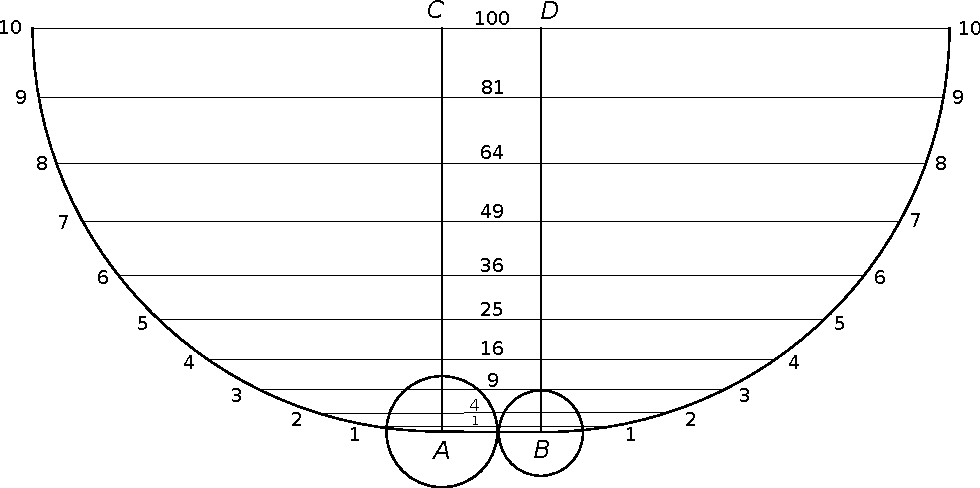
\includegraphics[width=0.98\textwidth]{gesamttex/edit_VIII,3/images/LH_35_09_23_015-020_d.pdf}}%
  \vspace*{0.5em}
  \centerline{\lbrack\textit{Fig.~1}\rbrack}%
  \label{LH_35_09_23_017v_Fig.1}%
  \vspace{1.5em}%
%  \newpage%
%
\pstart%
\noindent%
\edtext{}{%
{\xxref{LH_35_09_23_017v_Regnault-Versuche-1}{LH_35_09_23_018r_Regnault-Versuche-2}}%
{\lemma{Corpora \lbrack...\rbrack\ designatorum}%
\Cfootnote{%
Siehe zu den hier beschriebenen Versuchsbedingungen:
%\protect\index{Namensregister}{\textso{Regnauld} (Regnaud; Regnaldus), Fran\c{c}ois de 1626\textendash1689}%
%\textsc{Regnauld}, \cite{02021}Brief an Monconys vom 21.\ Dezember 1655,
% in: \protect\index{Namensregister}{\textso{Monconys} (Monconisius), Balthasar de 1611\textendash1665}\textsc{B.~de Monconys,} \cite{00118}\title{Journal des voyages}, Teil III: \glqq Lettres escrittes à Monsieur de Monconys\grqq\ (Lyon 1666, S.~52\textendash56, getrennte Paginierung).
a.a.O. (S.~52\,f.).\cite{02021}\cite{00118}
%Das Diagramm \lbrack\textit{Fig.~1}\rbrack\ stammt ebendorther (Fig.~8), wobei Leibniz die Punkte \textit{A} bis \textit{D} anders bezeichnet hat als Regnauld.\protect\index{Namensregister}{\textso{Regnauld} (Regnaud; Regnaldus), Fran\c{c}ois de 1626\textendash1689}
}}}%
%
Corpora duo%
\edlabel{LH_35_09_23_017v_Regnault-Versuche-1}%
\edlabel{LH_35_09_23_018v_iiiSchichtKomm-1}
%
\edtext{\textit{A}, \textit{B},}{%
\lemma{\textit{A}, \textit{B},}\Bfootnote{%
\textit{erg.~L}}}
%
incurrens%
\protect\index{Sachverzeichnis}{corpus incurrens}
et excipiens%
\protect\index{Sachverzeichnis}{corpus excipiens}%
\lbrack,\rbrack\
pendula%
\protect\index{Sachverzeichnis}{corpus pendulum}%
\protect\index{Sachverzeichnis}{pendulum}
intelliguntur ex iisdem semidiametris
%
\edtext{\textit{CA}, \textit{CB},}{%
\lemma{\textit{CA}, \textit{CB},}\Bfootnote{%
\textit{erg.~L}}}
%
ita ut in perpendiculari quiescentia se tangant:
et circuli quos vibrando describerent sint in eodem plano,
et centra suspensionis%
\protect\index{Sachverzeichnis}{centrum suspensionis}
%
\edtext{\textit{CD}}{%
\lemma{\textit{CD}}\Bfootnote{%
\textit{erg.~L}}}
%
in eadem horizontali;
non minus ac centra gravitatis%
\protect\index{Sachverzeichnis}{centrum gravitatis}
et magnitudinis corporum%
\protect\index{Sachverzeichnis}{magnitudo corporum concurrentium}
\textit{A}, \textit{B}.
\pend%
%
\pstart%
% \noindent%
%\edtext{}{%
%\lemma{\hspace*{1,6mm}%
%\lbrack\textit{Fig.~1}\rbrack%
%}\killnumber%
%\Cfootnote{%
%Das Diagramm stammt aus Regnauld (Fig.~8), wobei Leibniz die Punkte \textit{A} bis \textit{D} anders bezeichnet als Regnauld. \protect\index{Namensregister}{\textso{Regnauld} (Regnaud; Regnaldus), Fran\c{c}ois de 1626\textendash1689}\textsc{F.~Regnauld}, \cite{02021}Brief an B.~de Monconys vom 21.\ Dezember 1655, in: \protect\index{Namensregister}{\textso{Monconys} (Monconisius), Balthasar de 1611\textendash1665}\textsc{B.~de Monconys,} \cite{00118}\title{Journal des voyages}, Teil III: \glqq Lettres escrittes à Monsieur de Monconys\grqq\ (Lyon 1666, S.~52\textendash56, getrennte Paginierung).%
%}}%
Filum \textit{AC} vel \textit{BD}%
\protect\index{Sachverzeichnis}{filum}
divisum in 100 partes
et notatum numeris quadratis 100. 81. 64 etc.%
\protect\index{Sachverzeichnis}{numerus quadratus}
usque ad 1 descendendo.
Lineae horizonti parallelae per
%
\edtext{\lbrack puncta\rbrack}{%
\lemma{lineas}\Bfootnote{%
\textit{L~ändert Hrsg.}}}
%
divisionis ductae
%
\edtext{secabunt quadrantes \textit{CA}10, \textit{DB}10%
\protect\index{Sachverzeichnis}{quadrans}
centris \textit{C} et \textit{D} descriptos,}{%
\lemma{secabunt}\Bfootnote{%
\textit{(1)}~circulos in punctis intersection
\textit{(2)}~quadrantes \textit{CA}10, % \textit{DB} 10 centris \textit{C} et 
\lbrack...\rbrack\ \textit{D} descriptos,%
~\textit{L}}}
%
et punctis sectionis \makebox[1.0\textwidth][s]{ascribuntur
radices numerorum quadratorum,%
\protect\index{Sachverzeichnis}{radix numeri quadrati}
scilicet 10. 9. 8 etc. usque ad 1.
Constat}%
\pend
\newpage
\pstart
\noindent
%
ex \edtext{traditis Galilaei}{% e dimostrazioni matematiche
\lemma{traditis Galilaei}\Cfootnote{%
Siehe G.~\textsc{Galilei}, \textit{Discorsi}, giornata III, theorema II, prop. II
(Leiden 1638, S.~171\,f.;\cite{00050}
% Bologna 1656\cite{00260}, S.~130\,f.; 
\textit{GO} VIII, S.~209\,f.).\cite{00048}
Hierauf verweist auch \textsc{Regnauld}, \cite{02021}Brief an Monconys vom 21.\ Dezember 1655 (S.~52).%
\cite{02021}\cite{00118}%
\protect\index{Namensregister}{\textso{Regnauld} (Regnaud; Regnaldus), Fran\c{c}ois de 1626\textendash1689}%
}}
%
corporum ex%
\protect\index{Sachverzeichnis}{corpus descendens}
%
\edtext{punctis}{%
\lemma{punctis}\Bfootnote{%
\textit{erg.~L}}}
%
100. 81. 64 etc.
descendentium celeritates%
\protect\index{Sachverzeichnis}{celeritas descensus}
esse ut 10. 9. 8 etc.
et eandem acquiri celeritatem%
\protect\index{Sachverzeichnis}{celeritas descensus}
si ex punctis 10. 9. 8 descendant,
ac si ex punctis 100. 81. 64 etc. descenderent.
Ergo corpora ex punctis 10. 9. 8. etc. descendentia%
\protect\index{Sachverzeichnis}{corpus descendens}
acquirunt celeritates%
\protect\index{Sachverzeichnis}{celeritas descensus}
ut 10. 9. 8 etc.
Rursus corpora%
\protect\index{Sachverzeichnis}{corpus ascendens}
habentia celeritatem%
\protect\index{Sachverzeichnis}{celeritas ascensus}
ut 8 ascendunt usque ad 8 etc.
(abstrahendo ab aeris resistentia).%
\protect\index{Sachverzeichnis}{resistentia aeris}%
\protect\index{Sachverzeichnis}{aer resistens}
Ergo possumus celeritates in statu perpendiculari quaesitas%
\protect\index{Sachverzeichnis}{celeritas in statu perpendiculari quaesita}
%
\lbrack18~r\textsuperscript{o}\rbrack\ %    %    %    %    Blatt 18r
%
ante concursum%
\protect\index{Sachverzeichnis}{celeritas ante concursum}%
\protect\index{Sachverzeichnis}{concursus corporum}
mensurare descensu:%
\protect\index{Sachverzeichnis}{descensus corporis}%
\protect\index{Sachverzeichnis}{descensus penduli}
residuas post ictum%
\protect\index{Sachverzeichnis}{celeritas residua post ictum}%
\protect\index{Sachverzeichnis}{ictus}
mensurabimus
%
\edtext{incurrentis}{%
\lemma{incurrentis}\Bfootnote{%
\textit{erg.~L}}}
%
continuatione%
\protect\index{Sachverzeichnis}{continuatio corporis incurrentis}
vel reflexione,%
\protect\index{Sachverzeichnis}{reflexio corporis incurrentis}
communicatas quiescenti%
\protect\index{Sachverzeichnis}{celeritas communicata quiescenti}%
\protect\index{Sachverzeichnis}{celeritas communicata post ictum}
mensurabimus
ipsius ascensu;%
\protect\index{Sachverzeichnis}{ascensus corporis excipientis}
ad aliquod punctorum in circulo designatorum.%
\protect\index{Sachverzeichnis}{circulus}%
\edlabel{LH_35_09_23_018r_Regnault-Versuche-2}
\pend%
%
\pstart%
\edtext{Quando descensus satis altus%
\protect\index{Sachverzeichnis}{descensus penduli}%
\protect\index{Sachverzeichnis}{descensus corporis incurrentis}
seu ictus satis fortis,%
\protect\index{Sachverzeichnis}{ictus satis fortis}
id est quando descensus%
\protect\index{Sachverzeichnis}{descensus penduli}%
\protect\index{Sachverzeichnis}{descensus corporis incurrentis}
ex 3 et ultra 3,
tunc semper continuatio%
\protect\index{Sachverzeichnis}{continuatio penduli}%
\protect\index{Sachverzeichnis}{continuatio corporis incurrentis}
experimenti%
\protect\index{Sachverzeichnis}{experimentum}
major continuatione%
\protect\index{Sachverzeichnis}{continuatio penduli}%
\protect\index{Sachverzeichnis}{continuatio corporis incurrentis}
calculi,%
\protect\index{Sachverzeichnis}{calculus}
et tanto magis,
quando corpora magis accedunt ad aequalitatem%
\protect\index{Sachverzeichnis}{aequalitas corporum concurrentium}
%
\edtext{}{%
{\xxref{LH_35_09_23_018r_MargNB-1}{LH_35_09_23_018r_MargNB-2}}%
{\lemma{\textit{Am Rand, auf das Satzglied in eckigen Klammern bezogen:}}\Afootnote{NB}}}%
%
\edlabel{LH_35_09_23_018r_MargNB-1}%
\edtext{\lbrack excepto}{%
\lemma{\lbrack excepto}\Cfootnote{%
Eckige Klammer von Leibniz.}}
uno casu,%
\protect\index{Sachverzeichnis}{casus}
4 in 1 ex 7,
ubi error forte in%
\protect\index{Sachverzeichnis}{error in experimento}
\edtext{experimento\rbrack.}{%
\lemma{experimento\rbrack}\Cfootnote{%
Eckige Klammer von Leibniz.}}%
\edlabel{LH_35_09_23_018r_MargNB-2}
%
Ratio%
\protect\index{Sachverzeichnis}{ratio}%
\lbrack:\rbrack\
quia quo major ictus,
eo magis vires exerit percussio.%
\protect\index{Sachverzeichnis}{vis exerta percussione}%
\protect\index{Sachverzeichnis}{percussio}
At lignum%
\protect\index{Sachverzeichnis}{lignum}
non eam omnino percipit
ut chalybs,%
\protect\index{Sachverzeichnis}{chalybs}
et ita medium tenet
inter corpus molle%
\protect\index{Sachverzeichnis}{corpus molle}
et durum.%
\protect\index{Sachverzeichnis}{corpus durum}
In molli%
\protect\index{Sachverzeichnis}{corpus molle}
autem major continuatio,%
\protect\index{Sachverzeichnis}{continuatio corporis incurrentis}%
\protect\index{Sachverzeichnis}{continuatio penduli}
minor ascensus%
\protect\index{Sachverzeichnis}{ascensus corporis excipientis}%
\protect\index{Sachverzeichnis}{ascensus penduli}
quam in duro,%
\protect\index{Sachverzeichnis}{corpus durum}
ergo et in his experimentis%
\protect\index{Sachverzeichnis}{experimentum}
quae in corporibus nonnihil mollibus%
\protect\index{Sachverzeichnis}{corpus molle}
facta,
major continuatio,%
\protect\index{Sachverzeichnis}{continuatio corporis incurrentis}%
\protect\index{Sachverzeichnis}{continuatio penduli}
minor ascensus%
\protect\index{Sachverzeichnis}{ascensus corporis excipientis}%
\protect\index{Sachverzeichnis}{ascensus penduli}
quam in calculo%
\protect\index{Sachverzeichnis}{calculus}
secundum dura%
\protect\index{Sachverzeichnis}{corpus durum}
facto.%
}{%
\lemma{Quando}\Bfootnote{%
\hspace{-0,5mm}descensus % satis altus seu ictus 
\lbrack...\rbrack\ satis fortis
\textbar~id est % quando descensus ex 3 et 
\lbrack...\rbrack\ ultra 3 \textit{erg.}~%
\textbar\ tunc semper % ....
\lbrack...\rbrack\ ergo et in
\textit{(1)}~hoc experimento quod
\textit{(2)}~his experimentis % quae in corporibus nonnihil 
\lbrack...\rbrack\ mollibus facta,
\textit{(a)}~minor
\textit{(b)}~major continuatio,
\lbrack...\rbrack\ dura facto.
\textit{erg.~L}}}
%
\lbrack18~v\textsuperscript{o}\rbrack\ %    %    %    %    Blatt 18v
%
\pend%
%
\pstart%
% \noindent%
Si continuatio%
\protect\index{Sachverzeichnis}{continuatio corporis incurrentis}%
\protect\index{Sachverzeichnis}{continuatio penduli}
experimenti%
\protect\index{Sachverzeichnis}{experimentum}
%
\edtext{parum differt a continuatione}{%
\lemma{parum}\Bfootnote{%
\textit{(1)}~excedit continuationem
\textit{(2)}~differt a continuatione%
~\textit{L}}}
%
calculi,%
\protect\index{Sachverzeichnis}{calculus}
ascensus tamen experimenti
%
\edtext{multum differre debet
ab ascensu%
\protect\index{Sachverzeichnis}{ascensus corporis excipientis}%
\protect\index{Sachverzeichnis}{ascensus penduli}
calculi,%
\protect\index{Sachverzeichnis}{calculus}
et eo magis
quo major corporum differentia,%
\protect\index{Sachverzeichnis}{differentia corporum concurrentium}
quia continuans incurrens%
\protect\index{Sachverzeichnis}{corpus incurrens continuans}
majus ponitur excipiente ascendente.%
\protect\index{Sachverzeichnis}{corpus excipiens ascendens}
Et illius celeritas,%
\protect\index{Sachverzeichnis}{celeritas continuationis}
continuatio nempe%
\protect\index{Sachverzeichnis}{continuatio corporis incurrentis}%
\protect\index{Sachverzeichnis}{continuatio penduli}
% \lbrack,\rbrack\
huic minori ademta,
multam ei adimit celeritatem.%
\protect\index{Sachverzeichnis}{celeritas ademta}%
}{%
\lemma{multum}\Bfootnote{%
\textit{(1)}~ab eo
\textit{(2)}~differre debet ab ascensu calculi,
\textbar~et eo % magis quo major 
\lbrack...\rbrack\ corporum differentia,~\textit{erg.}~%
\textbar\ quia
\textit{(a)}~vis
\textit{(b)}~continuans incurrens % majus ponitur excipiente 
\lbrack...\rbrack\ ascendente. Et
\textit{(aa)}~vis illius exigua
\textit{(bb)}~illius celeritas, continuatio nempe; multam ei adimit celeritatem.%
~\textit{L}}}
%
\pend%
\newpage
\pstart%
Aliqua semper vis%
\protect\index{Sachverzeichnis}{vis perdita}
in experimento%
\protect\index{Sachverzeichnis}{experimentum}
perdita reperietur,
nunquam certe augebitur quantitas motus.%
\protect\index{Sachverzeichnis}{quantitas motus}
%
His ergo experimentis%
\protect\index{Sachverzeichnis}{experimentum}
systemata
%
\edtext{Hugenii,%
\protect\index{Namensregister}{\textso{Huygens} (Hugenius, Ugenius, Hugens, Huguens), Christiaan 1629-1695}%
\protect\index{Sachverzeichnis}{systema Hugenii}%
}{%
\lemma{Hugenii}%
\Cfootnote{%
Vgl. C.~\textsc{Huygens}, \cite{00529}\glqq Regles du mouvement dans la rencontre des corps\grqq, \cite{00157}\textit{JS} 18.~März 1669 (Pariser Ausgabe, S.~22\textendash24; \textit{HO} XVI, S.~179\textendash181).%
}}
%
\edtext{Wrenni,%
\protect\index{Namensregister}{\textso{Wren} (Wrennus), Christopher 1632-1723}%
\protect\index{Sachverzeichnis}{systema Wrenni}%
}{%
\lemma{Wrenni}%
\Cfootnote{%
Vgl. C.~\textsc{Wren}, \cite{01066}\glqq Theory concerning the same subject\grqq, \cite{00158}\textit{PT} III (1668/1669), S.~867\,f.%
}}
%
\edtext{Wallisii%
\protect\index{Namensregister}{\textso{Wallis} (Wallisius), John 1616-1703}%
\protect\index{Sachverzeichnis}{systema Wallisii}%
}{%
\lemma{Wallisii}%
\Cfootnote{%
Vgl. J.~\textsc{Wallis}, \cite{01065}\glqq A summary account \lbrack...\rbrack\ of the general laws of motion\grqq, \cite{00158}\textit{PT} III (1668/1669), S.~864\textendash866;
%
\textsc{Ders.}, \cite{00301}\textit{Mechanica}, pars~III, cap.~11 u.~13 (Bd.~II, London 1671, S.~660\textendash682, 686\textendash707; \cite{01008}\textit{WO} I, S.~1002\textendash1015, 1018\textendash1031).%
}}
%
et
%
\edtext{Mariotti%
\protect\index{Namensregister}{\textso{Mariotte}, Edme, Seigneur de Chazeuil ca. 1620-1684}%
\protect\index{Sachverzeichnis}{systema Mariotti}%
}{%
\lemma{Mariotti}%
\Cfootnote{%
Vgl. E.~\textsc{Mariotte}, \cite{00311}\textit{De la percussion}, Paris 1673.%
}}
%
evertuntur.%
\edlabel{LH_35_09_23_018v_iiiSchichtKomm-2}
%
\pend%
 %\newpage%
\vspace{1.0em}%
%
\pstart%
\noindent%
\lbrack\textit{Nachträglich (\glqq post reformationem\grqq) hinzugefügt}:\rbrack%
\edtext{}{\lemma{\textit{\glqq post reformationem\grqq}}\Cfootnote{%
Siehe zur Textgenese von N.~\ref{dcc_06-2} %??S01\textsubscript{8} 
die editorische Vorbemerkung, S.~\refpassage{dcc_intro_VI-II_fzr-1}{dcc_intro_VI-II_fzr-2}.%
}}
\pend%
\vspace{0.5em}%
%
\pstart%
\noindent%
Video%
\edlabel{LH_35_09_23_018v_ivSchicht-1}
jam in quo sit hoc loco\textls{ erratum.}
Nempe%
\protect\index{Sachverzeichnis}{erratum de aestimatione virium}
vis in corpore%
\protect\index{Sachverzeichnis}{vis in corpore}
non aestimanda est a celeritate et magnitudine corporis;%
\protect\index{Sachverzeichnis}{vis aestimanda a celeritate}
sed ab altitudine ex qua decidit.%
\protect\index{Sachverzeichnis}{vis aestimanda ab altitudine}
Sunt autem altitudines ex quibus corpora deciderunt,%
\protect\index{Sachverzeichnis}{altitudo ut quadratum celeritatis}
ut quadrata quaesitarum celeritatum.%
\protect\index{Sachverzeichnis}{celeritas quaesita}%
\protect\index{Sachverzeichnis}{quadratum celeritatis}
Ergo et vires,%
\protect\index{Sachverzeichnis}{vis in duplicata ratione celeritatis}
corporibus positis iisdem.
Generaliter autem vires sunt in composita ratione
ex simplici corporum et duplicata celeritatum.%
\protect\index{Sachverzeichnis}{vis in duplicata ratione celeritatis}
Hinc duo corpora aequalium sunt virium,%
\protect\index{Sachverzeichnis}{corpora virium aequalium}
non
%
\edtext{ut vulgo putant,}{%
\lemma{ut vulgo putant}\Cfootnote{%
Siehe etwa
\protect\index{Namensregister}{\textso{Wallis} (Wallisius), John 1616-1703}%
\textsc{Wallis}, \cite{00301}\textit{Mechanica}, pars~III, cap.~11, prop.~4; cap.~13, prop.~3 (Bd.~II, S.~665; 695; \cite{01008}\textit{WO} I, S.~1005; 1023);
vor allem
\protect\index{Namensregister}{\textso{Mariotte}, Edme, Seigneur de Chazeuil ca. 1620-1684}%
\textsc{Mariotte}, \cite{00311}\textit{De la percussion}, partie I, prop. 6, avertissement (S.~40\textendash44, bes. S.~42).
Leibniz hatte diese Stellen in Paris exzerpiert:
Vgl. \textit{LSB} VIII,~2 N.~8, S.~83.1\textendash2; 89.19\textendash22;\cite{01343}
N.~50, S.~425.10\textendash12.\cite{01292}%
}}
%
\edtext{cum celeritates sunt}{%
\lemma{cum}\Bfootnote{%
\textit{(1)}~momenta sunt
\textit{(2)}~celeritates sunt%
~\textit{L}}}
%
ut corpora reciproce,
sed cum quadrata celeritatum%
\protect\index{Sachverzeichnis}{quadratum celeritatis}
sunt ut corpora
%
\edtext{reciproce.
Hinc patet}{%
\lemma{reciproce.}\Bfootnote{%
\textit{(1)}~Hinc id quod
\textit{(2)}~Hinc patet%
~\textit{L}}}
%
non eandem servari quantitatem motus,%
\protect\index{Sachverzeichnis}{quantitas motus non servata}
sed tantum eandem vim.%
\protect\index{Sachverzeichnis}{vis servata eadem}
\pend%
%
\pstart%
Porro ipsa quadrata celeritatum%
\protect\index{Sachverzeichnis}{quadratum celeritatis}
vocabimus momenta,%
\protect\index{Sachverzeichnis}{momentum ut quadratum celeritatis}
ita ut sint momenta%
\protect\index{Sachverzeichnis}{momentum ut quadratum celeritatis}
ad vim,
uti celeritas%
\protect\index{Sachverzeichnis}{celeritas quaesita}
ad quantitatem motus.
%\pend%
%%
%\pstart%
In nostro systemate%
\protect\index{Sachverzeichnis}{systema nostrum}
necesse
%
\edtext{est momenta%
\protect\index{Sachverzeichnis}{momentum ut quadratum celeritatis}
esse}{%
\lemma{est}\Bfootnote{%
\textit{(1)}~celeritates esse
\textit{(2)}~momenta esse%
~\textit{L}}}
%
quadrata celeritatum;%
\protect\index{Sachverzeichnis}{quadratum celeritatis}
quia effectus%
\protect\index{Sachverzeichnis}{effectus}
est ascensus%
\protect\index{Sachverzeichnis}{ascensus corporis excipientis}%
\protect\index{Sachverzeichnis}{ascensus penduli}%
\protect\index{Sachverzeichnis}{ascensus ut effectus}
ad quem corpus ascendendo pervenire potest;%
\protect\index{Sachverzeichnis}{corpus excipiens}
ascensus autem sunt ut quadrata celeritatum.%
\protect\index{Sachverzeichnis}{ascensus ut quadratum celeritatis}
%\pend%
%%
%\pstart%
In alio forte systemate Mundi,%
\protect\index{Sachverzeichnis}{systema mundi alium}
ubi celeritates aliam habent relationem ad altitudines,%
\protect\index{Sachverzeichnis}{relatio celeritatis ad altitudinem}
etiam alia facienda esset virium aestimatio.%
\protect\index{Sachverzeichnis}{aestimatio virium}
\pend%
%
\pstart%
Porro%
\edlabel{LH_35_09_23_018v_occasionalismus_jyr-1}
ex his sequitur
corpora non a se ipsis ferri,%
\protect\index{Sachverzeichnis}{corpus latum a se}%
\protect\index{Sachverzeichnis}{corpus latum impetu conceptu}
impetu concepto,%
\protect\index{Sachverzeichnis}{impetus conceptus}
\lbrack\textendash\rbrack\
quomodo enim meminisse possunt
ex qua altitudine deciderint,
aut quomodo intelligere
in quo systemate ferantur,%
\protect\index{Sachverzeichnis}{systema mundi alium}
\lbrack\textendash\rbrack\
sed necesse est vel
ea perpetuo ferri a motore generali%
\protect\index{Sachverzeichnis}{motor generalis}
(\protect\vphantom)%
quod tamen non satisfacit,
%
\edtext{quia propriam vim etiam corpus haberet,%
\protect\index{Sachverzeichnis}{vis corporis propria}}{%
\lemma{quia}\Bfootnote{%
\textit{(1)}~fieret
\textit{(2)}~propriam
\textbar~tamen \textit{streicht Hrsg.}~%
\textbar\ vim corpus haberet,%
~\textit{L}}}
%
quae cum generali%
\protect\index{Sachverzeichnis}{vis generalis}
componeretur%
\protect\vphantom()
vel potius continuo%
\protect\index{Sachverzeichnis}{corpus continuo impulsum}
%
\edtext{impelli a sapientissima causa,%
\protect\index{Sachverzeichnis}{causa sapientissima}%
}{%
\lemma{impelli}\Bfootnote{%
\textit{(1)}~ab intelligen
\textit{(2)}~a sapientissima causa,%
~\textit{L}}}
%
quae omnium meminit fallique non potest,
adeoque nihil aliud esse Leges motus% ,%
\protect\index{Sachverzeichnis}{lex motus}
quam rationes divinae voluntatis,%
\protect\index{Sachverzeichnis}{ratio voluntatis divinae}
%
\edtext{\lbrack quae\rbrack}{%
\lemma{qui}\Bfootnote{%
\textit{L~ändert Hrsg.}}}
%
effectus
%
\edtext{causis assimilat,%
\protect\index{Sachverzeichnis}{assimilatio effectus causae}%
\protect\index{Sachverzeichnis}{effectus causae assimilatus}%
\protect\index{Sachverzeichnis}{causa effectui assimilata}}{%
\lemma{causis}\Bfootnote{%
\textit{(1)}~assimilent,
\textit{(2)}~assimilat,%
~\textit{L}}}
%
quantum patitur ratio rerum.%
\protect\index{Sachverzeichnis}{ratio rerum}%
\edlabel{LH_35_09_23_018v_occasionalismus_jyr-2}
\pend%
%
\pstart%
Corrigi%
\edlabel{LH_35_09_23_018v_subfinem-1}
potest Tabula praecedens,%
\protect\index{Sachverzeichnis}{tabula}
pro descensu%
\protect\index{Sachverzeichnis}{descensus corporis incurrentis}%
\protect\index{Sachverzeichnis}{descensus penduli}
1. 2. 3. 4. 5 etc.
scribendo 1. 4. 9. 16. 25 etc.
adeoque primum calculum continuationis%
\protect\index{Sachverzeichnis}{calculus continuationis}%
\protect\index{Sachverzeichnis}{continuatio corporis incurrentis}%
\protect\index{Sachverzeichnis}{continuatio penduli}
vel ascensus,%
\protect\index{Sachverzeichnis}{calculus ascensus}%
\protect\index{Sachverzeichnis}{ascensus corporis excipientis}%
\protect\index{Sachverzeichnis}{ascensus penduli}
nempe 16 in 1,
8 in 1,
et 4 in 1,
et 2 in 1,
et 1 in 1,
non multiplicando per 2. 3. 4. 5
sed per 4. 9. 16. 25
ad producendos calculos reliquos;
denique experimenta ducendo in re ipsa.
\pend%
%
\pstart%
Et hoc factum in Tabula sequente.%
\protect\index{Sachverzeichnis}{tabula}%
\edlabel{LH_35_09_23_018v_subfinem-2}%
\edlabel{LH_35_09_23_018v_ivSchicht-2}
\pend%
\vspace{1.0em}%
%
\pstart%
\noindent%
\hspace{108mm}%
Tabula III%
\protect\index{Sachverzeichnis}{tabula}
%
\lbrack19~r\textsuperscript{o}\rbrack
%
\edtext{}{%
\lemma{\hspace{1,6mm}\textit{Zur tabellarischen Darstellung auf S.~\pageref{LH_35_09_23_019r_tab3}}}%
\killnumber\Cfootnote{%
Die zur Reihe \textit{4 descens.} und Spalte \textit{16~in~1} gehörige Zelle gab irrtümlich den experimentellen Wert 9~plus an.
Der richtige Wert 9 lässt sich anhand der tabellarischen Darstellung auf S.~\pageref{LH_35_09_23_018r_tab2} bestimmen.
\quad
Die zur Reihe \textit{25~descens.} und Spalte \textit{16~in~1} gehörige Zelle gab irrtümlich den theoretischen Wert $\displaystyle57 + \frac{27}{289}$ an.
Der richtige Wert $\displaystyle57 + \frac{127}{289}$ lässt sich anhand der tabellarischen Darstellung auf S.~\pageref{LH_35_09_23_018r_tab2} bestimmen.
\quad
Die zur Reihe \textit{64~descens.} und Spalte \textit{16~in~1} gehörige Zelle gab irrtümlich den theoretischen Wert $\displaystyle56 + \frac{112}{578}$ an.
Der richtige Wert $\displaystyle54 + \frac{468}{578}$ lässt sich anhand der tabellarischen Darstellung auf S.~\pageref{LH_35_09_23_018r_tab2} bestimmen.
\quad
Die zur Reihe \textit{64~descens.} und Spalte \textit{4~in~1} gehörige Zelle gab irrtümlich den theoretischen Wert $\displaystyle34 + \frac{8}{50}$ an.
Der richtige Wert $\displaystyle34 + \frac{28}{50}$ lässt sich anhand der tabellarischen Darstellung auf S.~\pageref{LH_35_09_23_018r_tab2} bestimmen.
\quad
}}
\pend%
\newpage%
% \vspace{1.5em}%
%
\pstart%
\noindent%
%
\lbrack\textit{In der folgenden Tabelle ist der in serifenloser Schrift gesetzte Text von Schreiberhand}:\rbrack\
\pend%
\vspace{0.5em}%
%
\pstart%
\noindent%
%
% \rotatebox{90}{
%%
%\lbrack19~r\textsuperscript{o}\rbrack
%%
% }
%    %    %    %    Blatt 19r
\label{LH_35_09_23_019r_tab3}%
%
\protect\index{Sachverzeichnis}{descensus penduli}%
\protect\index{Sachverzeichnis}{velocitas descensus}%
\protect\index{Sachverzeichnis}{celeritas descensus}%
\protect\index{Sachverzeichnis}{ascensus penduli}%
\protect\index{Sachverzeichnis}{velocitas ascensus}%
\protect\index{Sachverzeichnis}{celeritas ascensus}%
\protect\index{Sachverzeichnis}{continuatio penduli}%
\protect\index{Sachverzeichnis}{vis perdita}%
\protect\index{Sachverzeichnis}{velocitas continuationis}%
\protect\index{Sachverzeichnis}{celeritas continuationis}%
\protect\index{Sachverzeichnis}{calculus}%
\protect\index{Sachverzeichnis}{experimentum}%
\pend%
%\vspace{0.5em}%
%
\pstart%
\noindent%
\resizebox{\textwidth}{!}{%
% \rotatebox{90}{%
\begin{tabular}{r|lr|lr|lr|lr|lr}
&
\multicolumn{2}{c|}{16 in 1}
&
\multicolumn{2}{c|}{8 in 1}
&
\multicolumn{2}{c|}{4 in 1}
&
\multicolumn{2}{c|}{2 in 1}
&
\multicolumn{2}{c}{1 in 1}
\\
& Contin.
& Ascensus
%
& Contin.
& Ascens.
%
& Contin.
& Asc.
%
& Contin.
& Asc.
%
& Contin.
& Asc.
%
\\
\hline
%
% % % %  descensus 1
%
\rule[0mm]{0mm}{4mm}%
\textsf{1 descens.}
& & & & & & & & & & 
\\
\textsf{Calculus}
& 
\textsf{$\displaystyle\frac{\textsf{495}}{\textsf{578}}$}
& 
\textsf{$\textsf{2 + }\displaystyle\frac{\textsf{86}}{\textsf{289}}$}
& 
\textsf{$\displaystyle\frac{\textsf{119}}{\textsf{162}}$}
& 
\textsf{$\textsf{2 + }\displaystyle\frac{\textsf{10}}{\textsf{81}}$}
& 
\textsf{$\displaystyle\frac{\textsf{27}}{\textsf{50}}$}
& 
\textsf{$\textsf{1 + }\displaystyle\frac{\textsf{21}}{\textsf{25}}$}
& 
\textsf{$\displaystyle\frac{\textsf{5}}{\textsf{18}}$}
& 
\textsf{$\textsf{1 + }\displaystyle\frac{\textsf{4}}{\textsf{9}}$}
& 
\textsf{$\displaystyle\frac{\textsf{0}}{\textsf{8}}$}
& 
\textsf{1}
\\
& & & & & & & & & & 
\\
\textsf{Experimenta}
& 
\textsf{$ \displaystyle\frac{\textsf{9}}{\textsf{16}} $} fere
& 
\textsf{$ \textsf{2 + }\displaystyle\frac{\textsf{1}}{\textsf{4}} $}
& 
\textsf{0}
& 
\textsf{$ \textsf{2 + }\displaystyle\frac{\textsf{1}}{\textsf{4}} $}
& 
\textsf{0}
& 
\textsf{$ \textsf{2 + }\displaystyle\frac{\textsf{1}}{\textsf{4}}$}
& 
& 
& 
& 
\\
& (NB) & & & NB & & NB & & & & 
\\
\hline
%
% % % %  descensus 4
%
\rule[0mm]{0mm}{4mm}%
\textsf{4 descens.}
& & & & & & & & & & 
\\
\textsf{Calculus}
& 
\textsf{$ \textsf{3 + }\displaystyle\frac{\textsf{246}}{\textsf{578}} $}
& 
\textsf{$ \textsf{9 + }\displaystyle\frac{\textsf{55}}{\textsf{289}} $}
& 
\textsf{$ \textsf{2 + }\displaystyle\frac{\textsf{152}}{\textsf{162}} $}
& 
\textsf{$ \textsf{8 + }\displaystyle\frac{\textsf{40}}{\textsf{81}} $}
& 
\textsf{$ \textsf{2 + }\displaystyle\frac{\textsf{8}}{\textsf{50}} $}
& 
\textsf{$ \textsf{7 + }\displaystyle\frac{\textsf{9}}{\textsf{25}} $}
& 
\textsf{$ \textsf{1 + }\displaystyle\frac{\textsf{2}}{\textsf{18}} $}
& 
\textsf{$ \textsf{5 + }\displaystyle\frac{\textsf{7}}{\textsf{9}} $}
& 
\textsf{$ \displaystyle\frac{\textsf{0}}{\textsf{8}} $}
& 
\textsf{4}
\\
& & & & & & & & & & 
\\
\textsf{Experimenta}
& 
\textsf{$ \textsf{2 + }\displaystyle\frac{\textsf{1}}{\textsf{4}} $ plus}
& 
\textsf{[9]} %% \textsf{9 plus} %%
& 
\textsf{$ \textsf{2 + }\displaystyle\frac{\textsf{1}}{\textsf{4}} $ plus}
& 
\textsf{9 plus}
& 
\textsf{1}
& 
\textsf{$ \textsf{6 + }\displaystyle\frac{\textsf{19}}{\textsf{25}} $}
& 
& 
& 
\textsf{0 plus}
& 
\textsf{$ \textsf{3 + }\displaystyle\frac{\textsf{1}}{\textsf{16}} $}
\\
& & & & NB & & NB & & & (NB) &
\\
\hline
%
% % % %  descensus 9
%
\rule[0mm]{0mm}{4mm}%
\textsf{9 descens.}
& & & & & & & & & & 
\\
\textsf{Calculus}
& 
\textsf{$ \textsf{7 + }\displaystyle\frac{\textsf{409}}{\textsf{578}} $}
& 
\textsf{$ \textsf{20 + }\displaystyle\frac{\textsf{196}}{\textsf{289}} $}
& 
\textsf{$ \textsf{6 + }\displaystyle\frac{\textsf{99}}{\textsf{162}} $}
& 
\textsf{$ \textsf{19 + }\displaystyle\frac{\textsf{9}}{\textsf{81}} $}
& 
\textsf{$ \textsf{4 + }\displaystyle\frac{\textsf{43}}{\textsf{50}} $}
& 
\textsf{$ \textsf{16 + }\displaystyle\frac{\textsf{14}}{\textsf{25}} $}
& 
\textsf{$ \textsf{2 + }\displaystyle\frac{\textsf{9}}{\textsf{18}} $}
& 
\textsf{$ \textsf{13 + }\displaystyle\frac{\phantom{m}}{\phantom{m}} $}
& 
\textsf{$ \displaystyle\frac{\textsf{0}}{\textsf{8}} $}
& 
\textsf{9}
\\
& & & & & & & & & & 
\\
\textsf{Experimenta}
& 
\textsf{$ \textsf{6 + }\displaystyle\frac{\textsf{1}}{\textsf{4}} $}
& 
\textsf{$ \textsf{17 + }\displaystyle\frac{\textsf{16}}{\textsf{25}} $}
& 
\textsf{$ \textsf{5 + }\displaystyle\frac{\textsf{1}}{\textsf{16}} $}
& 
\textsf{25 minus}
& 
\textsf{4 minus}
& 
\textsf{16}
& 
& 
& 
& 
\\
& & & & NB & & & & & & 
\\
\hline
%
% % % %  descensus 16
%
\rule[0mm]{0mm}{4mm}%
\textsf{16 descens.}
& & & & & & & & & &
\\
\textsf{Calculus}
& 
\textsf{$ \textsf{13 + }\displaystyle\frac{\textsf{406}}{\textsf{578}} $}
& 
\textsf{$ \textsf{36 + }\displaystyle\frac{\textsf{220}}{\textsf{289}} $}
& 
\textsf{$ \textsf{11 + }\displaystyle\frac{\textsf{122}}{\textsf{162}} $}
& 
\textsf{$ \textsf{33 + }\displaystyle\frac{\textsf{79}}{\textsf{81}} $}
& 
\textsf{$ \textsf{8 + }\displaystyle\frac{\textsf{32}}{\textsf{50}} $}
& 
\textsf{$ \textsf{29 + }\displaystyle\frac{\textsf{11}}{\textsf{25}} $}
& 
\textsf{$ \textsf{4 + }\displaystyle\frac{\textsf{8}}{\textsf{18}} $}
& 
\textsf{$ \textsf{23 + }\displaystyle\frac{\textsf{1}}{\textsf{9}} $}
& 
\textsf{$ \displaystyle\frac{\textsf{0}}{\textsf{8}} $}
& 
\textsf{16}
\\
& & & & & & & & & & 
\\
\textsf{Experimenta}
& 
\textsf{$ \textsf{12 + }\displaystyle\frac{\textsf{1}}{\textsf{4}} $}
& 
\textsf{36}
& 
\textsf{9}
& 
\textsf{36}
& 
\textsf{$ \textsf{6 + }\displaystyle\frac{\textsf{1}}{\textsf{4}} $ minus}
& 
\textsf{$ \textsf{30 + }\displaystyle\frac{\textsf{1}}{\textsf{4}}$ plus}
& 
& 
& 
\textsf{0 plus}
& 
\textsf{$ \textsf{12 + }\displaystyle\frac{\textsf{1}}{\textsf{4}} $}
\\
& & & & NB & & NB & & & (NB) &
\\
\hline
%
% % % %  descensus 25
%
\rule[0mm]{0mm}{4mm}%
\textsf{25 descens.}
& & & & & & & & & & 
\\
\textsf{Calculus}
& 
\textsf{$ \textsf{21 + }\displaystyle\frac{\textsf{237}}{\textsf{578}} $}
& 
\textsf{$ \textsf{57 + [}\displaystyle\frac{\textsf{127}}{\textsf{289}}\textsf{]} $} % 27/289
& 
\textsf{$ \textsf{18 + }\displaystyle\frac{\textsf{59}}{\textsf{162}} $}
& 
\textsf{$ \textsf{53 + }\displaystyle\frac{\textsf{7}}{\textsf{81}} $}
& 
\textsf{$ \textsf{13 + }\displaystyle\frac{\textsf{25}}{\textsf{50}} $}
& 
\textsf{$ \textsf{46 + }\displaystyle\frac{\phantom{\textsf{m}}}{\phantom{\textsf{m}}} $}
& 
\textsf{$ \textsf{6 + }\displaystyle\frac{\textsf{17}}{\textsf{18}} $}
& 
\textsf{$ \textsf{36 + }\displaystyle\frac{\textsf{1}}{\textsf{9}} $}
& 
\textsf{$ \displaystyle\frac{\textsf{0}}{\textsf{8}} $}
& 
\textsf{25}
\\
& & & & & & & & & & 
\\
\textsf{Experimenta}
& 
\textsf{16 plus}
& 
\textsf{49 plus}
& 
\textsf{16}
& 
\textsf{49}
& 
\textsf{9}
& 
\textsf{$ \textsf{38 + }\displaystyle\frac{\textsf{17}}{\textsf{16}} $}
& 
\textsf{4 minus}
& 
\textsf{25 plus}
& 
\textsf{0 plus}
& 
\textsf{16}
\\
& & & & & & & & & (NB) & 
\\
\hline
% \end{tabular}
% }
% }
% \pend
% \newpage
% \pstart
% \resizebox{!}{\textheight}{%
% \rotatebox{90}{
% \begin{tabular}{r|lr|lr|lr|lr|lr}
%
%
%
% % % %  descensus 36
%
\rule[0mm]{0mm}{4mm}%
\textsf{36 descens.}
& & & & & & & & & & 
\\
\textsf{Calculus}
& 
\textsf{$ \textsf{30 + }\displaystyle\frac{\textsf{480}}{\textsf{578}} $}
& 
\textsf{$ \textsf{82 + }\displaystyle\frac{\textsf{206}}{\textsf{289}} $}
& 
\textsf{$ \textsf{26 + }\displaystyle\frac{\textsf{72}}{\textsf{162}} $}
& 
\textsf{$ \textsf{76 + }\displaystyle\frac{\textsf{36}}{\textsf{81}} $}
& 
\textsf{$ \textsf{19 +. }\displaystyle\frac{\textsf{22}}{\textsf{50}} $}
& 
\textsf{$ \textsf{66 + }\displaystyle\frac{\textsf{6}}{\textsf{25}} $}
& 
\textsf{$ \textsf{10 + }\displaystyle\frac{\phantom{\textsf{m}}}{\phantom{\textsf{m}}} $}
& 
\textsf{$ \textsf{52 + }\displaystyle\frac{\phantom{\textsf{m}}}{\phantom{\textsf{m}}} $}
& 
\textsf{$ \displaystyle\frac{\textsf{0}}{\textsf{8}}$}
& 
\textsf{36}
\\
& & & & & & & & & & 
\\
\textsf{Experimenta}
& 
\textsf{25 plus$\vphantom{\displaystyle\frac{\textsf{j}}{\frac{\textsf{j}}{\textsf{j}}}}$}
& 
\textsf{64 plus}
& 
\textsf{$ \textsf{23 + }\displaystyle\frac{\textsf{1}}{\textsf{25}} $}
& 
\textsf{64 plus}
& 
\textsf{16}
& 
\textsf{$ \textsf{60 + }\displaystyle\frac{\textsf{1}}{\textsf{16}} $}
& 
\textsf{4}
& 
\textsf{36 plus}
& 
& 
\\
\hline
%
% % % %  descensus 49
%
\rule[0mm]{0mm}{4mm}%
\textsf{49 descens.}
& & & & & & & & & & 
\\
\textsf{Calculus}
& 
\textsf{$ \textsf{41 + }\displaystyle\frac{\textsf{557}}{\textsf{578}} $}
& 
\textsf{$ \textsf{112 + }\displaystyle\frac{\textsf{168}}{\textsf{289}} $}
& 
\textsf{$ \textsf{36 + }\displaystyle\frac{\phantom{\textsf{m}}}{\phantom{\textsf{m}}} $}
& 
\textsf{$ \textsf{104 + }\displaystyle\frac{\textsf{4}}{\textsf{81}} $}
& 
\textsf{$ \textsf{26 + }\displaystyle\frac{\textsf{23}}{\textsf{50}} $}
& 
\textsf{$ \textsf{90 + }\displaystyle\frac{\textsf{4}}{\textsf{25}} $}
& 
\textsf{$ \textsf{13 + }\displaystyle\frac{\textsf{11}}{\textsf{18}} $}
& 
\textsf{$ \textsf{70 + }\displaystyle\frac{\textsf{7}}{\textsf{9}} $}
& 
\textsf{$ \displaystyle\frac{\textsf{0}}{\textsf{8}} $}
& 
\textsf{49}
\\
& & & & & & & & & & 
\\
\textsf{Experimenta}
& 
\textsf{36 plus$\vphantom{\displaystyle\frac{\textsf{j}}{\frac{\textsf{j}}{\textsf{j}}}}$}
& 
\textsf{100 plus}
& 
\textsf{$ \textsf{30 + }\displaystyle\frac{\textsf{1}}{\textsf{4}} $}
& 
\textsf{$ \textsf{90 + }\displaystyle\frac{\textsf{1}}{\textsf{4}} $}
& 
\textsf{$ \textsf{19 + }\displaystyle\frac{\textsf{9}}{\textsf{25}} $}
& 
\textsf{81}
& 
& 
& 
& 
\\
\hline
%
% % % %  descensus 64
%
\rule[0mm]{0mm}{4mm}%
\textsf{64 descens.}
& & & & & & & & & & 
\\
\textsf{Calculus}
& 
\textsf{$ \textsf{[54 + }\displaystyle\frac{\textsf{468}}{\textsf{578}}\textsf{]} $} % 56 + \displaystyle\frac{112}{578}
& 
\textsf{$ \textsf{147 + }\displaystyle\frac{\textsf{13}}{\textsf{289}} $}
& 
\textsf{$ \textsf{47 + }\displaystyle\frac{\textsf{2}}{\textsf{162}} $}
& 
\textsf{$ \textsf{135 + }\displaystyle\frac{\textsf{73}}{\textsf{81}} $}
& 
\textsf{$ \textsf{34 + [}\displaystyle\frac{\textsf{28}}{\textsf{50}}\textsf{]} $} % \displaystyle\frac{8}{50}
& 
\textsf{$ \textsf{117 + }\displaystyle\frac{\textsf{19}}{\textsf{25}} $}
& 
\textsf{$ \textsf{17 + }\displaystyle\frac{\textsf{14}}{\textsf{18}} $}
& 
\textsf{$ \textsf{92 + }\displaystyle\frac{\textsf{4}}{\textsf{9}} $}
& 
\textsf{$ \displaystyle\frac{\textsf{0}}{\textsf{8}} $}
& 
\textsf{64}
\\
& & & & & & & & & & 
\\
\textsf{Experimenta}
& 
\textsf{49 plus}
& 
\textsf{omissa}
& 
& 
& 
\textsf{25}
& 
\textsf{100}
& 
\textsf{$ \textsf{10 + }\displaystyle\frac{\textsf{9}}{\textsf{16}} $}
& 
\textsf{64}
& 
\textsf{1 minus}
& 
\textsf{36}
\\
& & & & & & & & & (NB) & 
\\
\hline
\end{tabular}%
% }%
}%
%
\protect\index{Sachverzeichnis}{descensus penduli}%
\protect\index{Sachverzeichnis}{velocitas descensus}%
\protect\index{Sachverzeichnis}{celeritas descensus}%
\protect\index{Sachverzeichnis}{ascensus penduli}%
\protect\index{Sachverzeichnis}{velocitas ascensus}%
\protect\index{Sachverzeichnis}{celeritas ascensus}%
\protect\index{Sachverzeichnis}{continuatio penduli}%
\protect\index{Sachverzeichnis}{vis perdita}%
\protect\index{Sachverzeichnis}{velocitas continuationis}%
\protect\index{Sachverzeichnis}{celeritas continuationis}%
\protect\index{Sachverzeichnis}{calculus}%
\protect\index{Sachverzeichnis}{experimentum}%
%
\pend%
\vspace{0.5em}%
%
\pstart%
\noindent%
%
\lbrack16~v\textsuperscript{o}\rbrack\ %    %    %    %    Blatt 16v
%
\pend%
\newpage%
%
%
%\pstart%
%\noindent%
%\lbrack\textit{\textbf{??? Richtig hier oder besser vor der Tab. I oder III ???}}\rbrack\
%\pend%
%\vspace{0.5em}%
%
\pstart%
\noindent%
%
% \lbrack16~v\textsuperscript{o}\rbrack\ %    %    %    %    Blatt 16v
%
\edtext{%
Experimenta%
\edlabel{LH_35_09_23_016v_Teil1_tsf-1}
haec facta sunt%
\protect\index{Sachverzeichnis}{experimentum}
duobus pendulis globis%
\protect\index{Sachverzeichnis}{globus pendulus}%
\protect\index{Sachverzeichnis}{pendulum}
ex ligno duro,%
\protect\index{Sachverzeichnis}{globus ligneus}%
\protect\index{Sachverzeichnis}{lignum durum}
quorum minor quievit,%
\protect\index{Sachverzeichnis}{globus quiescens}%
\protect\index{Sachverzeichnis}{corpus quiescens}
major autem ex altitudine perpendiculari%
\protect\index{Sachverzeichnis}{altitudo descensus}
1 vel 4 vel 9 vel 16 vel 25 vel 36 vel 49 vel 64
in eum descendit.%
\protect\index{Sachverzeichnis}{globus descendens}%
\protect\index{Sachverzeichnis}{globus quiescens}
Post ictum%
\protect\index{Sachverzeichnis}{ictus}
major seu incurrens%
\protect\index{Sachverzeichnis}{globus incurrens}%
\protect\index{Sachverzeichnis}{corpus incurrens}
continuavit iter%
\protect\index{Sachverzeichnis}{globus continuans}%
\protect\index{Sachverzeichnis}{corpus continuans}
aut quievit,
nunquam reflexus est;%
\protect\index{Sachverzeichnis}{globus reflexus}%
\protect\index{Sachverzeichnis}{corpus reflexum}
minor vero
\edlabel{LH_35_09_23_016v1}%
ascendit.%
\protect\index{Sachverzeichnis}{globus ascendens}%
\protect\index{Sachverzeichnis}{corpus ascendens}%
}{%
\lemma{Experimenta \lbrack...\rbrack\ ascendit}%
\Cfootnote{%
Siehe zu den beschriebenen Versuchsbedingungen \protect\index{Namensregister}{\textso{Regnauld} (Regnaud; Regnaldus), Fran\c{c}ois de 1626\textendash1689}\textsc{Regnauld}, \cite{02021}Brief an Monconys vom 21. Dezember 1655 (S.~52\,f.).%
}}
%
\pend%
%
\pstart%
\edtext{}{%
{\xxref{LH_35_09_23_016v1}{LH_35_09_23_016v2}}%
{\lemma{ascendit.}\Bfootnote{%
\textit{(1)}~Saepe ascensus major continuatione tamen habita qu
\textit{(2)}~Calculus autem % a me initus est secundum
\lbrack...\rbrack\ regulas percussionum.%
~\textit{L}}}}%
\edtext{Calculus autem a me initus est%
\protect\index{Sachverzeichnis}{calculus}
secundum regulas percussionum.%
\protect\index{Sachverzeichnis}{regula percussionis}%
\protect\index{Sachverzeichnis}{percussio}%
\edlabel{LH_35_09_23_016v2}%
}{\lemma{Calculus \lbrack...\rbrack\ percussionum}\Cfootnote{%
Die Ergebnisse des \textit{calculus}, mit denen Leibniz in N.~\ref{dcc_06-2} die Werte aus Regnaulds%
\protect\index{Namensregister}{\textso{Regnauld} (Regnaud; Regnaldus), Fran\c{c}ois de 1626\textendash1689}
Versuchen vergleicht, sind die Gleichungen
$\displaystyle\epsilon = \frac{2a^2 - ab -b^2}{2 (a + b)^2}e$
und
$\displaystyle\upsilon = \frac{5a^2 + 3ab}{2 (a + b)^2}e.$
Siehe S.~\refpassage{LH_35_09_23_015v_Gleichung_1-1}{LH_35_09_23_015v_Gleichung_2-2}.}}
%
Pono vim%
\protect\index{Sachverzeichnis}{vis in elastrum translata}
quam transferret corpus majus in minus%
\protect\index{Sachverzeichnis}{corpus majus in minus}
si ipsum secum abriperet,%
\protect\index{Sachverzeichnis}{corpus abripiens}%
\protect\index{Sachverzeichnis}{corpus abreptum}%
\protect\index{Sachverzeichnis}{abreptio}
id est si ambo mollia essent,%
\protect\index{Sachverzeichnis}{corpus molle}
transferri in Elastrum.%
\protect\index{Sachverzeichnis}{elastrum}
Ipsa vero corpora
reliqua vi%
\protect\index{Sachverzeichnis}{vis reliqua}
pergere%
\protect\index{Sachverzeichnis}{corpus pergens}
%
\edtext{simul}{%
\lemma{simul}\Bfootnote{%
\textit{erg.~L}}}
%
conari.
Porro Elastrum se restituens%
\protect\index{Sachverzeichnis}{elastrum se restituens}
corpora dispellere,%
\protect\index{Sachverzeichnis}{elastrum corpora dispellens}
id est propellere%
\protect\index{Sachverzeichnis}{elastrum propellens}
conari excipiens,%
\protect\index{Sachverzeichnis}{corpus excipiens}
repellere%
\protect\index{Sachverzeichnis}{elastrum repellens}
conari incurrens.%
\protect\index{Sachverzeichnis}{corpus incurrens}
Sed quia incurrens,%
\protect\index{Sachverzeichnis}{corpus incurrens}
quippe fortiorem habens progrediendi vim,%
\protect\index{Sachverzeichnis}{vis progrediendi}
repelli non potest,
hinc vis repulsae%
\protect\index{Sachverzeichnis}{vis repulsae}
et progressus%
\protect\index{Sachverzeichnis}{vis progressus}
conflictu destructa,%
\protect\index{Sachverzeichnis}{vis conflictu destructa}%
\protect\index{Sachverzeichnis}{vis destructa}%
\protect\index{Sachverzeichnis}{conflictus virium}
tota,
ne pereat,
in excipiens transfertur.%
\protect\index{Sachverzeichnis}{vis in excipiens translata}
Hinc
%
\edtext{excipiens%
\protect\index{Sachverzeichnis}{corpus excipiens}
vim}{%
\lemma{excipiens}\Bfootnote{%
\textit{(1)}~\textlangle nasc\textrangle itur
\textit{(2)}~vim%
~\textit{L}}}
%
percussionis%
\protect\index{Sachverzeichnis}{vis percussionis}
sesquialteram accipit,
et praeterea conatum%
\protect\index{Sachverzeichnis}{conatus pergendi}
quo duo corpora pergere simul
post percussionis vim%
\protect\index{Sachverzeichnis}{vis percussionis}
in Elastrum translatam%
\protect\index{Sachverzeichnis}{vis in elastrum translata}
conabantur.
Reliqua autem vis%
\protect\index{Sachverzeichnis}{vis reliqua}
omnis
incurrenti%
\protect\index{Sachverzeichnis}{corpus incurrens}
%
\edtext{}{%
{\xxref{LH_35_09_23_016v3}{LH_35_09_23_016v4}}%
{\lemma{relinquitur.}\Bfootnote{%
\textit{(1)}~Hinc posito
\textit{(2)}~Et caetera hinc ducta,%
~\textit{L}}}}%
\edlabel{LH_35_09_23_016v3}%
relinquitur.%
\edlabel{LH_35_09_23_016v_Teil1_tsf-2}
\pend%
\vspace{0.5em}%
%
\pstart%
\noindent%
\lbrack\textit{Nachträglich (\glqq post reformationem\grqq) hinzugefügt}:\rbrack\
\pend%
\vspace{0.5em}%
%
\pstart%
\noindent%
Et\edlabel{LH_35_09_23_016v_Teil2_tsf-1}
caetera hinc
\edlabel{LH_35_09_23_016v4}%
ducta,
%
quae ex ratiociniis%
\protect\index{Sachverzeichnis}{ratiocinium}
Schedae secundo-sextae pendent.%
\protect\index{Sachverzeichnis}{scheda}
Quomodo autem
%
\edtext{haec tabula 3%
\protect\index{Sachverzeichnis}{tabula}%
}{%
\lemma{haec tabula 3}\Cfootnote{%
Gemeint ist die auf der gegenüberliegenden Seite % (Bl.~19~r\textsuperscript{o}) 
desselben Bogens (Bl.~19~r\textsuperscript{o}) % (Bl.~16, 19) 
überlieferte Tabelle (S.~\pageref{LH_35_09_23_019r_tab3}),
die Leibniz zufolge nach Abfassung der letzten drei \textit{schedae}
(N.~\ref{dcc_08} %??S01\textsubscript{10}
bis N.~\ref{dcc_10}) %??S01\textsubscript{12}
und somit \textit{post reformationem} hinzugefügt wurde.
Siehe zur Textgenese von N.~\ref{dcc_06-2} %??S01\textsubscript{8} 
die editorische Vorbemerkung, S.~\refpassage{dcc_intro_VI-II_fzr-1}{dcc_intro_VI-II_fzr-2}.%
}}
%
a
%
\edtext{tabula 2\textsuperscript{da}%
\protect\index{Sachverzeichnis}{tabula}%
}{%
\lemma{tabula 2\textsuperscript{da}}\Cfootnote{%
Die tabellarische Darstellung auf
S.~\pageref{LH_35_09_23_018r_tab2}.}}
%
ejusdem schedae secundo-sextae differat,%
\protect\index{Sachverzeichnis}{scheda}
sub finem tabulae 2\textsuperscript{dae}%
\protect\index{Sachverzeichnis}{tabula}
%
\edtext{monitum est.}{%
\lemma{monitum est}\Cfootnote{%
Vgl. S.~\refpassage{LH_35_09_23_018v_subfinem-1}{LH_35_09_23_018v_subfinem-2}.}}
%
%\pend%
%%
%\pstart%
Verum ista omnia nunc sunt reformata,%
\protect\index{Sachverzeichnis}{reformatio}
postquam scheda%
\protect\index{Sachverzeichnis}{scheda}
%
\edtext{octava,}{%
\lemma{octava}\Cfootnote{%
N.~\ref{dcc_08}.%??S01\textsubscript{10}.
}}
%
\edtext{nona,}{%
\lemma{nona}\Cfootnote{%
N.~\ref{dcc_09}.%??S01\textsubscript{11}.
}}
%
\edtext{decima}{%
\lemma{decima}\Cfootnote{%
N.~\ref{dcc_10}.%??S01\textsubscript{12}.
}}
%
\edtext{apparuit
distantiae et directionis}{%
\lemma{apparuit}\Bfootnote{%
\textit{(1)}~directionis
\textit{(2)}~distantiae et directionis%
~\textit{L}}}
%
conservationem%
\protect\index{Sachverzeichnis}{conservatio distantiae centri gravitatis}%
\protect\index{Sachverzeichnis}{distantia centri gravitatis}%
\protect\index{Sachverzeichnis}{conservatio directionis centri gravitatis}%
\protect\index{Sachverzeichnis}{directio centri gravitatis}
%
\edtext{cum conservatione virium%
\protect\index{Sachverzeichnis}{conservatio virium}%
\protect\index{Sachverzeichnis}{vis conservata}
conciliari posse.%
\edlabel{LH_35_09_23_016v_Teil2_tsf-2}%
}{%
\lemma{cum}\Bfootnote{%
\textit{(1)}~directione virium conservari posse.
\textit{(2)}~conservatione virium conciliari posse.%
~\textit{L}}}
\pend%
\count\Bfootins=1200%
\count\Afootins=1200%
\count\Cfootins=1200
%
%%\newpage%
%%\vspace{2.0em}
%%
%%